% ThinkAlgo — Algebra and Equations — Grade 7
% Edition: teacher (with solutions), EN.  Generated by build_grade7.py — edit body/ and rebuild.
\documentclass[11pt]{article}
\newif\ifsol \soltrue
\usepackage{iftex}
\ifPDFTeX
  \usepackage[utf8]{inputenc}\usepackage[T5]{fontenc}
\else
  \usepackage{fontspec}
\fi
\usepackage[a4paper,top=2.95cm,headheight=1.5cm,headsep=0.45cm,bottom=3.1cm,left=1.9cm,right=1.9cm]{geometry}
\usepackage{amsmath,amssymb}
\usepackage{tikz}\usetikzlibrary{calc,shadows,shapes.geometric}
\usepackage[most]{tcolorbox}
\usepackage{enumitem}
\usepackage{array}
\usepackage{tabularx}
\usepackage{colortbl}
\usepackage{comment}
\usepackage{needspace}
\usepackage{fancyhdr}
\usepackage{fontawesome5}
\usepackage{graphicx}
\usepackage{microtype}
% PDF outline (bookmarks) so each chapter shows in the reader's outline — does not change the page layout
\usepackage[hidelinks,unicode,bookmarksnumbered=false,bookmarksopen=true,bookmarksopenlevel=0]{hyperref}
\usepackage{bookmark}
\usetikzlibrary{decorations.pathreplacing,arrows.meta,angles,quotes,patterns,positioning,through,intersections}

% ---------------- palette: navy family + subtle light tint; orange ONLY in the logo ----------------
% ----- EXACT palette from the user's original main (36).tex (vivid, not pale) -----
\definecolor{tmBlue}{RGB}{66,133,244}   % problem / header / section
\definecolor{tmGreen}{RGB}{52,168,83}   % solution
\definecolor{tmOrange}{RGB}{255,152,0}  % example
\colorlet{Navy}{tmBlue}                 % header rule / section heading / badge / divider
\definecolor{NavyD}{HTML}{222222}       % solution body text (dark, readable)
\colorlet{Gold}{Navy}
\colorlet{ProbBlue}{tmBlue}             % problem boxes
\colorlet{SolGreen}{tmGreen}            % solution boxes
\definecolor{AnsRed}{HTML}{E02424}      % vivid red for answers / totals
\definecolor{CardGreen}{HTML}{34A853}   % digit-card green
\definecolor{StarGold}{HTML}{F2B134}    % difficulty star (gold)
\definecolor{KidOrange}{HTML}{DE8A2C}   % logo accent only
\definecolor{Ink}{HTML}{1F2733}       % body text
\definecolor{Slate}{HTML}{5B6A82}     % muted labels
\definecolor{Line}{HTML}{C6D0DF}      % light hairlines / student boxes
\definecolor{Tint}{HTML}{EDF1F7}      % pale panel fill (worked solution / answer)
% aliases so older names keep working
\colorlet{TextDark}{Ink}\colorlet{TextGray}{Slate}\colorlet{Soft}{Slate}
\colorlet{CardLine}{Line}\colorlet{Teal}{Navy}\colorlet{ProbB}{Navy}\colorlet{SolG}{Navy}
% bright, kid-friendly colours for bar-model (sơ đồ đoạn thẳng) blocks
\definecolor{tmPurple}{RGB}{124,77,226}
\definecolor{tmTeal}{RGB}{0,150,136}
\definecolor{tmPink}{RGB}{233,30,99}
\AtBeginDocument{\color{Ink}}
\raggedbottom  % natural flow, even spacing (no stretched gaps)
\setlength{\parindent}{0pt}\setlength{\parskip}{0.18em}
\renewcommand{\arraystretch}{1.35}
\providecommand{\AnsWord}{Đáp số}

% ---------------- brand logo (original mark) ----------------
\newcommand{\logomark}[1]{\begin{tikzpicture}[baseline=-0.55ex,scale=#1]
  \draw[KidOrange,line width=1.5pt] (-0.27,0) .. controls (-0.27,0.23) and (0,0.23) .. (0,0)
        .. controls (0,-0.23) and (-0.27,-0.23) .. (-0.27,0);
  \draw[Navy,line width=1.5pt] (0.27,0) .. controls (0.27,0.23) and (0,0.23) .. (0,0)
        .. controls (0,-0.23) and (0.27,-0.23) .. (0.27,0);
\end{tikzpicture}}
% real brand logo image (gold infinity + "think algo" wordmark)
\newcommand{\logohead}{\IfFileExists{logo.png}{\includegraphics[height=1.35cm]{logo.png}}%
  {\raisebox{0.35cm}{\logomark{1.5}\hspace{0.5em}{\Large\bfseries\color{KidOrange}think\,\color{Navy}algo}}}}

% ---------------- running header (logo + Name/Date + topic) on EVERY page, single navy rule ----------------
\pagestyle{fancy}\fancyhf{}
\renewcommand{\headrulewidth}{1.4pt}\renewcommand{\footrulewidth}{0pt}
\renewcommand{\headrule}{{\color{Navy}\hrule height 1.3pt}}
\fancyhead[L]{\raisebox{-0.95cm}{\logohead}}
\fancyhead[R]{\setlength{\tabcolsep}{0pt}%
  \begin{tabular}{@{}r@{}}
    {\small\color{Ink}{\color{tmBlue}\faUserEdit}~\NameWord:~\rule{3.0cm}{0.5pt}\quad{\color{tmBlue}\faCalendarDay}~\DateWord:~\rule{1.9cm}{0.5pt}}\\[5pt]
    {\large\bfseries\color{Navy}\CurTopic}
  \end{tabular}}

% ---------------- footer (rounded page border + Topic/Grade + thinkalgo.com + page + tagline) ----------------
% NOTE: a remember-picture overlay must be placed DIRECTLY in \fancyfoot, NOT inside \def/\newcommand.
\fancyfoot[C]{\begin{tikzpicture}[remember picture, overlay]
  \draw[Navy!40, line width=1.4pt, rounded corners=12pt]
     ($(current page.north west)+(0.8cm,-0.8cm)$) rectangle ($(current page.south east)+(-0.8cm,0.45cm)$);
  \coordinate (FL) at ($(current page.south west)+(1.2cm, 2.18cm)$);
  \coordinate (FR) at ($(current page.south east)+(-1.2cm, 2.18cm)$);
  \draw[Navy!55, line width=1pt] (FL) -- (FR);
  \node[fill=white, draw=Navy, line width=1.2pt, rounded corners=8pt, font=\bfseries\small,
        text=Navy, inner xsep=11pt, inner ysep=4pt] at ($(current page.south)+(0,2.18cm)$) {{\color{tmBlue}\faGlobe}\ \ thinkalgo.com};
  \node[text=Slate, font=\footnotesize, anchor=north west, align=left, inner sep=0pt, text width=7.6cm]
        at ($(FL)+(0.1cm,-0.30cm)$) {{\color{tmBlue}\faTag}\ \TopicWord: \textbf{\color{Ink}\CurTopic}\\[1.5pt]{\color{tmBlue}\faGraduationCap}\ \DocGrade};
  \node[text=Slate, font=\footnotesize] at ($(current page.south)+(0,1.20cm)$) {\thepage};
  \node[text=Slate, font=\scriptsize, anchor=north east, align=right, inner sep=0pt, text width=7.4cm]
        at ($(FR)+(-0.1cm,-0.34cm)$) {{\normalsize\bfseries\color{Navy}ThinkAlgo}\ — From Math Thinking to Code};
\end{tikzpicture}}

% ---------------- page-1 lead-in (topic is already in the header; keep a slim spacer) ----------------
\newcommand{\titlehead}{\vspace*{-0.2cm}}
\providecommand{\CurTopic}{}

% chapter banner + sets the running-header topic. #1 = number, #2 = title
\newcommand{\chapterhead}[2]{\renewcommand{\CurTopic}{#2}%
  \setcounter{seccnt}{0}% each chapter is independent: section badges restart at 1
  \phantomsection\pdfbookmark[0]{#1. #2}{chap#1}\label{chap:#1}% add this chapter to the PDF outline + TOC ref
  \par\vspace{0.1cm}\noindent\begin{tikzpicture}[baseline=-0.5ex]
    \node[circle,fill=tmBlue,text=white,font=\Large\bfseries,minimum size=0.95cm,inner sep=0pt](cn){#1};
    \node[anchor=west,font=\LARGE\bfseries,text=tmBlue] at ([xshift=12pt]cn.east){#2};
  \end{tikzpicture}\par\vspace{4pt}\noindent\textcolor{tmBlue}{\rule{\linewidth}{2pt}}\par\vspace{0.5cm}}

% ---------------- section heading (outline navy number badge, no fill) ----------------
\newcounter{seccnt}
\newcommand{\shead}[1]{\par\vspace{0.7em}\refstepcounter{seccnt}%
  \noindent
\begin{tikzpicture}[baseline=-0.6ex]
    \node[circle,draw=Gold,line width=1.2pt,text=Gold,font=\bfseries,minimum size=1.05em,inner sep=1pt]{\theseccnt};
  \end{tikzpicture}\hspace{0.4em}{\large\bfseries\color{Navy} #1}\par\vspace{0.25em}}

% ============ boxes EXACTLY per the original main (36).tex: solid-blue PROBLEM, solid-orange EXAMPLE,
%              outline-green SOLUTION, all with drop shadow + rounded corners ============
% ---------------- knowledge box: white, tmBlue border + left accent + drop shadow ----------------
\newtcolorbox{knowbox}{enhanced,breakable,colback=white,colframe=tmBlue!70,boxrule=0.9pt,arc=5pt,
  left=12pt,right=11pt,top=6pt,bottom=6pt,drop shadow,
  borderline west={3.5pt}{0pt}{tmBlue}}

% ---------------- EXAMPLE (Ví dụ): SOLID ORANGE tab, white text ----------------
\newtcolorbox{exbox}[1]{enhanced,breakable,colback=white,colframe=tmOrange,boxrule=1pt,arc=5pt,
  left=12pt,right=11pt,top=14pt,bottom=7pt,drop shadow,
  attach boxed title to top left={xshift=10pt,yshift=-\tcboxedtitleheight/2},
  boxed title style={colback=tmOrange,colframe=tmOrange,arc=4pt,boxrule=0pt,drop shadow},
  title={#1},fonttitle=\bfseries\color{white}}
\newcommand{\guide}{\par\vspace{2pt}{\bfseries\color{tmBlue}\GuideWord}\par\nopagebreak}

% ---------------- PROBLEM (Bài): SOLID BLUE tab, white text ----------------
\newtcolorbox{probbox}[2]{enhanced,breakable,colback=white,colframe=tmBlue,boxrule=1pt,arc=5pt,
  left=12pt,right=10pt,top=14pt,bottom=7pt,drop shadow,
  attach boxed title to top left={xshift=10pt,yshift=-\tcboxedtitleheight/2},
  boxed title style={colback=tmBlue,colframe=tmBlue,arc=4pt,boxrule=0pt,drop shadow},
  fonttitle=\bfseries\color{white},title={\ProbWord\ #1\ifx\relax#2\relax\else#2\fi}}

% ---------------- SOLUTION (Lời giải): OUTLINE GREEN tab (white fill, green border + text) ----------------
% Teacher: a green tcolorbox. Student: the body is dropped entirely (comment pkg — robust with tables/\\).
\ifsol
  \newtcolorbox{solbox}{enhanced,breakable,colback=white,colframe=tmGreen,boxrule=1pt,arc=5pt,
    left=12pt,right=10pt,top=14pt,bottom=7pt,drop shadow,
    attach boxed title to top left={xshift=10pt,yshift=-\tcboxedtitleheight/2},
    boxed title style={colback=white,colframe=tmGreen,boxrule=1pt,arc=4pt,drop shadow},
    fonttitle=\bfseries\color{tmGreen!88!black},title={\SolTitle},before upper={\color{NavyD}}}
\else
  \excludecomment{solbox}
\fi

% ---------------- answer highlight: label green, value RED ----------------
\newcommand{\ans}[1]{\par\smallskip{\bfseries\color{tmGreen!88!black}\AnsWord:}\ {\bfseries\color{AnsRed}#1}\par}

% ---------------- digit cards (exact original style: fill=c!10, border=c!60!black, drop shadow) ----------------
% \digitcards{0/gray,1/cyan,2/green,3/cyan} : value/colour pairs
\newcommand{\digitcards}[1]{\begin{center}\begin{tikzpicture}[scale=0.7,transform shape,font=\sffamily]
  \def\dx{0}\foreach \v/\c in {#1}{
    \node[draw=\c!60!black,line width=1.5pt,fill=\c!10,rounded corners=4pt,
          minimum width=1cm,minimum height=1.4cm,drop shadow] at (\dx,0){\Huge\bfseries \v};
    \pgfmathsetmacro\dx{\dx+1.5}\xdef\dx{\dx}}
\end{tikzpicture}\end{center}}

% ---------------- student working space (white, light border) ----------------
\newcommand{\worksp}[1]{\ifsol\else\begin{tcolorbox}[colback=white,colframe=Line,boxrule=0.8pt,
  arc=5pt,height=\dimexpr#1+0.05cm\relax,left=8pt,right=8pt,top=4pt,bottom=4pt]{\footnotesize\color{Slate}\itshape\WorkWord}\end{tcolorbox}\fi}

% ---------------- \probsol{solution} : Teacher shows the green solution box; Student shows a BLANK
%   "Bài làm" box whose height matches that solution's height (writing room = work needed), so both
%   versions have identical per-problem height and paginate the same. ----------------
\newsavebox{\solmeasure}\newlength{\solht}
\newcommand{\probsol}[1]{%
  \begin{lrbox}{\solmeasure}\begin{minipage}{\dimexpr\linewidth-24pt\relax}#1\end{minipage}\end{lrbox}%
  \ifsol
    \begin{solbox}#1\end{solbox}%
  \else
    \setlength{\solht}{\dimexpr\ht\solmeasure+\dp\solmeasure+0.85cm\relax}%
    \ifdim\solht<1.35cm\setlength{\solht}{1.35cm}\fi
    \ifdim\solht>\StudentMaxWork\setlength{\solht}{\StudentMaxWork}\fi
    \begin{tcolorbox}[colback=white,colframe=Line,boxrule=0.8pt,arc=5pt,
      left=8pt,right=8pt,top=4pt,bottom=4pt,height=\solht]{\footnotesize\color{Slate}\itshape\WorkWord}\end{tcolorbox}%
  \fi}

% ---------------- practice divider: blue left accent bar, no fill ----------------
\newcommand{\dividerbar}[1]{\par\vspace{0.6em}\noindent
  \begin{tcolorbox}[enhanced,frame hidden,interior hidden,borderline west={5pt}{0pt}{ProbBlue},
    colback=white,left=12pt,right=12pt,top=5pt,bottom=5pt,arc=4pt]
  {\large\bfseries\color{ProbBlue} #1}\end{tcolorbox}\vspace{0.4em}}

% place-value choice-count diagram (Cambridge style): #1 = "label/count/note/color" list, #2 = result
% notes must NOT contain commas or slashes (they separate \foreach fields)
\newcommand{\countboxes}[2]{\begin{center}\begin{tikzpicture}[scale=0.62,transform shape,font=\sffamily]
  \def\xx{0}%
  \foreach \lab/\cnt/\note/\col [count=\i] in {#1}{%
    \ifnum\i>1\relax \node[text=gray,font=\Huge] at (\xx-1.8,0){$\times$};\fi
    \node[draw=\col!65,fill=\col!8,rounded corners=3pt,line width=1pt,minimum width=2.7cm,minimum height=1.7cm] at (\xx,0){};
    \node[text=\col!85,font=\bfseries] at (\xx,0.58){\lab};
    \node[text=\col!88,font=\Huge\bfseries] at (\xx,-0.1){\cnt};
    \node[text=gray,font=\scriptsize] at (\xx,-1.05){\note};
    \pgfmathsetmacro\xx{\xx+3.6}\xdef\xx{\xx}}%
  \node[text=gray,font=\Huge] at (\xx-1.8,0){$=$};
  \node[text=red,font=\Huge\bfseries] at (\xx,0){#2};
\end{tikzpicture}\end{center}}

% ======== bar model (sơ đồ đoạn thẳng): lightly-rounded blocks, darker border, tiny gaps, bright colours ========
% one block: \blk{x1}{x2}{yc}{height}{colour}{label}  (a small gap is left on each side)
\newcommand{\blk}[6]{%
  \draw[rounded corners=1.3pt,fill=#5!16,draw=#5!80!black,line width=1pt]
    (#1+0.045,#3-#4/2) rectangle (#2-0.045,#3+#4/2);
  \node[font=\small\bfseries,text=#5!52!black] at ({(#1+#2)/2},#3){#6};}
% measurement with a double-headed ARROW (not a brace) + label above the span: \brcup{x1}{x2}{y}{label}
\newcommand{\brcup}[4]{%
  \draw[<->,>=stealth,tmBlue!72!black,line width=0.7pt] (#1+0.05,#3)--(#2-0.05,#3);
  \node[above=-1.5pt,font=\footnotesize,text=tmBlue!58!black] at ({(#1+#2)/2},#3){#4};}
% measurement with a double-headed ARROW + label below the span: \brcdn{x1}{x2}{y}{label}
\newcommand{\brcdn}[4]{%
  \draw[<->,>=stealth,tmBlue!72!black,line width=0.7pt] (#1+0.05,#3)--(#2-0.05,#3);
  \node[below=-1.5pt,font=\footnotesize,text=tmBlue!58!black] at ({(#1+#2)/2},#3){#4};}
% row label at the left of a bar: \rowlab{x}{y}{text}
\newcommand{\rowlab}[3]{\node[anchor=east,font=\small\bfseries,text=Ink] at (#1,#2){#3};}
% vertical right-pointing CURLY BRACE spanning two stacked bars: \vbrace{x}{ytop}{ybot}{label}
\newcommand{\vbrace}[4]{%
  \pgfmathsetmacro\ym{(#2+#3)/2}%
  \draw[tmBlue!72!black,line width=0.9pt,line cap=round]
    (#1,#2) .. controls (#1+0.18,#2) and (#1+0.18,#2-0.18) .. (#1+0.18,#2-0.22)
    -- (#1+0.18,{\ym+0.22})
    .. controls (#1+0.18,\ym) and (#1+0.30,{\ym+0.08}) .. (#1+0.42,\ym)
    .. controls (#1+0.30,{\ym-0.08}) and (#1+0.18,\ym) .. (#1+0.18,{\ym-0.22})
    -- (#1+0.18,#3+0.22)
    .. controls (#1+0.18,#3+0.18) and (#1+0.18,#3) .. (#1,#3);
  \node[right=4pt,font=\footnotesize,text=tmBlue!58!black] at (#1+0.42,\ym){#4};}
% blank 3x3 grid for a problem statement (student fills it in)
\newcommand{\blankgrid}{
\begin{tikzpicture}[font=\sffamily]
  \foreach \r in {0,1,2}{\foreach \c in {0,1,2}{
    \draw[rounded corners=1.3pt,fill=Tint,draw=Slate!55,line width=0.9pt]
      (\c+0.05,\r+0.05) rectangle (\c+0.95,\r+0.95);}}
\end{tikzpicture}}
% wrapper: LEFT-aligned (not centred), a little air above/below
\newenvironment{barfig}{\par\vspace{3pt}\noindent\kern0.35cm\begin{tikzpicture}[font=\sffamily,>=stealth]}%
  {\end{tikzpicture}\par\vspace{3pt}}
% wrapper: CENTRED (for illustrative diagrams in theory / examples)
\newenvironment{barfigC}{\par\vspace{3pt}\begin{center}\begin{tikzpicture}[font=\sffamily,>=stealth]}%
  {\end{tikzpicture}\end{center}\vspace{2pt}}

% ---------------- difficulty stars (nicely drawn) : \stars{1}=hard, \stars{2}=very hard ----------------
\newcommand{\diffstar}{\tikz[baseline=-0.55ex]{\node[star,star points=5,star point ratio=0.46,
  draw=StarGold!72!black,fill=StarGold,line width=0.3pt,inner sep=1.75pt]{};}}
\newcommand{\stars}[1]{\ifcase#1\or\kern2pt\diffstar\or\kern2pt\diffstar\kern1.5pt\diffstar\fi}

\newcommand{\nd}[1]{\overline{#1}}

% number line: #1 last index, #2 ticks "i/label", #3 open (excluded) indices, #4 filled (solution) indices
\newcommand{\numlinex}[4]{\begin{center}\begin{tikzpicture}[x=1.55cm,>=stealth]
  \draw[->,thick,Navy](-0.45,0)--(#1+0.45,0);
  \foreach \i/\lab in {#2}{\draw[Navy,line width=0.8pt](\i,0.08)--(\i,-0.08);
     \node[below,font=\small,text=Ink]at(\i,-0.1){\lab};}
  \foreach \i in {#3}{\draw[Navy,fill=white,line width=1pt](\i,0)circle(2.3pt);}
  \foreach \i in {#4}{\fill[KidOrange](\i,0)circle(2.7pt);}
\end{tikzpicture}\end{center}}


% ======================================================================
% Grade 7 additions (shared by all four editions)
% ======================================================================
% student edition: blank "work" box height = min(solution height, this cap)
\newlength{\StudentMaxWork}\setlength{\StudentMaxWork}{7.5cm}

% ThinkAlgo tip box (label set per language by \TipWord)
\newtcolorbox{tipbox}{enhanced,breakable,colback=StarGold!8,colframe=StarGold!75!black,boxrule=1pt,arc=4pt,
  left=11pt,right=10pt,top=6pt,bottom=6pt,
  before upper={\textbf{\color{StarGold!65!black}\faLightbulb\ \TipWord}\ }}

% "Recall" box: re-states a piece of theory inside a solution / example
\newtcolorbox{recallbox}{enhanced,breakable,colback=tmBlue!5,colframe=tmBlue!45,boxrule=0.6pt,arc=3pt,
  left=8pt,right=8pt,top=4pt,bottom=4pt,
  before upper={\textbf{\color{tmBlue!80!black}\faBookOpen\ \RecallWord}\ }}

% "Why is it true? / Proof" box
\newtcolorbox{proofbox}{enhanced,breakable,colback=tmPurple!4,colframe=tmPurple!45,boxrule=0.6pt,arc=3pt,
  left=8pt,right=8pt,top=4pt,bottom=4pt,
  before upper={\textbf{\color{tmPurple!85!black}\faSearch\ \ProofWord}\ },
  after upper={\hfill$\square$}}

% "Common mistake" box
\newtcolorbox{warnbox}{enhanced,breakable,colback=AnsRed!4,colframe=AnsRed!45,boxrule=0.6pt,arc=3pt,
  left=8pt,right=8pt,top=4pt,bottom=4pt,
  before upper={\textbf{\color{AnsRed!85!black}\faExclamationTriangle\ \WarnWord}\ }}

% "Note for parents" box (short hint on how to explain the idea at home)
\newtcolorbox{parentbox}{enhanced,breakable,colback=tmTeal!5,colframe=tmTeal!50,boxrule=0.6pt,arc=3pt,
  left=8pt,right=8pt,top=4pt,bottom=4pt,
  before upper={\textbf{\color{tmTeal!80!black}\faUsers\ \ParentWord}\ }}

% numbered step inside a solution:  \step{1}{Short title}  -> "Bước 1. Short title"
\newcommand{\step}[2]{\par\smallskip\noindent{\bfseries\color{tmBlue!85!black}\StepWord~#1.}\ {\bfseries #2}\par\nopagebreak}
% verification line:  \verify{...}
\newcommand{\verify}[1]{\par\smallskip\noindent{\bfseries\color{tmGreen!80!black}\faCheckCircle\ \CheckWord}\ #1\par}

% multiple-choice options
% \choices{..}{..}{..}{..}{..}      : five short options on one line
% \choicesII{..}{..}{..}{..}{..}    : two/three per line (medium length)
% \choicesL{..}{..}{..}{..}{..}     : one option per line (long text)
\newcommand{\choices}[5]{\par\smallskip\noindent
  \begin{tabularx}{\linewidth}{@{}XXXXX@{}}(A)\ #1&(B)\ #2&(C)\ #3&(D)\ #4&(E)\ #5\end{tabularx}\par}
\newcommand{\choicesII}[5]{\par\smallskip\noindent
  \begin{tabularx}{\linewidth}{@{}XXX@{}}(A)\ #1&(B)\ #2&(C)\ #3\\(D)\ #4&(E)\ #5&\end{tabularx}\par}
\newcommand{\choicesL}[5]{\par\smallskip\noindent
  \begin{tabular}{@{}l@{}}(A)\ #1\\(B)\ #2\\(C)\ #3\\(D)\ #4\\(E)\ #5\end{tabular}\par}

% centred figure inside a problem / solution
\newenvironment{figC}{\par\vspace{2pt}\begin{center}\begin{tikzpicture}[font=\sffamily\small,>=stealth,line join=round]}%
  {\end{tikzpicture}\end{center}\vspace{1pt}}

\def\DocGrade{Grade 7}
\def\ProbWord{Problem}
\def\SolWord{Solution.}
\def\GuideWord{Guided solution.}
\def\PageWord{Page}
\def\NameWord{Name}
\def\DateWord{Date}
\def\SolTitle{Detailed solution}
\def\WorkWord{Your work:}
\def\TopicWord{Topic}
\def\AnsWord{Answer}
\def\TipWord{ThinkAlgo Tip.}
\def\RecallWord{Recall.}
\def\ProofWord{Why is it true?}
\def\WarnWord{Common mistake.}
\def\ParentWord{Note for parents.}
\def\StepWord{Step}
\def\CheckWord{Check:}

\def\DocTopic{Algebra and Equations}
\begin{document}
\titlehead
\chapterhead{1}{Algebra and Equations}

% ---------------- part a ----------------
% ===================== Topic 1 -- Algebra and Equations -- part a (EN) =====================
% helper macros (topic prefix \aea..., guarded)
% \aeaBox{a}{b}{c}{d}: a 2x2 box holding four numbers (Problems 14, 33)
\providecommand{\aeaBox}[4]{\begin{tikzpicture}[baseline=-0.7ex,font=\small]
  \draw[Navy,line width=0.8pt,fill=tmBlue!6] (-0.66,-0.32) rectangle (0.66,0.32);
  \draw[Navy,line width=0.8pt] (0,-0.32)--(0,0.32) (-0.66,0)--(0.66,0);
  \node[inner sep=0pt] at (-0.33,0.16){$#1$};\node[inner sep=0pt] at (0.33,0.16){$#2$};
  \node[inner sep=0pt] at (-0.33,-0.16){$#3$};\node[inner sep=0pt] at (0.33,-0.16){$#4$};\end{tikzpicture}}
% \aeaScale{left}{right}: a balanced scale with objects on both pans
\providecommand{\aeaScale}[2]{\begin{tikzpicture}[baseline=0pt,font=\small]
  \draw[Ink,line width=1.1pt] (-1.7,0)--(1.7,0);
  \fill[Slate] (0,0)--(-0.22,-0.38)--(0.22,-0.38)--cycle;
  \draw[Slate,line width=1pt] (-0.4,-0.38)--(0.4,-0.38);
  \node[above=1pt] at (-1.05,0){#1};\node[above=1pt] at (1.05,0){#2};\end{tikzpicture}}
% coloured shapes for the balance problems
\providecommand{\aeaTri}{\textcolor{tmOrange}{\scalebox{1.5}{$\blacktriangle$}}}
\providecommand{\aeaSq}{\textcolor{tmBlue}{\scalebox{1.5}{$\blacksquare$}}}
\providecommand{\aeaCir}{\textcolor{tmGreen}{\scalebox{2.6}{$\bullet$}}}

\begin{knowbox}
\textbf{The big idea.} Algebra is \emph{the language of unknown numbers}. Instead of saying at length
``some number, add $5$, then double it'', we simply write $2(x+5)$. The letter $x$ (called a
\textbf{variable} or an \textbf{unknown}) holds the place of a number that we do not know yet or that may change.

In this topic you will practise four core skills:
\begin{enumerate}[leftmargin=1.4em,itemsep=1pt,topsep=2pt]
\item \textbf{Translate} words into expressions and formulas (``more than'', ``times'', ``sum'', ``difference''...).
\item \textbf{Substitute} numbers to evaluate an expression, or to check whether an equation is true or false.
\item \textbf{Solve equations} with the \emph{balance principle}: whatever you do to one side, do exactly the same to the other side.
\item \textbf{Spot patterns}: sequences, tables of values, ratios, and the order of numbers.
\end{enumerate}
Every word problem follows the same route: \emph{read carefully $\to$ choose an unknown $\to$ write an expression
or an equation $\to$ solve $\to$ check $\to$ answer}.
\end{knowbox}
\vspace{0.3cm}

% ------------------------------------------------------------------------------------------
\needspace{6\baselineskip}\shead{Variables, algebraic expressions and formulas}
\begin{knowbox}
\textbf{1. Variables and expressions.} An \textbf{algebraic expression} is built from numbers, letters
(variables) and the operations $+,\ -,\ \times,\ \div$, powers and brackets. Examples: $3x-1$;\quad $2(n-1)$;\quad $120+30m$;\quad $xy$.

\textbf{Short-hand.} Between a number and a letter, or between two letters, we leave out the multiplication sign:
$3x$ means $3\cdot x$;\ \ $xy$ means $x\cdot y$;\ \ $2(n-1)$ means $2\cdot(n-1)$. The number is written before the letter.

\textbf{2. Value of an expression.} To evaluate an expression for given values of the variables, we
\emph{replace} each letter by its number (best put in brackets), then calculate in the correct order of operations.

\emph{Example:} for $x=3$, $3x-1=3\cdot 3-1=9-1=8$;\quad $2x^2=2\cdot 3^2=2\cdot 9=18$.

\textbf{3. Translating words into expressions.}

\begin{center}
\begin{tabular}{|l|c|}
\hline
\rowcolor{tmBlue!10}\textbf{Words} & \textbf{Expression}\\ \hline
$5$ more than $x$;\ \ $x$ increased by $5$ & $x+5$\\ \hline
$5$ less than $x$;\ \ $x$ decreased by $5$ & $x-5$\\ \hline
$3$ times $x$;\ \ triple $x$ & $3x$\\ \hline
half of $x$;\ \ $x$ divided by $2$ & $\dfrac{x}{2}$ or $x\div 2$\\ \hline
start with $120$, add $30$ each time, $m$ times & $120+30m$\\ \hline
three consecutive whole numbers, the smallest is $n$ & $n,\ n+1,\ n+2$\\ \hline
\end{tabular}
\end{center}

\textbf{4. A formula} is an equation that tells us how to calculate one quantity from other quantities.
Useful geometry formulas (side lengths $a$, $b$, $c$):
\begin{itemize}[leftmargin=1.4em,itemsep=1pt,topsep=2pt]
\item Perimeter of a triangle: $P=a+b+c$ (the sum of the three sides).
\item Rectangle with length $a$ and width $b$: perimeter $P=2(a+b)$, area $A=a\cdot b$.
\item Triangle with base $a$ and height $h$: area $A=\dfrac{a\cdot h}{2}$.
\item Rectangular prism $a\times b\times c$: total surface area $S=2(ab+bc+ca)$, volume $V=abc$.
\end{itemize}
\end{knowbox}

\begin{proofbox}
\textbf{Why is the area of a triangle half of (base $\times$ height)?} Draw a rectangle with one side equal to the base $a$
of the triangle and the other side equal to the height $h$. The height splits the triangle into two right triangles; each right
triangle is exactly half of a smaller rectangle (in the picture, the shaded and white parts match in pairs).
So the triangle covers exactly half of the big rectangle: $A=\dfrac{a\cdot h}{2}$.
\begin{figC}
\draw[Navy,line width=0.9pt] (0,0) rectangle (4,2);
\fill[tmOrange!25] (0,0)--(4,0)--(1.4,2)--cycle;
\draw[tmOrange!80!black,line width=1pt] (0,0)--(4,0)--(1.4,2)--cycle;
\draw[dashed,Slate] (1.4,2)--(1.4,0);
\draw[Slate] (1.4,0.2)--(1.6,0.2)--(1.6,0);
\node[below] at (2,0){$a$};
\node[right] at (4,1){$h$};
\node[left,font=\footnotesize] at (1.4,1){$h$};
\end{figC}
Similarly, the perimeter of a rectangle is $a+b+a+b=2a+2b=2(a+b)$ because a rectangle has two equal long sides and two equal short sides.
\end{proofbox}

\begin{tipbox}
When substituting, \emph{always put the number in brackets}, especially a negative number: for $x=-2$,
$x^2=(-2)^2=4$, while $3x=3\cdot(-2)=-6$. Brackets protect you from sign mistakes.
\end{tipbox}

\begin{warnbox}
$3x$ with $x=4$ is $3\cdot 4=12$, \emph{not} ``$34$''. And $x^2$ (which is $x\cdot x$) is different from $2x$ (which is $x+x$):
for $x=5$, $x^2=25$ but $2x=10$.
\end{warnbox}

\begin{tipbox}
\textbf{Write everything in terms of a few letters.} Consider a list in which every number (from the third on) is the sum of the two before it.
If the first two numbers are $a$ and $b$, the next ones are
\[a,\quad b,\quad a+b,\quad b+(a+b)=a+2b,\quad (a+b)+(a+2b)=2a+3b,\ \dots\]
For instance, with $a=11$, $b=20$ the fifth number is $2\cdot 11+3\cdot 20=22+60=82$, just as in the list $11,20,31,51,82$.
Writing the numbers in terms of $a$ and $b$ turns a question about the list into an equation.
\end{tipbox}

\begin{parentbox}
Play the ``number machine'' game with your child: you say a rule (``multiply by $3$, then subtract $1$''),
your child writes it as the expression $3x-1$, and then you take turns feeding numbers into the machine. This game makes
the letter $x$ feel friendly instead of scary.
\end{parentbox}

% ------------------------------------------------------------------------------------------
\needspace{6\baselineskip}\shead{Integers, order of operations and the distributive law}
\begin{knowbox}
\textbf{1. Integers.} The numbers $\dots,-3,-2,-1,0,1,2,3,\dots$ are called integers. On the number line, a number further to the
left is smaller. The opposite of $a$ is $-a$; we have $a+(-a)=0$.
\begin{center}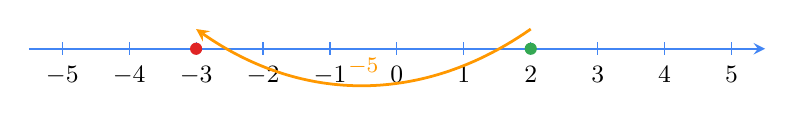
\begin{tikzpicture}[x=0.85cm,>=stealth]
\draw[->,thick,Navy] (-5.5,0)--(5.5,0);
\foreach \i in {-5,...,5}{\draw[Navy] (\i,0.08)--(\i,-0.08); \node[below,font=\small] at (\i,-0.1){$\i$};}
\draw[->,tmOrange,line width=1pt] (2,0.25) to[bend left=35] node[above,font=\footnotesize]{$-5$} (-3,0.25);
\fill[tmGreen] (2,0) circle (2.2pt); \fill[AnsRed] (-3,0) circle (2.2pt);
\end{tikzpicture}\end{center}
\emph{Example:} $2+(-5)=-3$: starting at $2$, move $5$ steps to the left and arrive at $-3$.

\textbf{2. Adding and subtracting integers.}
\begin{itemize}[leftmargin=1.4em,itemsep=1pt,topsep=2pt]
\item Two numbers with the same sign: add the sizes and keep the common sign: $(-11)+(-26)=-37$.
\item Two numbers with different signs: subtract the smaller size from the larger one and take the sign of the number with the larger size: $11+(-37)=-26$.
\item Subtracting means adding the opposite: $a-b=a+(-b)$. Example: $-26-11=-26+(-11)=-37$.
\end{itemize}

\textbf{3. Order of operations.} Brackets first $\to$ powers $\to$ multiplication and division (left to right)
$\to$ addition and subtraction (left to right). Example: $6+2\cdot 3=6+6=12$ (not $8\cdot 3$).

\textbf{4. The distributive law.} $a(b+c)=ab+ac$ and $a(b-c)=ab-ac$.
\emph{Examples:} $3(T+4)=3T+12$;\quad $20\cdot 9\,000-20\cdot 6\,750=20\cdot(9\,000-6\,750)$.

\textbf{5. Simplifying expressions.} Add ``like terms'': $3x+5x=8x$; \
$(a+1)+(b+1)+(c+1)+(d+1)=(a+b+c+d)+4$.

\textbf{6. Points in the coordinate plane.} The point $(x,y)$ has $x$-coordinate $x$ and $y$-coordinate $y$. Moving $k$ units
to the right increases $x$ by $k$; moving $k$ units up increases $y$ by $k$ (moving left or down decreases them).
\end{knowbox}

\begin{proofbox}
\textbf{Why is $a(b+c)=ab+ac$?} Take a rectangle with width $a$ and length $b+c$. Its area is
$a(b+c)$. But we can also cut it into two smaller rectangles with areas $ab$ and $ac$. It is the same
area, so $a(b+c)=ab+ac$.
\begin{figC}
\fill[tmBlue!18] (0,0) rectangle (3,1.2); \fill[tmGreen!20] (3,0) rectangle (5,1.2);
\draw[Navy,line width=0.9pt] (0,0) rectangle (5,1.2); \draw[Navy,line width=0.9pt] (3,0)--(3,1.2);
\node at (1.5,0.6){$ab$}; \node at (4,0.6){$ac$};
\node[left] at (0,0.6){$a$}; \node[below] at (1.5,0){$b$}; \node[below] at (4,0){$c$};
\end{figC}
\end{proofbox}

\begin{warnbox}
$3(T+4)$ is \emph{not} equal to $3T+4$: you must multiply $3$ by \emph{each} term inside the brackets, $3(T+4)=3T+3\cdot 4=3T+12$.
Likewise $-(a-b)=-a+b$ (change the sign of \emph{every} term in the brackets).
\end{warnbox}

% ------------------------------------------------------------------------------------------
\needspace{6\baselineskip}\shead{Equations and the balance principle}
\begin{knowbox}
\textbf{1. Equations.} A statement of equality containing an unknown, such as $2(x+8)=38$, is called an \textbf{equation}.
A number that makes both sides equal when it replaces the unknown is called a \textbf{solution}. To \emph{solve an equation} means to find its solutions.

\textbf{2. The balance principle.} Imagine the equation as a pair of scales in balance.
The scales stay balanced if we:
\begin{itemize}[leftmargin=1.4em,itemsep=1pt,topsep=2pt]
\item add (or subtract) \emph{the same number} on both sides;
\item multiply (or divide) both sides by \emph{the same non-zero number}.
\end{itemize}
A familiar consequence is the \textbf{rule for moving terms}: when a term moves from one side to the other, its \emph{sign changes}.

\begin{center}
\aeaScale{\aeaSq\,\aeaSq\ \ \fbox{\footnotesize 3 kg}}{\fbox{\footnotesize 11 kg}}
\end{center}
\emph{Example:} two identical boxes plus a $3$ kg weight balance $11$ kg: $2x+3=11$.
Remove the $3$ kg weight from both pans: $2x=11-3=8$. Halve both pans: $x=8\div 2=4$. Each box weighs $4$ kg.

\textbf{3. Substitution on scales.} If $A$ on one pan balances $B$, then on any other pair of scales we may
replace $A$ by $B$ and the scales stay balanced (just like replacing an expression by an equal expression).

\textbf{4. Always check.} After solving, substitute the solution into the original equation to make sure both sides are equal.
\end{knowbox}

\begin{proofbox}
\textbf{Why does a term change sign when it moves across?} From $2x+3=11$, subtract $3$ from both sides (the scales stay balanced):
$2x+3-3=11-3$, that is, $2x=11-3$. Looking at the result, the term $+3$ on the left seems to have ``jumped'' to the right and become $-3$.
In fact nothing ``jumps'': we only subtracted the same number from both sides.
\end{proofbox}

\begin{warnbox}
Forgetting to change the sign: from $x+11=-26$, writing $x=-26+11$ is \textbf{wrong}. The correct step is $x=-26-11=-37$.
\end{warnbox}

\begin{tipbox}
In a multiple-choice question with an equation, you can \emph{substitute each option in turn} into the equation. It is slower
but very safe, and it is also the best way to check.
\end{tipbox}

% ------------------------------------------------------------------------------------------
\needspace{6\baselineskip}\shead{Solving word problems with equations}
\begin{knowbox}
\textbf{Four steps for a word problem.}
\begin{enumerate}[leftmargin=1.6em,itemsep=1pt,topsep=2pt]
\item \textbf{Choose an unknown}: call the quantity you want (or a related one) $x$; write its unit and any condition (for example $x>0$, $x$ is a whole number).
\item \textbf{Express} the other quantities in terms of $x$.
\item \textbf{Write an equation} from the conditions of the problem and \textbf{solve} it.
\item \textbf{Compare} with the conditions, \textbf{check}, and \textbf{answer} the actual question.
\end{enumerate}

\textbf{Common types.}
\begin{itemize}[leftmargin=1.4em,itemsep=2pt,topsep=2pt]
\item \textbf{Consecutive integers:} $n,\ n+1,\ n+2$ (or, more neatly, $n-1,\ n,\ n+1$). Consecutive even (odd) numbers differ by $2$: $n,\ n+2,\ n+4$.
\item \textbf{Sums in pairs:} three objects $a,b,c$ weighed two at a time give $a+b$, $b+c$, $c+a$. Adding the three results:
$(a+b)+(b+c)+(c+a)=2(a+b+c)$, so \emph{the total of the three objects is half of the sum of the results}. To find one object, subtract the pair formed by the other two from the total.
\item \textbf{Angles in a triangle:} the three angles of a triangle add up to $180^\circ$; an isosceles triangle has two equal base angles.
\item \textbf{Average:} average $=$ sum of the values $\div$ number of values; average price $=$ total cost $\div$ total mass.
\end{itemize}
\end{knowbox}

\textbf{Two small examples.}

\emph{a) An isosceles triangle with a $70^\circ$ angle.} The $70^\circ$ angle may be a \emph{base angle} or the \emph{apex angle}, so we must look at two cases:
\begin{itemize}[leftmargin=1.4em,itemsep=1pt,topsep=1pt]
\item If $70^\circ$ is a base angle: the base angles are $70^\circ$ and $70^\circ$, and the apex angle is $180^\circ-70^\circ-70^\circ=40^\circ$.
\item If $70^\circ$ is the apex angle: the two base angles are equal and add up to $180^\circ-70^\circ=110^\circ$, so each is $55^\circ$.
\end{itemize}
\begin{figC}
\draw[tmBlue,line width=1pt,fill=tmBlue!8] (0,0)--(2.4,0)--(1.2,3.3)--cycle;
\node[font=\footnotesize] at (0.45,0.25){$70^\circ$}; \node[font=\footnotesize] at (1.95,0.25){$70^\circ$}; \node[font=\footnotesize] at (1.2,2.6){$40^\circ$};
\draw[tmOrange!85!black,line width=1pt,fill=tmOrange!10] (4,0)--(7.4,0)--(5.7,2.43)--cycle;
\node[font=\footnotesize] at (4.55,0.22){$55^\circ$}; \node[font=\footnotesize] at (6.85,0.22){$55^\circ$}; \node[font=\footnotesize] at (5.7,1.85){$70^\circ$};
\end{figC}

\emph{b) Average price.} You buy $300$ g of type I candy for $15\,000$ dong and $200$ g of type II candy for $20\,000$ dong. The average price
of $100$ g of candy is $(15\,000+20\,000)\div(300+200)\cdot 100=35\,000\div 500\cdot 100=7\,000$ dong.
You must \emph{not} average the two prices $5\,000$ and $10\,000$ dong per $100$ g (that gives $7\,500$ dong, which is wrong), because different amounts of the two candies were bought.

\begin{proofbox}
\textbf{Three consecutive integers: the middle one equals the sum divided by $3$.} Call the three numbers $n-1$, $n$, $n+1$. Their sum is
$(n-1)+n+(n+1)=3n$ (the $-1$ and $+1$ cancel). So the middle number is $n=\text{sum}\div 3$. For example, if the sum is $153$, the middle number is $51$ and the three numbers are $50,51,52$.
\end{proofbox}

\begin{tipbox}
Choosing the \emph{middle number} as the unknown usually gives the neatest equation. For ``sums in pairs'' problems, do not rush to use three unknowns:
\emph{add everything up} first.
\end{tipbox}

\begin{warnbox}
Solving the equation is not the end of the problem! Re-read the question: does it ask for the \emph{largest} number, the \emph{lightest} object, or the \emph{total}...?
Many students find the correct $x$ but choose the wrong option because they answer a different question.
\end{warnbox}

\begin{parentbox}
When your child is stuck, ask: ``What don't we know yet? Let's call it $x$. Now, what does the problem tell us about $x$?''
Let your child say it in words first, and only then write it as an equation.
\end{parentbox}

% ------------------------------------------------------------------------------------------
\needspace{6\baselineskip}\shead{Patterns, tables of values and arithmetic sequences}
\begin{knowbox}
\textbf{1. Arithmetic sequences.} A list of numbers in which neighbouring numbers always differ by the same number $d$ (called the
\textbf{common difference}) is called an arithmetic sequence. If the first term is $a$, then
\[\text{the } n\text{-th term} \;=\; a+(n-1)\cdot d .\]
\emph{Example:} the sequence $7,10,13,16,\dots$ has $a=7$, $d=3$; its $n$-th term is $7+3(n-1)=3n+4$.

\textbf{2. From a table of values to an expression.} If each time $n$ increases by $1$ the value increases by $d$, the expression has the form
$d\cdot n+\text{(some number)}$. Find ``some number'' by substituting $n=1$.
\begin{center}
\begin{tabular}{|c|c|c|c|c|c|}
\hline
\rowcolor{tmBlue!10} $n$ & $1$ & $2$ & $3$ & $4$ & $5$\\ \hline
value & $4$ & $7$ & $10$ & $13$ & $16$\\ \hline
\end{tabular}
\end{center}
Each time $n$ increases by $1$, the value increases by $3$, so the expression has the form $3n+b$. Substituting $n=1$: $3+b=4$, so $b=1$. Hence value $=3n+1$.

\textbf{3. Is a number in the sequence?} The number $N$ belongs to the sequence $a,\ a+d,\ a+2d,\dots$ exactly when
$N-a$ is divisible by $d$ (and $N\ge a$). For a sequence counting down, $a,\ a-d,\ a-2d,\dots$, look at $a-N$ instead.

\textbf{4. Common terms of two sequences; repeating events.} If two arithmetic sequences with differences $d_1$ and $d_2$ have a common term, then
their common terms are exactly $\text{lcm}(d_1,d_2)$ apart. Similarly, events that repeat every $p$ minutes and every $q$ minutes
happen together again every $\text{lcm}(p,q)$ minutes.
\end{knowbox}

\begin{tipbox}
\emph{An example of repetition.} The first bus returns to the station every $12$ minutes, the second bus every $20$ minutes. At 7:00 a.m. both are at the station.
The first bus returns after $12, 24, 36, 48, \mathbf{60},\dots$ minutes; the second after $20, 40, \mathbf{60},\dots$ minutes.
The two buses meet at the station again every $\text{lcm}(12,20)=60$ minutes, that is, at 8:00 a.m., 9:00 a.m., \dots

Similarly, if the two sequences $7,10,13,\dots$ (difference $3$) and $2011,2006,2001,\dots$ (difference $5$) have a common term, then their common terms are $\text{lcm}(3,5)=15$ apart.
\end{tipbox}

\begin{proofbox}
\textbf{Why is the $n$-th term $a+(n-1)d$?} Going from the $1$st term to the $n$-th term, we cross $n-1$ ``gaps'',
and each gap adds $d$. It is like walking from the $1$st lamp post to the $5$th: you only pass $4$ gaps.
\begin{figC}
\foreach \i/\v in {0/a,1/a+d,2/a+2d,3/a+3d}{\fill[tmBlue] (2.2*\i,0) circle (2.5pt); \node[below,font=\footnotesize] at (2.2*\i,-0.1){$\v$};}
\foreach \i in {0,1,2}{\draw[->,tmOrange,line width=0.9pt] (2.2*\i+0.15,0.15) to[bend left=30] node[above,font=\footnotesize]{$+d$} (2.2*\i+2.05,0.15);}
\node[font=\footnotesize,text=Slate] at (0,0.7){1st}; \node[font=\footnotesize,text=Slate] at (6.6,0.7){4th};
\end{figC}
From the $1$st term to the $4$th term there are $3$ steps of $+d$, so the $4$th term is $a+3d$.
\end{proofbox}

\begin{warnbox}
Checking a formula against only \emph{one} column of the table is not enough. For example, for the table $1,3,5,7,9$, both $3n-2$ and $2n-1$
give the value $1$ when $n=1$, but for $n=2$ we get $3n-2=4\neq 3$. Test \emph{at least two or three columns}.
\end{warnbox}

% ------------------------------------------------------------------------------------------
\needspace{6\baselineskip}\shead{Ratios, units of measurement and uniform motion}
\begin{knowbox}
\textbf{1. Directly proportional quantities.} If one scoop of food feeds $8$ fish, then $2$ scoops feed $16$ fish and $4$ scoops feed $32$ fish:
when the number of scoops is multiplied by some number, the number of fish is multiplied by the same number. We say $y$ is \textbf{directly proportional} to $x$ with constant $k$ if $y=k\cdot x$.
The usual method is the \textbf{unit method} (work out the value for $1$ part first, then multiply).

\textbf{2. Uniform motion.} With $s$ the distance, $v$ the speed and $t$ the time:
\[ s=v\cdot t,\qquad t=\frac{s}{v},\qquad v=\frac{s}{t}.\]
Use matching units: if $v$ is in km/h, then $s$ is in km and $t$ is in hours.

Two people moving \emph{for the same length of time}: whoever is $k$ times as fast covers $k$ times the distance.

\emph{Running in opposite directions around a circle:} from one meeting to the next, the \emph{total} distance run by the two people is exactly one lap.
If the first person is $k$ times as fast as the second, then during each such stretch the first runs $\dfrac{k}{k+1}$ of a lap and the second runs $\dfrac{1}{k+1}$ of a lap.

\textbf{3. Converting units of time.}
$1$ minute $=60$ seconds;\ \ $1$ hour $=60$ minutes $=60\times 60=3\,600$ seconds;\ \ $1$ day $=24$ hours;\ \ $1$ week $=7$ days.
Therefore $1$ week $=7\times 24$ hours $=7\times 24\times 60$ minutes $=7\times 24\times 60\times 60$ seconds.

\textbf{4. Money.} Number of notes $=$ total amount $\div$ value of one note. \ Difference after $n$ times
$=n\times(\text{higher price}-\text{lower price})$.
\end{knowbox}

\begin{tipbox}
Read a product such as $60\times 60\times 24\times 7$ as a \emph{chain of unit conversions}, from right to left:
$7$ (days in a week) $\times 24$ (hours in a day) $\times 60$ (minutes in an hour) $\times 60$ (seconds in a minute).
The result is the number of seconds in one week.
\end{tipbox}

\begin{proofbox}
\textbf{Why can we work out the difference ``per time'' and then multiply?} By the distributive law:
$20\times 9\,000-20\times 6\,750=20\times(9\,000-6\,750)=20\times 2\,250$. Both ways always give the same result,
but the second is much quicker to do in your head.
\end{proofbox}

\begin{warnbox}
In motion problems, read carefully ``how much has been travelled'' and ``how much is left''. After half of a $510$ km trip,
the distance left is $510\div 2=255$ km, not $510$ km.
\end{warnbox}

% ------------------------------------------------------------------------------------------
\needspace{6\baselineskip}\shead{Equivalent fractions and a fraction of a quantity}
\begin{knowbox}
\textbf{1. The basic property.} Multiplying (or dividing) the numerator and the denominator of a fraction by the same non-zero number
gives an equal fraction: $\dfrac{3}{7}=\dfrac{3\cdot 9}{7\cdot 9}=\dfrac{27}{63}$.

\textbf{2. Recognising equal fractions.} For $b\neq 0$, $d\neq 0$:\quad
$\dfrac{a}{b}=\dfrac{c}{d}$ exactly when $a\cdot d=b\cdot c$ (``cross-multiplying'').

\textbf{3. Fractions with the same numerator.} If $\dfrac{1}{p}=\dfrac{1}{q}$ (or $\dfrac{m}{p}=\dfrac{m}{q}$ with $m\neq 0$), then $p=q$.
Two equal fractions with equal numerators also have equal denominators.

\textbf{4. A fraction of a quantity.} To find $\dfrac{m}{n}$ of a number $A$, calculate $A\cdot\dfrac{m}{n}=A\div n\cdot m$.
\emph{Example:} $\dfrac{3}{7}$ of $168$ km is $168\div 7\cdot 3=24\cdot 3=72$ km. The rest corresponds to $1-\dfrac{3}{7}=\dfrac{4}{7}$.
\end{knowbox}

\begin{proofbox}
\textbf{Why does $\dfrac{1}{p}=\dfrac{1}{q}$ imply $p=q$?} Cross-multiply: $1\cdot q=p\cdot 1$, that is, $q=p$.
In other words: if a cake is cut into $p$ pieces and another identical cake into $q$ pieces, and the pieces are the same size, then the numbers of pieces must be the same.
\end{proofbox}

% ------------------------------------------------------------------------------------------
\needspace{6\baselineskip}\shead{Comparing and reasoning about order}
\begin{knowbox}
\textbf{1. The transitive property.} If $a<b$ and $b<c$, then $a<c$. This lets us line up several numbers: $a<b<c<d$.

\textbf{2. The ``set it equal to $k$'' technique.} When several expressions are equal, for example $a-2=b+2=c+1=d-3$, call the common value $k$:
\[a=k+2,\qquad b=k-2,\qquad c=k-1,\qquad d=k+3.\]
Now every number is compared with the same reference point $k$; ordering the ``extras'' $-2<-1<+2<+3$ we get $b<c<a<d$.
\begin{center}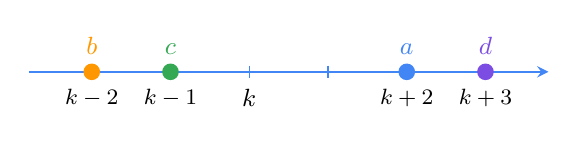
\begin{tikzpicture}[x=1cm,>=stealth]
\draw[->,thick,Navy] (-2.8,0)--(3.8,0);
\foreach \i in {-2,...,3}{\draw[Navy] (\i,0.08)--(\i,-0.08);}
\node[below,font=\small] at (0,-0.1){$k$};
\foreach \i/\l/\c in {-2/b/tmOrange,-1/c/tmGreen,2/a/tmBlue,3/d/tmPurple}{\fill[\c] (\i,0) circle (3pt); \node[above,font=\small\bfseries,text=\c] at (\i,0.1){$\l$};}
\node[below,font=\footnotesize] at (-2,-0.1){$k-2$}; \node[below,font=\footnotesize] at (-1,-0.1){$k-1$};
\node[below,font=\footnotesize] at (2,-0.1){$k+2$}; \node[below,font=\footnotesize] at (3,-0.1){$k+3$};
\end{tikzpicture}\end{center}

\textbf{3. Logical reasoning about order.} For sentences like ``An owns more cats than Bình'', translate them into symbols ($A>B$),
write down all the conditions and link them with the transitive property. A statement that ``\emph{must be true}'' has to be true in
\emph{every} situation that fits the problem; a single counter-example is enough to reject it.
\end{knowbox}

\begin{tipbox}
\emph{A reasoning example.} An is taller than Bình; Chi is shorter than Bình; Dũng is taller than Chi. Who is the shortest?
In symbols: $A>B$, \ $B>C$, \ $D>C$. From $A>B>C$ and $D>C$ we see that $A$, $B$ and $D$ are all taller than $C$: \textbf{Chi is the shortest}.
But we do \emph{not} know whether Dũng is taller or shorter than An (for instance, if An is $1.6$ m, Bình $1.5$ m and Chi $1.2$ m, then Dũng being $1.7$ m or $1.3$ m both fit all the conditions), so the statement ``Dũng is the tallest'' is \emph{not necessarily} true.
\end{tipbox}

\begin{warnbox}
Seeing that $a-2$ and $b+2$ are equal, many students conclude too quickly that ``$a$ is smaller because something is subtracted''. The opposite is true:
$a$ must \emph{lose} $2$ to equal $b$ \emph{plus} $2$, so $a$ is exactly $4$ more than $b$.
\end{warnbox}

\begin{parentbox}
Use real objects: ``If your bag loses $2$ marbles, it has the same number as my bag plus $2$ marbles. Which bag has more?''
Let your child check with marbles. A concrete picture keeps the child from being fooled by plus and minus signs.
\end{parentbox}

% ==========================================================================================
\needspace{6\baselineskip}\shead{Worked examples}

\begin{exbox}{Example 1 \ (Translating words and evaluating an expression)}
\textbf{a)} Evaluate the expression $A=2x^2-3x+1$ for $x=-2$.

\textbf{b)} Hoa has $50\,000$ dong in her piggy bank. Every week she puts in another $20\,000$ dong.
Write an expression for the amount in the piggy bank after $t$ weeks, then work out that amount after $6$ weeks.
\guide
\step{1}{Part a: substitute $x=-2$, remembering the brackets}
\[A=2\cdot(-2)^2-3\cdot(-2)+1.\]
\step{2}{Calculate in order: powers $\to$ multiplication $\to$ addition and subtraction}
$(-2)^2=(-2)\cdot(-2)=4$, so $2\cdot 4=8$. \ $3\cdot(-2)=-6$, so $-3\cdot(-2)=+6$. Hence $A=8+6+1=15$.
\step{3}{Part b: find the pattern with a small table}
\begin{center}
\begin{tabular}{|c|c|c|c|c|}
\hline
\rowcolor{tmBlue!10} Weeks & $0$ & $1$ & $2$ & $t$\\ \hline
Amount (dong) & $50\,000$ & $50\,000+20\,000$ & $50\,000+2\cdot 20\,000$ & $50\,000+20\,000t$\\ \hline
\end{tabular}
\end{center}
The starting amount stays the same; the added part is $20\,000$ times the number of weeks. Expression: $50\,000+20\,000t$ (dong).
\step{4}{Substitute $t=6$}
$50\,000+20\,000\cdot 6=50\,000+120\,000=170\,000$ (dong).
\begin{warnbox}Do not write $(50\,000+20\,000)\cdot t$: the starting amount is there only \emph{once}; it must not be multiplied by the number of weeks.\end{warnbox}
\ans{a) $A=15$;\ \ b) $50\,000+20\,000t$ dong; after $6$ weeks there are $170\,000$ dong.}
\end{exbox}

\begin{exbox}{Example 2 \ (Solving equations with the balance principle)}
Solve the equations:\quad \textbf{a)} $5x-7=2x+11$;\qquad \textbf{b)} $\dfrac{x}{12}=\dfrac{5}{4}$.
\guide
\step{1}{Part a: collect the terms with $x$ on the left}
Subtract $2x$ from both sides: $5x-2x-7=11$, that is, $3x-7=11$.
\step{2}{Collect the numbers on the right}
Add $7$ to both sides: $3x=11+7=18$.
\step{3}{Divide both sides by $3$}
$x=18\div 3=6$.
\verify{Left side: $5\cdot 6-7=30-7=23$. Right side: $2\cdot 6+11=12+11=23$. Both sides are equal.}
\step{4}{Part b: use a common denominator (or cross-multiply)}
We have $\dfrac{5}{4}=\dfrac{5\cdot 3}{4\cdot 3}=\dfrac{15}{12}$. The fractions $\dfrac{x}{12}$ and $\dfrac{15}{12}$ have the same denominator
and are equal, so $x=15$. (Cross-multiplying also works: $4x=12\cdot 5=60$, $x=60\div 4=15$.)
\begin{recallbox}$\dfrac{a}{b}=\dfrac{c}{d}$ exactly when $ad=bc$ ($b,d\neq 0$).\end{recallbox}
\ans{a) $x=6$;\ \ b) $x=15$.}
\end{exbox}

\begin{exbox}{Example 3 \ (Consecutive even numbers)}
The sum of four consecutive even numbers is $116$. Find the largest of the four numbers.
\guide
\step{1}{Choose an unknown}
Let the smallest even number be $n$ ($n$ is even). Consecutive even numbers differ by $2$, so the four numbers are
$n,\ n+2,\ n+4,\ n+6$.
\step{2}{Write an equation}
$n+(n+2)+(n+4)+(n+6)=116$, that is, $4n+12=116$.
\step{3}{Solve}
$4n=116-12=104$, \ $n=104\div 4=26$. The four numbers are $26,\ 28,\ 30,\ 32$.
\verify{$26+28+30+32=116$. Correct.}
\step{4}{Answer the actual question}
The question asks for the \emph{largest} number: it is $32$.
\begin{tipbox}Mental shortcut: the four numbers are equally spaced, so their average $116\div 4=29$ lies exactly halfway between the two middle numbers $28$ and $30$. The four numbers follow at once.\end{tipbox}
\ans{$32$}
\end{exbox}

\begin{exbox}{Example 4 \ (Weighing in pairs)}
Three friends, Mai, Lan and Hoa, step on a scale two at a time. Mai and Lan weigh $72$ kg; Mai and Hoa weigh $78$ kg;
Lan and Hoa weigh $80$ kg. How many kilograms does each girl weigh?
\guide
\step{1}{Add all three weighings}
In the three weighings, each girl is weighed exactly \emph{twice}:
$(M+L)+(M+H)+(L+H)=72+78+80=230$, that is, $2(M+L+H)=230$.
\step{2}{Total mass of the three girls}
$M+L+H=230\div 2=115$ (kg).
\step{3}{Find each girl: subtract the pair that does not contain her from the total}
Hoa $=115-(M+L)=115-72=43$ kg;\quad Lan $=115-(M+H)=115-78=37$ kg;\quad Mai $=115-(L+H)=115-80=35$ kg.
\begin{figC}
\foreach \y/\a/\b/\ca/\cb/\s in {0/Mai/Lan/tmBlue/tmOrange/72,-0.8/Mai/Hoa/tmBlue/tmGreen/78,-1.6/Lan/Hoa/tmOrange/tmGreen/80}{
  \node[draw=\ca!80!black,fill=\ca!15,rounded corners=2pt,minimum width=1.4cm] at (0,\y){\a};
  \node at (0.95,\y){$+$};
  \node[draw=\cb!80!black,fill=\cb!15,rounded corners=2pt,minimum width=1.4cm] at (1.9,\y){\b};
  \node[anchor=west] at (2.7,\y){$=\s$ kg};}
\end{figC}
\verify{$35+37=72$, \ $35+43=78$, \ $37+43=80$. All three weighings match.}
\ans{Mai $35$ kg, Lan $37$ kg, Hoa $43$ kg.}
\end{exbox}

\begin{exbox}{Example 5 \ (Arithmetic sequences)}
Consider the sequence $4,\ 7,\ 10,\ 13,\ \dots$ (each number is $3$ more than the one before).
\textbf{a)} Write an expression for the $n$-th term.\quad \textbf{b)} Find the $50$th term.\quad
\textbf{c)} Is $2026$ in the sequence? If so, which term is it?
\guide
\step{1}{The $n$-th term}
First term $a=4$, common difference $d=3$: the $n$-th term is $4+3(n-1)=4+3n-3=3n+1$.
\begin{recallbox}The $n$-th term of an arithmetic sequence $=a+(n-1)d$.\end{recallbox}
\step{2}{The $50$th term}
$3\cdot 50+1=151$.
\step{3}{Test the number $2026$}
We need a whole number $n$ with $3n+1=2026$, that is, $3n=2025$. Since $2025\div 3=675$ exactly, $n=675$.
\verify{$3\cdot 675+1=2025+1=2026$. Correct.}
\begin{warnbox}Do not forget to check that the division is exact. For instance, $2027$ is \emph{not} in the sequence because $2026$ is not divisible by $3$.\end{warnbox}
\ans{a) $3n+1$;\ \ b) $151$;\ \ c) yes, it is the $675$th term.}
\end{exbox}

\begin{exbox}{Example 6 \ (Motion, fractions and unit conversion)}
A train travels at a constant speed of $72$ km/h on a $360$ km route. It has already covered $\dfrac{2}{3}$ of the route.
How much longer (in hours and minutes) does the train need to reach its destination?
\guide
\step{1}{Distance already covered}
$\dfrac{2}{3}$ of $360$ km is $360\div 3\cdot 2=120\cdot 2=240$ km.
\step{2}{Distance left}
$360-240=120$ km. (Or: the remaining part is $1-\dfrac{2}{3}=\dfrac{1}{3}$ of the route, $360\div 3=120$ km.)
\begin{barfigC}
\blk{0}{5}{0}{0.55}{tmBlue}{covered 240 km}
\blk{5}{7.5}{0}{0.55}{tmOrange}{left 120 km}
\brcup{0}{7.5}{0.55}{360 km}
\end{barfigC}
\step{3}{Time left}
\begin{recallbox}$t=\dfrac{s}{v}$ (time $=$ distance $\div$ speed).\end{recallbox}
$t=120\div 72=\dfrac{120}{72}=\dfrac{5}{3}$ hours $=1\dfrac{2}{3}$ hours.
\step{4}{Convert to hours and minutes}
$\dfrac{2}{3}$ hour $=\dfrac{2}{3}\cdot 60=40$ minutes. So $t=1$ hour $40$ minutes.
\verify{In $1$ hour $40$ minutes $=\dfrac{5}{3}$ hours, the train covers $72\cdot\dfrac{5}{3}=24\cdot 5=120$ km, exactly the distance left.}
\ans{$1$ hour $40$ minutes.}
\end{exbox}

\begin{exbox}{Example 7 \ (A balance-scale problem)}
Both scales below are balanced. Identical shapes have equal weights.
\begin{center}
\aeaScale{\aeaSq}{\aeaTri\,\aeaCir}\hspace{1.2cm}\aeaScale{\aeaSq\,\aeaCir}{\aeaTri\,\aeaTri\,\aeaTri}
\end{center}
How many circles \aeaCir\ balance two squares \aeaSq\,\aeaSq?
\guide
\step{1}{Write each scale as an equation}
Let $S$, $T$, $C$ be the weights of a square, a triangle and a circle. Scale 1: $S=T+C$. \ Scale 2: $S+C=3T$.
\step{2}{Substitute scale 1 into scale 2}
On scale 2, replace the square by ``one triangle and one circle'' (allowed by scale 1):
$T+C+C=3T$.
\step{3}{Remove identical things from both pans}
Remove one triangle from each pan: $C+C=T+T$, that is, $2C=2T$, so $C=T$: a circle weighs the same as a triangle.
\step{4}{Answer}
$S=T+C=C+C=2C$, so $2S=4C$: two squares balance $4$ circles.
\verify{Try $C=T=1$, $S=2$: scale 1: $2=1+1$; scale 2: $2+1=3$. Both are correct.}
\ans{$4$ circles.}
\end{exbox}

\begin{exbox}{Example 8 \ (Ordering with the ``set it equal to $k$'' technique)}
The positive integers $a$, $b$, $c$ (all greater than $5$) satisfy\quad
$\dfrac{2}{a+3}=\dfrac{2}{b-1}=\dfrac{2}{c+5}$. Arrange $a$, $b$, $c$ in increasing order.
\guide
\step{1}{Equal fractions with the same numerator have equal denominators}
The three fractions all have numerator $2$ and are equal, so their denominators are equal: $a+3=b-1=c+5$.
\begin{recallbox}If $\dfrac{m}{p}=\dfrac{m}{q}$ with $m\neq 0$, then $p=q$.\end{recallbox}
\step{2}{Call the common value $k$}
$a+3=k\Rightarrow a=k-3$;\quad $b-1=k\Rightarrow b=k+1$;\quad $c+5=k\Rightarrow c=k-5$.
\step{3}{Compare with the reference point $k$}
$k-5<k-3<k+1$, so $c<a<b$.
\verify{Take $k=12$: $a=9$, $b=13$, $c=7$. Then $\dfrac{2}{12}=\dfrac{2}{12}=\dfrac{2}{12}$ and indeed $7<9<13$.}
\ans{$c<a<b$.}
\end{exbox}

% ==========================================================================================
\clearpage
\dividerbar{Core practice}

% ---------------------------------------------------------------- Problem 1
\begin{probbox}{1}{\relax}
Mr Tâm drives a car at a constant speed of $85$ km/h on a $510$ km trip. He has now covered exactly
half of the distance. How many more hours does he need to finish the trip?
\choices{$5$ hours}{$425$ hours}{$12$ hours}{$1.5$ hours}{$3$ hours}
\end{probbox}
\probsol{
\textbf{Understanding the problem.} \emph{Given:} speed $85$ km/h (constant), whole trip $510$ km, half already covered.
\emph{Find:} the time needed for the remaining part.
\step{1}{Work out the distance left}
Half has been covered, so exactly half is left: $510\div 2=255$ (km).
\begin{barfigC}
\blk{0}{3}{0}{0.55}{tmBlue}{covered 255 km}
\blk{3}{6}{0}{0.55}{tmOrange}{left 255 km}
\brcup{0}{6}{0.55}{510 km}
\end{barfigC}
\step{2}{Work out the time for the remaining distance}
\begin{recallbox}Distance $=$ speed $\times$ time, so time $=$ distance $\div$ speed ($t=\dfrac{s}{v}$).\end{recallbox}
$t=255\div 85=3$ (hours). (Mentally: $85\times 3=255$.)
\begin{warnbox}Calculating $510\div 85=6$ hours gives the time for the \emph{whole} trip, which does not answer the question. And $510-85=425$ is a meaningless calculation (km minus km/h); that is the trap in option (B).\end{warnbox}
\begin{tipbox}Another way: the whole trip takes $510\div 85=6$ hours; covering half the distance (at a constant speed) means half the time has passed, so $6\div 2=3$ hours are left.\end{tipbox}
\verify{In $3$ hours the car covers $85\times 3=255$ km, exactly the distance left.}
The result $3$ hours is option \textbf{(E)}.
\ans{(E) $3$ hours}
}

% ---------------------------------------------------------------- Problem 2
\begin{probbox}{2}{\relax}
In the diagram, the triangle has one side of length $14$ cm and two equal sides of length $12$ cm each; the rectangle has width
$8$ cm and length $x$ cm. The perimeter of the triangle equals the perimeter of the rectangle. Find $x$.
\begin{figC}
\draw[tmBlue,line width=1.1pt,fill=tmBlue!10] (0,2.6)--(2.8,2.6)--(1.4,1.2)--cycle;
\node[above] at (1.4,2.6){$14$ cm};
\node[right] at (2.15,1.9){$12$ cm};
\draw[tmBlue,line width=0.9pt] ($(0.7,1.9)+(-0.1,-0.1)$)--($(0.7,1.9)+(0.1,0.1)$);
\draw[tmBlue,line width=0.9pt] ($(2.1,1.9)+(-0.1,0.1)$)--($(2.1,1.9)+(0.1,-0.1)$);
\draw[tmOrange!85!black,line width=1.1pt,fill=tmOrange!12] (0.4,0)rectangle(2.4,0.9);
\node[right] at (2.4,0.45){$8$ cm};
\node[below] at (1.4,0){$x$ cm};
\end{figC}
\choices{$8$}{$10$}{$11$}{$14$}{$15$}
\end{probbox}
\probsol{
\textbf{Understanding the problem.} The triangle has sides $14$ cm, $12$ cm, $12$ cm (the small tick marks show that those two sides are equal).
The rectangle measures $x$ cm by $8$ cm. The two perimeters are equal. We must find $x$.
\step{1}{Work out the perimeter of the triangle}
\begin{recallbox}The perimeter of a triangle is the sum of its three sides. The perimeter of a rectangle is $2\times(\text{length}+\text{width})$.\end{recallbox}
Perimeter of the triangle: $14+12+12=38$ (cm).
\begin{warnbox}The number $12$ is written only once in the diagram, but there are \emph{two} sides of $12$ cm (marked as equal). Forgetting the third side gives $26$ cm and a wrong answer.\end{warnbox}
\step{2}{Write an equation}
The perimeter of the rectangle is $2(x+8)$. Setting the two perimeters equal: $2(x+8)=38$.
\step{3}{Solve the equation}
Divide both sides by $2$: $x+8=19$. Subtract $8$ from both sides: $x=19-8=11$.
\verify{An $11$ cm $\times$ $8$ cm rectangle has perimeter $11+8+11+8=38$ cm, the same as the triangle.}
The value $x=11$ is option \textbf{(C)}.
\begin{parentbox}You can illustrate this with a piece of string $38$ cm long: bend it into a $14$ -- $12$ -- $12$ triangle, then reshape it into a rectangle with an $8$ cm side. Your child will see that the ``perimeter'' is just the length of the string, which does not change when the shape changes.\end{parentbox}
\ans{(C) $11$}
}

% ---------------------------------------------------------------- Problem 3
\begin{probbox}{3}{\relax}
Let $x=3$. Which of the following equations is true?
\choices{$2x=5$}{$3x-1=8$}{$x+5=3$}{$7-x=2$}{$6+2x=14$}
\end{probbox}
\probsol{
\textbf{Understanding the problem.} Substitute $x=3$ into the left side of each equation, work it out, and compare with the right side. Only one equation is true.
\begin{recallbox}To evaluate an expression, replace the letter by the number and calculate in order: multiplication and division first, then addition and subtraction.\end{recallbox}
\step{1}{Check each option in turn}
\begin{center}
\begin{tabular}{|c|l|c|c|}
\hline
\rowcolor{tmBlue!10} Option & Left side with $x=3$ & Right side & True/False\\ \hline
(A) & $2x=2\cdot 3=6$ & $5$ & False\\ \hline
(B) & $3x-1=3\cdot 3-1=9-1=8$ & $8$ & \textbf{True}\\ \hline
(C) & $x+5=3+5=8$ & $3$ & False\\ \hline
(D) & $7-x=7-3=4$ & $2$ & False\\ \hline
(E) & $6+2x=6+2\cdot 3=6+6=12$ & $14$ & False\\ \hline
\end{tabular}
\end{center}
\begin{warnbox}In (E), working in the wrong order, $(6+2)\cdot 3=24$, or reading $2x$ as ``$23$'' leads to mistakes. Multiply first, then add: $6+2\cdot 3=12$.\end{warnbox}
\step{2}{Conclusion}
Only the equation in (B) is true: $3\cdot 3-1=8$. So the answer is \textbf{(B)}.
\ans{(B) $3x-1=8$}
}

% ---------------------------------------------------------------- Problem 4
\begin{probbox}{4}{\relax}
The sum of three consecutive integers is $153$. The largest of the three integers is
\choices{$52$}{$50$}{$53$}{$54$}{$51$}
\end{probbox}
\probsol{
\textbf{Understanding the problem.} Three consecutive integers stand next to each other on the number line and differ by $1$ (for example $7,8,9$). Their sum is $153$. We want the \emph{largest} one.
\step{1}{Choose an unknown: let the middle number be $n$}
The three numbers are $n-1$, \ $n$, \ $n+1$.
\step{2}{Write an equation}
$(n-1)+n+(n+1)=153$. On the left, $-1$ and $+1$ cancel, leaving $3n=153$.
\step{3}{Solve}
$n=153\div 3=51$. The three numbers are $50$, $51$, $52$.
\begin{recallbox}For three consecutive integers, the middle number equals the sum divided by $3$ (the middle number is the average).\end{recallbox}
\begin{proofbox}Another way, letting the smallest number be $m$: $m+(m+1)+(m+2)=3m+3=153$, so $3m=150$, $m=50$. The same three numbers $50,51,52$.\end{proofbox}
\begin{tipbox}Multiple-choice shortcut: the largest number must be a little more than the average $153\div 3=51$; try $50+51+52=153$ straight away.\end{tipbox}
\verify{$50+51+52=153$. Correct.}
\step{4}{Answer the actual question}
The largest number is $52$, which is option \textbf{(A)}.
\begin{warnbox}Option (E) $51$ is the \emph{middle} number and option (B) $50$ is the \emph{smallest} number. Read the question carefully so you do not choose the wrong one.\end{warnbox}
\ans{(A) $52$}
}

% ---------------------------------------------------------------- Problem 5
\begin{probbox}{5}{\relax}
One scoop of fish food can feed $8$ goldfish. How many goldfish can $4$ such scoops of fish food feed?
\choices{$12$}{$16$}{$8$}{$64$}{$32$}
\end{probbox}
\probsol{
\textbf{Understanding the problem.} $1$ scoop $\to$ $8$ fish. Asked: $4$ scoops $\to$ ? fish.
When the number of scoops is multiplied by some number, the number of fish fed is multiplied by the same number (the quantities are directly proportional).
\begin{recallbox}If $y$ is directly proportional to $x$ with constant $k$, then $y=k\cdot x$. Here $k=8$ (fish per scoop), so number of fish $=8\times$ number of scoops.\end{recallbox}
\step{1}{Draw a diagram}
\begin{barfigC}
\blk{0}{1.5}{0}{0.55}{tmGreen}{8 fish}
\blk{1.5}{3}{0}{0.55}{tmGreen}{8 fish}
\blk{3}{4.5}{0}{0.55}{tmGreen}{8 fish}
\blk{4.5}{6}{0}{0.55}{tmGreen}{8 fish}
\brcup{0}{6}{0.55}{4 scoops}
\end{barfigC}
\step{2}{Calculate}
$4\times 8=32$ (fish).
\begin{warnbox}Option (A) $12$ is $8+4$ (adding instead of multiplying), and option (D) $64$ is $8\times 8$. Each extra scoop feeds \emph{$8$ more fish}, so multiply $8$ by the number of scoops.\end{warnbox}
\verify{$32\div 4=8$: exactly $8$ fish per scoop.}
So the answer is \textbf{(E)}.
\ans{(E) $32$}
}

% ---------------------------------------------------------------- Problem 6
\begin{probbox}{6}{\relax}
If $x=4$ and $y=3x$, the value of $y$ is
\choices{$12$}{$24$}{$7$}{$81$}{$4$}
\end{probbox}
\probsol{
\textbf{Understanding the problem.} We know $x=4$. The expression $y=3x$ means ``$y$ equals $3$ times $x$''. We must find $y$.
\begin{recallbox}$3x$ is short for $3\cdot x$ (between a number and a letter we leave out the multiplication sign).\end{recallbox}
\step{1}{Substitute $x=4$}
$y=3\cdot x=3\cdot 4=12$.
\begin{warnbox}Do not read $3x$ as ``$34$'' (joining the digits); it is not $3+4=7$ (option C) or $3^4=81$ (option D) either.\end{warnbox}
\begin{tipbox}Read $y=3x$ in words: ``$y$ is three times $x$''. Three times $4$ is $12$.\end{tipbox}
\verify{$12\div 3=4=x$. Correct.}
So the answer is \textbf{(A)}.
\ans{(A) $12$}
}

% ---------------------------------------------------------------- Problem 7
\begin{probbox}{7}{\relax}
Each bus ride costs Lan $6\,750$ dong, while Minh pays $9\,000$ dong per ride (they use different routes).
If each of them rides the bus $20$ times, how much less does Lan pay than Minh in total?
\choicesII{$75\,000$ dong}{$30\,000$ dong}{$45\,000$ dong}{$135\,000$ dong}{$180\,000$ dong}
\end{probbox}
\probsol{
\textbf{Understanding the problem.} Per ride: Lan $6\,750$ dong, Minh $9\,000$ dong. Each rides $20$ times. We want the \emph{difference} after $20$ rides.
\step{1}{Method 1 -- Work out each total and subtract}
Lan pays: $20\times 6\,750=135\,000$ (dong).\quad Minh pays: $20\times 9\,000=180\,000$ (dong).\\
Difference: $180\,000-135\,000=45\,000$ (dong).
\step{2}{Method 2 -- Work out the difference per ride and multiply (quicker)}
Each ride, Lan pays less than Minh by: $9\,000-6\,750=2\,250$ (dong).\\
After $20$ rides: $20\times 2\,250=45\,000$ (dong).
\begin{recallbox}The distributive law: $20\times 9\,000-20\times 6\,750=20\times(9\,000-6\,750)$. That is why both methods always agree.\end{recallbox}
\begin{warnbox}Option (D) $135\,000$ dong is \emph{Lan's total} and option (E) $180\,000$ dong is \emph{Minh's total}. The question asks how much \emph{less}, which is the difference.\end{warnbox}
\verify{$135\,000+45\,000=180\,000$. Correct.}
So the answer is \textbf{(C)}.
\ans{(C) $45\,000$ dong}
}

% ---------------------------------------------------------------- Problem 8
\begin{probbox}{8}{\relax}
Which expression produces the values in the second row of the table, given the values of $n$ in the first row?
\begin{center}
\begin{tabular}{|c|c|c|c|c|c|}
\hline
\rowcolor{tmBlue!10} $n$ & $1$ & $2$ & $3$ & $4$ & $5$\\ \hline
Value & $1$ & $3$ & $5$ & $7$ & $9$\\ \hline
\end{tabular}
\end{center}
\choices{$3n-2$}{$2(n-1)$}{$n+4$}{$2n$}{$2n-1$}
\end{probbox}
\probsol{
\textbf{Understanding the problem.} We need an expression in $n$ which gives $1,3,5,7,9$ when $n=1,2,3,4,5$.
\step{1}{Find the pattern in the row of values}
Each time $n$ increases by $1$, the value increases by $2$ ($1\to 3\to 5\to 7\to 9$). So the expression has the form $2n+b$.
\begin{recallbox}If the value always increases by $d$ when $n$ increases by $1$, the expression has the form $d\cdot n+b$; find $b$ by substituting $n=1$.\end{recallbox}
\step{2}{Find $b$}
Substitute $n=1$: $2\cdot 1+b=1$, so $b=1-2=-1$. The expression is $2n-1$.
\step{3}{Check the whole table and rule out the other options}
\begin{center}
\begin{tabular}{|c|c|c|c|c|c|c|}
\hline
\rowcolor{tmBlue!10} $n$ & $1$ & $2$ & $3$ & $4$ & $5$ & Verdict\\ \hline
(A) $3n-2$ & $1$ & $4$ & & & & fails at $n=2$\\ \hline
(B) $2(n-1)$ & $0$ & & & & & fails at $n=1$\\ \hline
(C) $n+4$ & $5$ & & & & & fails at $n=1$\\ \hline
(D) $2n$ & $2$ & & & & & fails at $n=1$\\ \hline
(E) $2n-1$ & $1$ & $3$ & $5$ & $7$ & $9$ & \textbf{fits the whole table}\\ \hline
\end{tabular}
\end{center}
\begin{warnbox}Option (A) $3n-2$ also gives $1$ when $n=1$. If you only test the first column, you cannot decide between (A) and (E). Test other columns too.\end{warnbox}
\verify{$2n-1$ for $n=1,2,3,4,5$: $1,3,5,7,9$. It matches the whole table.}
So the answer is \textbf{(E)}.
\ans{(E) $2n-1$}
}

% ---------------------------------------------------------------- Problem 9
\begin{probbox}{9}{\relax}
When two numbers are added, the result is $-26$. One of the numbers is $11$. The other number is
\choices{$-37$}{$37$}{$-15$}{$15$}{$-48$}
\end{probbox}
\probsol{
\textbf{Understanding the problem.} Call the unknown number $x$. We are told that $x+11=-26$. We must find $x$.
\step{1}{Write an equation}
$x+11=-26$.
\step{2}{Solve with the balance principle}
Subtract $11$ from both sides: $x=-26-11$.
\begin{recallbox}Subtracting a number means adding its opposite: $-26-11=-26+(-11)$. Adding two negative numbers: add the sizes and keep the ``$-$'' sign: $-(26+11)=-37$.\end{recallbox}
So $x=-37$.
\begin{center}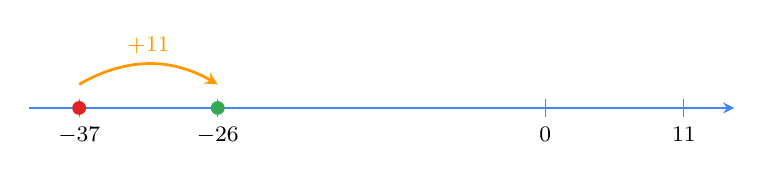
\begin{tikzpicture}[x=0.16cm,>=stealth]
\draw[->,thick,Navy] (-41,0)--(15,0);
\foreach \i in {-37,-26,0,11}{\draw[Navy] (\i,0.12)--(\i,-0.12); \node[below,font=\footnotesize] at (\i,-0.12){$\i$};}
\fill[AnsRed] (-37,0) circle (2.5pt); \fill[tmGreen] (-26,0) circle (2.5pt);
\draw[->,tmOrange,line width=1pt] (-37,0.3) to[bend left=30] node[above,font=\footnotesize]{$+11$} (-26,0.3);
\end{tikzpicture}\end{center}
On the number line: starting from $-37$ and moving $11$ steps to the right, we arrive at $-26$.
\begin{warnbox}Forgetting to change the sign when moving a term across, and writing $x=-26+11=-15$, is wrong (option C). Check: $-15+11=-4\neq -26$.\end{warnbox}
\begin{parentbox}You can explain it with a story about owing money: ``After someone gives you $11$ thousand, you still owe $26$ thousand. How much did you owe at first?'' At first you owed more: $26+11=37$ thousand, that is, $-37$.\end{parentbox}
\verify{$(-37)+11=-26$. Correct.}
So the answer is \textbf{(A)}.
\ans{(A) $-37$}
}

% ---------------------------------------------------------------- Problem 10
\begin{probbox}{10}{\relax}
Mr Hùng has $10\,000\,000$ dong, all in $50\,000$ dong notes. How many notes does he have?
\choices{$1\,000$}{$200$}{$1\,250$}{$500$}{$2\,000$}
\end{probbox}
\probsol{
\textbf{Understanding the problem.} The total amount is $10\,000\,000$ dong (ten million dong). Each note is worth $50\,000$ dong. We must find the number of notes.
\begin{recallbox}Number of notes $=$ total amount $\div$ value of one note.\end{recallbox}
\step{1}{Set up the division}
Number of notes $=10\,000\,000\div 50\,000$.
\step{2}{Simplify by removing zeros}
Remove four zeros from both numbers (that is, divide both by $10\,000$; the quotient does not change): $10\,000\,000\div 50\,000=1\,000\div 5=200$.
\step{3}{Another way of thinking}
$2$ notes of $50\,000$ dong make $100\,000$ dong. Ten million dong is $100$ times $100\,000$ dong, so there are $100\times 2=200$ notes.
\verify{$200\times 50\,000=10\,000\,000$ dong. Correct.}
\begin{warnbox}Miscounting the zeros is a very common mistake. Write numbers with a space between groups of three digits ($10\,000\,000$) to count accurately.\end{warnbox}
So the answer is \textbf{(B)}.
\begin{parentbox}If you have real banknotes at home, let your child count $10$ notes of $50\,000$ dong ($500\,000$ dong), then ask: how many such bundles make $10$ million? ($20$ bundles, that is, $200$ notes.)\end{parentbox}
\ans{(B) $200$}
}

% ---------------------------------------------------------------- Problem 11
\begin{probbox}{11}{\relax}
The product $60\times 60\times 24\times 7$ equals
\choicesL{the number of minutes in seven weeks}{the number of hours in sixty days}{the number of seconds in seven hours}{the number of seconds in one week}{the number of minutes in twenty-four weeks}
\end{probbox}
\probsol{
\textbf{Understanding the problem.} There is no need to multiply the product out. Read each factor as one step of a time-unit conversion.
\begin{recallbox}$1$ week $=7$ days;\ \ $1$ day $=24$ hours;\ \ $1$ hour $=60$ minutes;\ \ $1$ minute $=60$ seconds.\end{recallbox}
\step{1}{Read the product from right to left}
\begin{itemize}[leftmargin=1.4em,itemsep=1pt,topsep=1pt]
\item $7$ is the number of days in \textbf{one week};
\item $24\times 7$ is the number of hours in one week;
\item $60\times 24\times 7$ is the number of minutes in one week;
\item $60\times 60\times 24\times 7$ is the number of \textbf{seconds} in one week.
\end{itemize}
\step{2}{Check the other options by writing their products}
\begin{center}
\begin{tabular}{|c|l|r|}
\hline
\rowcolor{tmBlue!10} Option & Expression & Value\\ \hline
(A) minutes in $7$ weeks & $60\times 24\times 7\times 7$ & $70\,560$\\ \hline
(B) hours in $60$ days & $24\times 60$ & $1\,440$\\ \hline
(C) seconds in $7$ hours & $60\times 60\times 7$ & $25\,200$\\ \hline
(D) seconds in $1$ week & $60\times 60\times 24\times 7$ & $604\,800$\\ \hline
(E) minutes in $24$ weeks & $60\times 24\times 7\times 24$ & $241\,920$\\ \hline
\end{tabular}
\end{center}
Only option (D) has exactly the product $60\times 60\times 24\times 7=604\,800$.
\begin{warnbox}Seeing the numbers $60$, $24$, $7$ in the wording, many students rush to choose (A) or (E). Match \emph{every} conversion step: (A) is missing one factor $60$ and has an extra factor $7$.\end{warnbox}
So the answer is \textbf{(D)}.
\ans{(D) the number of seconds in one week}
}

% ---------------------------------------------------------------- Problem 12
\begin{probbox}{12}{\stars{1}}
Each of $a$, $b$, $c$, $d$ is a positive integer greater than $3$, and
\[\frac{1}{a-2}=\frac{1}{b+2}=\frac{1}{c+1}=\frac{1}{d-3}.\]
Which ordering of these four numbers is correct?
\choicesII{$a<b<c<d$}{$c<b<a<d$}{$b<a<c<d$}{$d<a<c<b$}{$b<c<a<d$}
\end{probbox}
\probsol{
\textbf{Understanding the problem.} Four fractions with the same numerator $1$ are equal. We must compare $a,b,c,d$.
(The condition ``greater than $3$'' makes sure all the denominators are non-zero, so the fractions make sense.)
\step{1}{Equal fractions with the same numerator have equal denominators}
\begin{recallbox}If $\dfrac{1}{p}=\dfrac{1}{q}$, then $p=q$ (cross-multiply: $1\cdot q=1\cdot p$).\end{recallbox}
Therefore: $a-2=b+2=c+1=d-3$.
\step{2}{Call the common value $k$ and write each number in terms of $k$}
$a-2=k\Rightarrow a=k+2$;\quad $b+2=k\Rightarrow b=k-2$;\quad $c+1=k\Rightarrow c=k-1$;\quad $d-3=k\Rightarrow d=k+3$.
\step{3}{Compare with the same reference point $k$}
The ``extras'' are $-2$ (for $b$), $-1$ (for $c$), $+2$ (for $a$), $+3$ (for $d$). Since $-2<-1<2<3$,
\[k-2<k-1<k+2<k+3,\quad\text{that is,}\quad b<c<a<d.\]
\begin{center}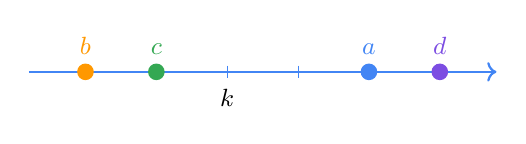
\begin{tikzpicture}[x=0.9cm]
\draw[->,thick,Navy] (-2.8,0)--(3.8,0);
\foreach \i in {-2,...,3}{\draw[Navy] (\i,0.08)--(\i,-0.08);}
\node[below,font=\small] at (0,-0.1){$k$};
\foreach \i/\l/\c in {-2/b/tmOrange,-1/c/tmGreen,2/a/tmBlue,3/d/tmPurple}{\fill[\c] (\i,0) circle (3pt); \node[above,font=\small\bfseries,text=\c] at (\i,0.1){$\l$};}
\end{tikzpicture}\end{center}
\begin{warnbox}Seeing the minus sign in ``$a-2$'', many students think $a$ is small. But $a$ has to \emph{lose} $2$ to equal $k$, so $a$ is bigger than $k$. On the other hand, $b$ has to \emph{gain} $2$ to equal $k$, so $b$ is smaller than $k$.\end{warnbox}
\verify{Try $k=6$ (so that all four numbers are greater than $3$): $a=8$, $b=4$, $c=5$, $d=9$. Then $\dfrac{1}{8-2}=\dfrac{1}{4+2}=\dfrac{1}{5+1}=\dfrac{1}{9-3}=\dfrac{1}{6}$ and indeed $4<5<8<9$, that is, $b<c<a<d$.}
The ordering $b<c<a<d$ is option \textbf{(E)}.
\ans{(E) $b<c<a<d$}
}

% ---------------------------------------------------------------- Problem 13
\begin{probbox}{13}{\relax}
A rectangle has length $x$ and width $y$. A triangle has base $16$ and corresponding height $x$.
If the area of the rectangle equals the area of the triangle, then the value of $y$ is
\choices{$16$}{$4$}{$8$}{$12$}{$32$}
\end{probbox}
\probsol{
\textbf{Understanding the problem.} Rectangle: length $x$, width $y$. Triangle: base $16$, height $x$. The two areas are equal. Find $y$
(note: $x$ is not given, but we will see that $x$ ``disappears'').
\begin{figC}
\draw[tmBlue,line width=1pt,fill=tmBlue!10] (0,0) rectangle (2.4,1.4);
\node[below] at (1.2,0){$x$}; \node[left] at (0,0.7){$y$};
\draw[tmOrange!85!black,line width=1pt,fill=tmOrange!12] (3.6,0)--(7.6,0)--(4.6,2.4)--cycle;
\draw[dashed,Slate] (4.6,2.4)--(4.6,0); \draw[Slate] (4.6,0.18)--(4.78,0.18)--(4.78,0);
\node[below] at (5.6,0){$16$}; \node[left,font=\small] at (4.6,1.1){$x$};
\end{figC}
\step{1}{Write the two area formulas}
\begin{recallbox}Area of a rectangle $=$ length $\times$ width. Area of a triangle $=\dfrac{\text{base}\times\text{height}}{2}$.\end{recallbox}
Rectangle: $A_1=x\cdot y=xy$.\quad Triangle: $A_2=\dfrac{16\cdot x}{2}=8x$.
\step{2}{Write an equation and solve}
$xy=8x$. Since $x$ is a length, $x>0$; dividing both sides by $x$: $y=8$.
\begin{proofbox}You can also see it without dividing: $x\cdot y$ and $x\cdot 8$ are ``$x$ groups of $y$'' and ``$x$ groups of $8$''. If the products are equal with the same number of groups $x\neq 0$, each group must be the same: $y=8$.\end{proofbox}
\begin{warnbox}Forgetting to halve when finding the area of the triangle leads to $y=16$ (option A).\end{warnbox}
\verify{Try $x=5$: rectangle $5\times 8=40$; triangle $\dfrac{16\cdot 5}{2}=40$. Equal. (It works for any $x$.)}
So the answer is \textbf{(C)}.
\ans{(C) $8$}
}

% ---------------------------------------------------------------- Problem 14
\begin{probbox}{14}{\relax}
The symbol \aeaBox{3}{4}{5}{6} is evaluated as $3\times 6+4\times 5=38$. If \aeaBox{2}{6}{1}{\ } is evaluated as $16$,
then the number that should be placed in the empty space is
\choices{$1$}{$2$}{$3$}{$4$}{$5$}
\end{probbox}
\probsol{
\textbf{Understanding the problem.} First we must understand the rule from the given example, then apply it to the box with the unknown number.
\step{1}{Find the rule}
In \aeaBox{3}{4}{5}{6}: $3$ (top left) times $6$ (bottom right), plus $4$ (top right) times $5$ (bottom left): $3\times 6+4\times 5=18+20=38$.
That is: \emph{multiply the two numbers on each diagonal, then add}. In general, \aeaBox{a}{b}{c}{d} $=a\times d+b\times c$.
\step{2}{Name the empty space and write an equation}
Let the number in the empty space (bottom right) be $x$. By the rule: \aeaBox{2}{6}{1}{x} $=2\times x+6\times 1=2x+6$.
We are told the value is $16$: $2x+6=16$.
\step{3}{Solve}
Subtract $6$ from both sides: $2x=10$. Divide both sides by $2$: $x=5$.
\verify{$2\times 5+6\times 1=10+6=16$. Correct.}
\begin{warnbox}Do not pair the wrong numbers: $2\times 6+1\times x$ (multiplying along rows) breaks the rule; that way you would get $x=4$ (option D). Check the rule against the example $38$ before using it.\end{warnbox}
So the answer is \textbf{(E)}.
\begin{parentbox}Together with your child, ``invent'' a new symbol (for example, multiply along the rows and then subtract) and quiz each other. The important habit is always to test a rule on the given example before using it.\end{parentbox}
\ans{(E) $5$}
}

% ---------------------------------------------------------------- Problem 15
\begin{probbox}{15}{\relax}
Three pumpkins are weighed two at a time in all possible ways. The weights of the pairs are $12$ kg, $13$ kg and $15$ kg.
How much does the lightest pumpkin weigh?
\choices{$4$ kg}{$5$ kg}{$6$ kg}{$7$ kg}{$8$ kg}
\end{probbox}
\probsol{
\textbf{Understanding the problem.} Three pumpkins can be paired in exactly $3$ ways. Let their weights from lightest to heaviest be $a\le b\le c$ (kg).
The lightest pair is the two lightest pumpkins, and the heaviest pair is the two heaviest pumpkins:
$a+b=12$, \ $a+c=13$, \ $b+c=15$.
\step{1}{Add all three pairs}
Each pumpkin appears in exactly \emph{two} pairs: $(a+b)+(a+c)+(b+c)=12+13+15=40$, that is, $2(a+b+c)=40$.
\begin{recallbox}Three objects weighed in pairs: the total of the three objects is half of the sum of the results.\end{recallbox}
\step{2}{Total weight of the three pumpkins}
$a+b+c=40\div 2=20$ (kg).
\step{3}{Find the lightest pumpkin}
The lightest pumpkin $a$ is the one that is \emph{not} in the heaviest pair ($b+c=15$):
$a=(a+b+c)-(b+c)=20-15=5$ (kg).
(Similarly: $b=20-13=7$ kg, \ $c=20-12=8$ kg.)
\begin{barfigC}
\blk{0}{1.25}{0}{0.5}{tmGreen}{a}
\blk{1.25}{3}{0}{0.5}{tmOrange}{b}
\brcup{0}{3}{0.5}{12 kg}
\blk{0}{1.25}{-0.9}{0.5}{tmGreen}{a}
\blk{1.25}{3.25}{-0.9}{0.5}{tmPurple}{c}
\brcdn{0}{3.25}{-1.35}{13 kg}
\end{barfigC}
\verify{$5+7=12$, \ $5+8=13$, \ $7+8=15$. All three pairs are correct.}
\begin{warnbox}Do not take $12\div 2=6$ kg and assume each pumpkin in the lightest pair weighs $6$ kg: the two pumpkins in a pair need not weigh the same. Option (E) $8$ kg is the \emph{heaviest} pumpkin.\end{warnbox}
The lightest pumpkin weighs $5$ kg, which is option \textbf{(B)}.
\begin{parentbox}Let your child take three objects at home and a scale: weigh them in pairs, add the three results and halve, then compare with putting all three on the scale together. Your child will see for themselves why we divide by $2$.\end{parentbox}
\ans{(B) $5$ kg}
}

% ---------------- part b ----------------
% ===== Topic 1, part b (EN): problems 16-30 =====
% helper shapes for the balance-scale problems (topic-specific prefix \ae...)
% \aeShp{code}{x}{y}: draw shape (T triangle, C circle, S square, D diamond, Q question mark) with lower-left corner at (x,y)
\providecommand{\aeShp}[3]{%
  \if#1T\draw[tmBlue!80!black,line width=0.8pt,fill=tmBlue!18] (#2,#3)--(#2+0.34,#3)--(#2+0.17,#3+0.3)--cycle;\fi
  \if#1C\draw[tmOrange!85!black,line width=0.8pt,fill=tmOrange!22] (#2+0.15,#3+0.15) circle (0.15);\fi
  \if#1S\draw[tmGreen!80!black,line width=0.8pt,fill=tmGreen!18] (#2,#3) rectangle (#2+0.3,#3+0.3);\fi
  \if#1D\draw[tmPurple!85!black,line width=0.8pt,fill=tmPurple!18] (#2+0.13,#3)--(#2+0.26,#3+0.16)--(#2+0.13,#3+0.32)--(#2,#3+0.16)--cycle;\fi
  \if#1Q\node[font=\Large\bfseries,text=Ink,inner sep=0pt,anchor=south] at (#2+0.15,#3) {?};\fi}
\providecommand{\aeTri}{\tikz[baseline=0pt]{\aeShp{T}{0}{0}}}
\providecommand{\aeCir}{\tikz[baseline=0pt]{\aeShp{C}{0}{0}}}
\providecommand{\aeSq}{\tikz[baseline=0pt]{\aeShp{S}{0}{0}}}
\providecommand{\aeDia}{\tikz[baseline=0pt]{\aeShp{D}{0}{0}}}
% \aeRow{list}{xcentre}{y}: a row of shapes (e.g. {T,C}) centred at xcentre, standing on height y
\providecommand{\aeRow}[3]{%
  \foreach \aeS [count=\aeI] in {#1}{\xdef\aeN{\aeI}}%
  \foreach \aeS [count=\aeI] in {#1}{\aeShp{\aeS}{#2-0.19*\aeN+0.38*\aeI-0.36}{#3+0.03}}}
% \aeScale{x}{y}{left list}{right list}: a balanced scale centred at (x,y)
\providecommand{\aeScale}[4]{\begin{scope}[shift={(#1,#2)}]
  \draw[Ink,line width=1pt] (-1.9,0.55)--(-0.5,0.55) (-1.2,0.55)--(-1.2,0.25)--(1.2,0.25)--(1.2,0.55) (0.5,0.55)--(1.9,0.55);
  \draw[Ink,line width=0.9pt,fill=Ink!12] (-0.2,-0.12)--(0,0.25)--(0.2,-0.12)--cycle;
  \aeRow{#3}{-1.2}{0.55}\aeRow{#4}{1.2}{0.55}
\end{scope}}

% ------------------------------------------------------------------ 16
\begin{probbox}{16}{\relax}
Hồng is learning to save money. Today she has $120$ thousand dong in her savings account. From now on, every time she makes a deposit she will add exactly $30$ thousand dong. If Hồng makes $m$ such deposits, which expression correctly gives the amount of money (in thousands of dong) in her account?
\choices{$120+m$}{$30m$}{$30+120m$}{$150m$}{$120+30m$}
\end{probbox}
\probsol{
\textbf{Analysis.} Given: at the start there are $120$ thousand dong; each deposit adds $30$ thousand dong; there are $m$ deposits. Find: an algebraic expression for the total after $m$ deposits.

\step{1}{Try a few concrete values of $m$ to see the pattern}
\begin{center}
\begin{tabular}{|c|c|c|}
\hline
\rowcolor{tmBlue!10}\textbf{Deposits} & \textbf{Money added} & \textbf{Total (thousand dong)}\\ \hline
$0$ & $0$ & $120$\\ \hline
$1$ & $30$ & $120+30=150$\\ \hline
$2$ & $30+30=30\cdot 2=60$ & $120+60=180$\\ \hline
$3$ & $30\cdot 3=90$ & $120+90=210$\\ \hline
$m$ & $30\cdot m=30m$ & $120+30m$\\ \hline
\end{tabular}
\end{center}

\step{2}{Write the expression}
The money \emph{added} after $m$ deposits is $m$ times $30$, that is $30m$. Adding the $120$ already in the account gives
\[ \text{Total} = 120 + 30m \ \text{(thousand dong)}. \]
\begin{recallbox}$30m$ means $30\cdot m$ (we may leave out the multiplication sign between a number and a letter). Adding a number $a$ to itself $m$ times gives $a\cdot m$.\end{recallbox}

\step{3}{Rule out the wrong options}
\begin{itemize}[leftmargin=1.3em,itemsep=1pt]
\item (A) $120+m$: adds only $1$ thousand each time -- wrong.
\item (B) $30m$: forgets the $120$ thousand already there. For $m=0$ it gives $0$ -- wrong.
\item (C) $30+120m$: swaps the roles of the two numbers. For $m=1$ it gives $150$ (the same!), but for $m=2$ it gives $270\ne 180$ -- wrong.
\item (D) $150m$: for $m=2$ it gives $300\ne 180$ -- wrong.
\end{itemize}
\begin{warnbox}Testing only \emph{one} value, $m=1$, is not enough: (C), (D) and (E) all give $150$. Also try $m=0$ or $m=2$ to tell them apart.\end{warnbox}
\verify{For $m=3$: $120+30\cdot 3=210$, exactly as in the table of Step 1.}
So the answer is \textbf{(E)}.
\ans{(E) $120+30m$}
}

% ------------------------------------------------------------------ 17
\begin{probbox}{17}{\relax}
All four scales below are balanced. Identical shapes have equal masses. One possible replacement for the ``?'' that keeps the fourth scale balanced is
\begin{figC}
\aeScale{0}{1.6}{T,C}{S}
\aeScale{4.6}{1.6}{T}{D,C}
\aeScale{0}{0}{D,T}{C,S}
\aeScale{4.6}{0}{C,D,T}{Q}
\node[font=\footnotesize\bfseries,text=Slate] at (-2.25,2.45) {1};
\node[font=\footnotesize\bfseries,text=Slate] at (2.35,2.45) {2};
\node[font=\footnotesize\bfseries,text=Slate] at (-2.25,0.85) {3};
\node[font=\footnotesize\bfseries,text=Slate] at (2.35,0.85) {4};
\end{figC}
\choices{\aeTri\,\aeSq}{\aeDia\,\aeTri}{\aeCir\,\aeSq}{\aeSq\,\aeDia}{\aeTri\,\aeCir}
\end{probbox}
\probsol{
\textbf{Analysis.} Each balanced scale gives an \emph{equation}: the total mass on the left pan equals the total mass on the right pan. We write the shapes straight into the equations (each shape stands for its mass):
\[
\text{Scale 1: } \aeTri+\aeCir=\aeSq,\qquad
\text{Scale 2: } \aeTri=\aeDia+\aeCir,\qquad
\text{Scale 3: } \aeDia+\aeTri=\aeCir+\aeSq.
\]
Find: the right pan of scale 4 must weigh the same as $\aeCir+\aeDia+\aeTri$. Idea: convert every shape into one common ``unit'', namely \aeCir.
\begin{recallbox}If a scale is balanced, then \emph{replacing} an object by objects of the same mass, or \emph{removing} identical objects from both pans, keeps it balanced. This is exactly the property of equations: $a=b \Rightarrow a+c=b+c$ and $a-c=b-c$.\end{recallbox}

\step{1}{Use scale 2 to replace \aeTri\ in scale 1}
By scale 2, $\aeTri=\aeDia+\aeCir$. Substituting into scale 1:
\[ \aeSq=\aeTri+\aeCir=(\aeDia+\aeCir)+\aeCir=\aeDia+2\,\aeCir. \]

\step{2}{Substitute into scale 3 to find \aeDia}
Left pan of scale 3: $\aeDia+\aeTri=\aeDia+(\aeDia+\aeCir)=2\,\aeDia+\aeCir$.\par
Right pan of scale 3: $\aeCir+\aeSq=\aeCir+(\aeDia+2\,\aeCir)=\aeDia+3\,\aeCir$.\par
So $2\,\aeDia+\aeCir=\aeDia+3\,\aeCir$. Remove one \aeDia\ and one \aeCir\ from both pans:
\[ \aeDia = 2\,\aeCir. \]

\step{3}{Express every shape in units of \aeCir}
\[ \aeDia=2\,\aeCir,\qquad \aeTri=\aeDia+\aeCir=3\,\aeCir,\qquad \aeSq=\aeDia+2\,\aeCir=4\,\aeCir. \]
Left pan of scale 4: $\aeCir+\aeDia+\aeTri=1+2+3=6$ (\aeCir).

\step{4}{Work out each option (in units of \aeCir)}
\begin{center}
\begin{tabular}{|c|c|c|c|c|c|}
\hline
\rowcolor{tmBlue!10} & (A) \aeTri\,\aeSq & (B) \aeDia\,\aeTri & (C) \aeCir\,\aeSq & (D) \aeSq\,\aeDia & (E) \aeTri\,\aeCir\\ \hline
Mass & $3+4=7$ & $2+3=5$ & $1+4=5$ & $4+2=\mathbf{6}$ & $3+1=4$\\ \hline
\end{tabular}
\end{center}
Only (D) weighs exactly $6$ \aeCir.
\verify{Let \aeCir\ weigh $1$~kg; then \aeDia, \aeTri, \aeSq\ weigh $2$, $3$, $4$~kg. Scale 1: $3+1=4$ \checkmark; scale 2: $3=2+1$ \checkmark; scale 3: $2+3=1+4$ \checkmark; scale 4: $1+2+3=6=4+2$ \checkmark.}
\begin{tipbox}When there are several unknowns, choose \emph{one} shape as the unit of measurement and express all the others in terms of it -- just like changing all amounts of money into the same kind of banknote.\end{tipbox}
So the answer is \textbf{(D)}.
\ans{(D) \aeSq\,\aeDia}
}

% ------------------------------------------------------------------ 18
\begin{probbox}{18}{\relax}
The number that goes in the box to make $\dfrac{3}{7}=\dfrac{\square}{63}$ true is
\choices{$27$}{$9$}{$59$}{$63$}{$3$}
\end{probbox}
\probsol{
\textbf{Analysis.} Two fractions are equal and the denominator of the second one is $63$. Find its numerator.
\begin{recallbox}\textbf{Basic property of fractions:} multiplying both the numerator and the denominator of a fraction by the same non-zero number gives an equal fraction: $\dfrac{a}{b}=\dfrac{a\cdot k}{b\cdot k}$ $(k\ne 0)$.\end{recallbox}

\step{1}{What was the denominator multiplied by?}
From $7$ to $63$: $63\div 7=9$. So the denominator was multiplied by $9$.

\step{2}{Multiply the numerator by the same number}
To keep the fraction unchanged, the numerator must also be multiplied by $9$: $3\cdot 9=27$.
\[ \frac{3}{7}=\frac{3\cdot 9}{7\cdot 9}=\frac{27}{63}. \]

\step{3}{Another way: ``cross-multiplication''}
$\dfrac{a}{b}=\dfrac{c}{d}$ exactly when $a\cdot d=b\cdot c$. Call the missing number $x$: $3\cdot 63=7\cdot x$, so $189=7x$ and $x=189\div 7=27$.
\begin{warnbox}Some students see $63-7=56$ and then compute $3+56=59$ (option C). A fraction does \emph{not} stay the same when we \emph{add} the same number to its numerator and denominator! We must \emph{multiply} (or divide).\end{warnbox}
\verify{Dividing $27$ and $63$ by $9$ gives $3$ and $7$, so $\dfrac{27}{63}=\dfrac{3}{7}$ \checkmark.}
So the answer is \textbf{(A)}.
\ans{(A) $27$}
}

% ------------------------------------------------------------------ 19
\begin{probbox}{19}{\relax}
The sum of four numbers is $T$. Each of the four numbers is increased by $1$. The four new numbers are added together, and the sum is then multiplied by $3$. The final result is
\choices{$3T+3$}{$3T+4$}{$3T+12$}{$T+12$}{$12T$}
\end{probbox}
\probsol{
\textbf{Analysis.} There are four unknown numbers and we only know their sum is $T$. We do not need each number -- only how the \emph{sum} changes.

\step{1}{Name the numbers}
Call the four numbers $a$, $b$, $c$, $d$. We are told $a+b+c+d=T$.

\step{2}{Increase each number by 1 and add}
The new numbers are $a+1$, $b+1$, $c+1$, $d+1$. Their sum is
\[ (a+1)+(b+1)+(c+1)+(d+1)=(a+b+c+d)+(1+1+1+1)=T+4. \]
\begin{recallbox}Addition is commutative and associative, so we may group the letters together and the numbers together.\end{recallbox}

\step{3}{Multiply by 3}
\[ 3\cdot(T+4)=3\cdot T+3\cdot 4=3T+12. \]
\begin{recallbox}\textbf{Distributive property:} $k\cdot(x+y)=k\cdot x+k\cdot y$. The $3$ must multiply \emph{each} term in the brackets.\end{recallbox}
\begin{warnbox}Two common mistakes: (1) adding only $1$ to the sum (instead of $4$, since there are four numbers), which gives $3T+3$; (2) forgetting to multiply the $4$ by $3$, which gives $3T+4$.\end{warnbox}
\verify{Take the numbers $1,2,3,4$: $T=10$. The new numbers $2,3,4,5$ add to $14$; times $3$ gives $42$. And $3T+12=30+12=42$ \checkmark. The other options give $33$, $34$, $22$, $120$ -- all wrong.}
So the answer is \textbf{(C)}.
\ans{(C) $3T+12$}
}

% ------------------------------------------------------------------ 20
\begin{probbox}{20}{\relax}
Two isosceles triangles each have at least one angle measuring $70^\circ$. In the first triangle, the measure (in degrees) of each of the other two angles is even. In the second triangle, the measure of each of the other two angles is odd. Let $S$ be the sum of the two equal angles of the first triangle and $T$ the sum of the two equal angles of the second triangle. The value of $S+T$ is
\choices{$280^\circ$}{$250^\circ$}{$220^\circ$}{$200^\circ$}{$300^\circ$}
\end{probbox}
\probsol{
\textbf{Analysis.} An isosceles triangle has two equal base angles. The $70^\circ$ angle could be the \emph{apex angle} or a \emph{base angle}. We look at both possibilities and see which one gives ``the other two angles even'' and which one gives ``the other two angles odd''.
\begin{recallbox}The three angles of a triangle add up to $180^\circ$. In an isosceles triangle the two base angles are equal.\end{recallbox}

\step{1}{Possibility 1: the $70^\circ$ angle is a base angle}
Then the other base angle is also $70^\circ$. The apex angle is $180^\circ-70^\circ-70^\circ=40^\circ$.\par
The angles are $70^\circ,\ 70^\circ,\ 40^\circ$. The other two angles (apart from one $70^\circ$ angle) are $70^\circ$ and $40^\circ$ -- \textbf{both even}.

\step{2}{Possibility 2: the $70^\circ$ angle is the apex angle}
The two base angles are equal and add up to $180^\circ-70^\circ=110^\circ$, so each is $110^\circ\div 2=55^\circ$.\par
The angles are $70^\circ,\ 55^\circ,\ 55^\circ$. The other two angles are $55^\circ$ and $55^\circ$ -- \textbf{both odd}.
\begin{figC}
\begin{scope}
\draw[tmBlue,line width=1.1pt,fill=tmBlue!8] (0,0)--(1.6,0)--(0.8,2.2)--cycle;
\node[font=\scriptsize] at (0.33,0.2) {$70^\circ$};
\node[font=\scriptsize] at (1.27,0.2) {$70^\circ$};
\node[font=\scriptsize] at (0.8,1.65) {$40^\circ$};
\node[font=\footnotesize\bfseries,text=tmBlue] at (0.8,-0.35) {First triangle};
\end{scope}
\begin{scope}[xshift=3.6cm]
\draw[tmOrange,line width=1.1pt,fill=tmOrange!8] (0,0)--(2.4,0)--(1.2,1.71)--cycle;
\node[font=\scriptsize] at (0.45,0.18) {$55^\circ$};
\node[font=\scriptsize] at (1.95,0.18) {$55^\circ$};
\node[font=\scriptsize] at (1.2,1.25) {$70^\circ$};
\node[font=\footnotesize\bfseries,text=tmOrange!85!black] at (1.2,-0.35) {Second triangle};
\end{scope}
\end{figC}

\step{3}{Find $S$ and $T$}
The first triangle (other two angles even) is possibility 1. Its two \emph{equal} angles are the two $70^\circ$ angles: $S=70^\circ+70^\circ=140^\circ$.\par
The second triangle (other two angles odd) is possibility 2. Its two equal angles are the $55^\circ$ angles: $T=55^\circ+55^\circ=110^\circ$.

\step{4}{Compute $S+T$}
$S+T=140^\circ+110^\circ=250^\circ$.
\begin{warnbox}``The sum of the equal angles'' is the sum of the two \emph{base} angles, not the sum of the two ``other'' angles. In the first triangle the other two angles are $70^\circ$ and $40^\circ$ (sum $110^\circ$), but the equal angles are $70^\circ$ and $70^\circ$ (sum $140^\circ$). Mixing these up gives $110^\circ+110^\circ=220^\circ$ (option C).\end{warnbox}
\verify{$70+70+40=180$ and $70+55+55=180$ \checkmark.}
So the answer is \textbf{(B)}.
\ans{(B) $250^\circ$}
}

% ------------------------------------------------------------------ 21
\begin{probbox}{21}{\relax}
Ánh is on a $6$-day kayak trip with a total distance of $168$~km. At the end of the third day she has covered $\frac{3}{7}$ of the total distance. How many kilometres per day must she average for the rest of the trip?
\choices{$29$}{$24$}{$27$}{$32$}{$26$}
\end{probbox}
\probsol{
\textbf{Analysis.} Given: total distance $168$~km; the trip lasts $6$ days; after $3$ days $\frac{3}{7}$ of the distance is done. Find: the average number of km per day for the remaining days.
\begin{recallbox}To find $\frac{m}{n}$ of a number, multiply the number by $\frac{m}{n}$ (divide by $n$, then multiply by $m$).\end{recallbox}

\step{1}{Draw a bar model: split the distance into 7 equal parts}
\begin{barfigC}
\foreach \i in {0,1,2}{\blk{\i*1.3}{\i*1.3+1.3}{0}{0.6}{tmGreen}{}}
\foreach \i in {3,4,5,6}{\blk{\i*1.3}{\i*1.3+1.3}{0}{0.6}{tmOrange}{}}
\brcup{0}{3.9}{0.55}{done: $3$ parts (3 days)}
\brcup{3.9}{9.1}{0.55}{left: $4$ parts (3 days)}
\brcdn{0}{9.1}{-0.55}{$168$ km}
\end{barfigC}
Each part is $168\div 7=24$~km long.

\step{2}{Distance done and distance left}
Done: $3$ parts $=3\cdot 24=72$~km.\par
Left: $168-72=96$~km (or $4$ parts $=4\cdot 24=96$~km).

\step{3}{Days left}
The trip lasts $6$ days and $3$ are over, so $6-3=3$ days remain.

\step{4}{Average per day}
$96\div 3=32$~km per day.
\begin{warnbox}Do not confuse ``the fraction of the distance left'' ($\frac{4}{7}$) with ``the number of days left'' ($3$ days). Option (B), $24$~km, is just the length of \emph{one seventh} of the distance.\end{warnbox}
\verify{$72+3\cdot 32=72+96=168$~km \checkmark.}
So the answer is \textbf{(D)}.
\ans{(D) $32$~km per day}
}

% ------------------------------------------------------------------ 22
\begin{probbox}{22}{\stars{1}}
A dot starts at the point $(20,19)$ of the coordinate plane. On the first move it travels $1$ unit horizontally or vertically, that is, to one of the points $(21,19)$, $(19,19)$, $(20,20)$ or $(20,18)$. On the second move it travels $2$ units (in either direction) \emph{perpendicular} to the first move. From then on, each move is $1$ unit longer than the previous one ($3$ units, $4$ units, $5$ units, \dots) and is always perpendicular to the move just before it. The dot stops after $10$ moves. Which of the following final positions is \textbf{not} possible?
\choices{$(27,33)$}{$(30,40)$}{$(21,21)$}{$(42,44)$}{$(37,37)$}
\end{probbox}
\probsol{
\textbf{Analysis.} The moves have lengths $1,2,3,\dots,10$. ``Perpendicular to the previous move'' means the moves \emph{alternate}: horizontal -- vertical -- horizontal -- vertical\dots\ We must find the point the dot can never reach.
\begin{recallbox}In the coordinate plane, moving right (left) $k$ units increases (decreases) the first coordinate by $k$; moving up (down) $k$ units increases (decreases) the second coordinate by $k$.\end{recallbox}

\step{1}{Split the moves into two groups}
If move $1$ is horizontal, then the horizontal moves are moves $1,3,5,7,9$ (odd lengths) and the vertical moves are moves $2,4,6,8,10$ (even lengths). If move $1$ is vertical, it is the other way round.\par
Each move can go in the positive direction (sign $+$) or the negative direction (sign $-$). So the displacement in one direction is
\[ \pm 1\pm 3\pm 5\pm 7\pm 9 \quad\text{(odd group)},\qquad \pm 2\pm 4\pm 6\pm 8\pm 10\quad\text{(even group).} \]

\step{2}{Which numbers can the odd group give?}
If every sign is $+$: $1+3+5+7+9=25$. Changing the sign of a move of length $a$ from $+$ to $-$ lowers the total by $2a$ (we lose $a$ and then subtract another $a$). Hence
\[ \text{displacement}=25-2\times(\text{sum of the lengths whose sign is changed}). \]
To get $21$, the lengths whose sign is changed must add up to $(25-21)\div 2=2$. But no choice of numbers from $\{1,3,5,7,9\}$ adds up to $2$ (choosing $1$ gives $1$; choosing any further number already gives at least $4$). So \textbf{the odd group cannot give a displacement of $21$} (and likewise not $-21$).
\begin{proofbox}The possible sums of numbers chosen from $\{1,3,5,7,9\}$ are $0,1,3,4,5,6,7,8,9,\dots$ but \emph{not} $2$: the smallest number is $1$ and the next smallest is $3$, so choosing two or more numbers gives at least $1+3=4$.\end{proofbox}

\step{3}{Check option (B) $(30,40)$}
Displacement: horizontal $30-20=10$, vertical $40-19=21$.\par
A signed sum of $5$ odd numbers is always \emph{odd}; a signed sum of even numbers is always \emph{even}. Since $21$ is odd, the vertical direction must be the odd group, so we would need $\pm1\pm3\pm5\pm7\pm9=21$ -- impossible by Step 2. So the dot \textbf{cannot} reach $(30,40)$.

\step{4}{All other options can be reached (show the moves)}
\begin{center}\small
\begin{tabular}{|c|c|c|c|}
\hline
\rowcolor{tmBlue!10}\textbf{Point} & \textbf{Displacement (horiz., vert.)} & \textbf{Odd group} & \textbf{Even group}\\ \hline
(A) $(27,33)$ & $(7,14)$ & $1+3+5+7-9=7$ & $2+4+6-8+10=14$\\ \hline
(C) $(21,21)$ & $(1,2)$ & $1-3+5+7-9=1$ & $2-4+6+8-10=2$\\ \hline
(D) $(42,44)$ & $(22,25)$ & $1+3+5+7+9=25$ & $2-4+6+8+10=22$\\ \hline
(E) $(37,37)$ & $(17,18)$ & $-1-3+5+7+9=17$ & $2+4-6+8+10=18$\\ \hline
\end{tabular}
\end{center}
(In (D) the horizontal displacement $22$ is even, so the first move must be vertical.) For example, a path to $(21,21)$: right $1$, up $2$, left $3$, down $4$, right $5$, up $6$, right $7$, up $8$, left $9$, down $10$:
\begin{figC}\begin{scope}[scale=0.24]
\draw[Line,line width=0.3pt] (-3,-3) grid (11,13);
\draw[tmBlue,line width=1.2pt,->] (0,0)--(1,0)--(1,2)--(-2,2)--(-2,-2)--(3,-2)--(3,4)--(10,4)--(10,12)--(1,12)--(1,2);
\fill[tmGreen] (0,0) circle (7pt); \fill[AnsRed] (1,2) circle (7pt);
\node[font=\scriptsize,anchor=north east] at (0,0) {$(20,19)$};
\node[font=\scriptsize,anchor=west,fill=white,inner sep=1pt] at (1.6,1.1) {$(21,21)$};
\end{scope}\end{figC}
\begin{warnbox}Looking only at even and odd is not enough: both $10$ (even) and $21$ (odd) are ``allowed'' as far as parity goes, yet $21$ still cannot be reached. You must really check whether a choice of signs exists.\end{warnbox}
So the answer is \textbf{(B)}.
\ans{(B) $(30,40)$}
}

% ------------------------------------------------------------------ 23
\begin{probbox}{23}{\relax}
Giang works as a server in a restaurant. On Saturday she gets up at 6:30 a.m., starts work at $x$ a.m. and finishes at $x$ p.m. (the same day). How long does Giang work on Saturday?
\choicesII{$24-2x$ hours}{$12-x$ hours}{$2x$ hours}{$0$ hours}{$12$ hours}
\end{probbox}
\probsol{
\textbf{Analysis.} She starts at $x$ a.m. and finishes at $x$ p.m. Find how long she works. The wake-up time 6:30 a.m. is \emph{extra} information that we do not need.
\begin{recallbox}$x$ p.m. (12-hour clock) is the same as $(x+12)$ o'clock on the 24-hour clock. For example, 3 p.m. is 15:00.\end{recallbox}

\step{1}{Change to the 24-hour clock}
Start: $x$ o'clock. Finish: $(x+12)$ o'clock.

\step{2}{Compute the working time}
Time $=$ finishing time $-$ starting time $=(x+12)-x=12$ hours.

\step{3}{Another way to think (two pieces)}
\begin{figC}
\draw[Navy,line width=1pt,->] (0,0)--(8.4,0);
\foreach \x/\l in {0/{$x$ a.m.},4/{12 noon},8/{$x$ p.m.}}{\draw[Navy,line width=1pt] (\x,0.12)--(\x,-0.12); \node[below,font=\footnotesize] at (\x,-0.12) {\l};}
\brcup{0}{4}{0.25}{$12-x$ hours}
\brcup{4}{8}{0.25}{$x$ hours}
\end{figC}
From $x$ a.m. to 12 noon is $12-x$ hours; from 12 noon to $x$ p.m. is $x$ hours. In total: $(12-x)+x=12$ hours. The result does not depend on $x$!
\begin{warnbox}Option (B) $12-x$ is only the morning part. Option (D) $0$ hours comes from computing $x-x$ and forgetting that one time is ``a.m.'' and the other is ``p.m.''.\end{warnbox}
\verify{If $x=8$: she works from 8 a.m. to 8 p.m. (20:00), that is $20-8=12$ hours \checkmark.}
So the answer is \textbf{(E)}.
\ans{(E) $12$ hours}
}

% ------------------------------------------------------------------ 24
\begin{probbox}{24}{\stars{1}}
An $8\times 8\times n$ rectangular box ($n$ a positive integer) is built from $1\times1\times1$ cubes. Let $A$ be the surface area of the box and $B$ the combined surface area of all the small cubes that make it up. The sum of all values of $n$ for which $\dfrac{B}{A}$ is an integer is
\choices{$86$}{$90$}{$70$}{$78$}{$96$}
\end{probbox}
\probsol{
\textbf{Analysis.} We write $A$ and $B$ in terms of $n$, form the ratio $\frac{B}{A}$, find every positive integer $n$ making it an integer, and finally add those values of $n$.
\begin{figC}\begin{scope}[scale=0.8]
\draw[tmBlue,line width=1pt,fill=tmBlue!10] (0,0) rectangle (2.4,1.6);
\draw[tmBlue,line width=1pt,fill=tmBlue!20] (0,1.6)--(0.9,2.3)--(3.3,2.3)--(2.4,1.6)--cycle;
\draw[tmBlue,line width=1pt,fill=tmBlue!5] (2.4,0)--(3.3,0.7)--(3.3,2.3)--(2.4,1.6)--cycle;
\node[below,font=\footnotesize] at (1.2,0) {$8$};
\node[right,font=\footnotesize] at (3.3,1.5) {$n$};
\node[below right,font=\footnotesize] at (2.8,0.4) {$8$};
\end{scope}\end{figC}
\begin{recallbox}A rectangular box with dimensions $a,b,c$ has surface area (total area of its $6$ faces) $2(ab+bc+ca)$. A unit cube has $6$ faces of area $1$, so its surface area is $6$. An $a\times b\times c$ box is made of $a\cdot b\cdot c$ unit cubes.\end{recallbox}

\step{1}{Compute $A$}
$A=2(8\cdot 8+8\cdot n+8\cdot n)=2(64+16n)=128+32n$.

\step{2}{Compute $B$}
Number of small cubes: $8\cdot 8\cdot n=64n$. Each has surface area $6$, so $B=6\cdot 64n=384n$.

\step{3}{Simplify the ratio}
\[ \frac{B}{A}=\frac{384n}{128+32n}=\frac{32\cdot 12n}{32\cdot(4+n)}=\frac{12n}{n+4}. \]

\step{4}{Split off the whole part}
\[ \frac{12n}{n+4}=\frac{12(n+4)-48}{n+4}=12-\frac{48}{n+4}. \]
\begin{proofbox}$12(n+4)-48=12n+48-48=12n$, so the numerator is unchanged. Therefore $\frac{12n}{n+4}$ is an integer exactly when $\frac{48}{n+4}$ is an integer, that is, when $n+4$ is a divisor of $48$.\end{proofbox}

\step{5}{Find the values of $n$}
The positive divisors of $48$ are $1,2,3,4,6,8,12,16,24,48$. Since $n\ge 1$, we need $n+4\ge 5$; keep only $6,8,12,16,24,48$:
\begin{center}
\begin{tabular}{|c|c|c|c|c|c|c|}
\hline
\rowcolor{tmBlue!10}$n+4$ & $6$ & $8$ & $12$ & $16$ & $24$ & $48$\\ \hline
$n$ & $2$ & $4$ & $8$ & $12$ & $20$ & $44$\\ \hline
$\frac{B}{A}=12-\frac{48}{n+4}$ & $4$ & $6$ & $8$ & $9$ & $10$ & $11$\\ \hline
\end{tabular}
\end{center}

\step{6}{Add the values}
$2+4+8+12+20+44=90$.
\begin{warnbox}Do not forget the condition $n\ge 1$: the divisors $1,2,3,4$ of $48$ give $n+4\le 4$, that is $n\le 0$ -- rejected.\end{warnbox}
\verify{For $n=2$: $A=128+64=192$, $B=768$, $\frac{B}{A}=4$ \checkmark. For $n=44$: $A=128+1408=1536$, $B=16\,896$, $\frac{B}{A}=11$ \checkmark.}
So the answer is \textbf{(B)}.
\ans{(B) $90$}
}

% ------------------------------------------------------------------ 25
\begin{probbox}{25}{\stars{1}}
Three bus routes cross at the stop $X$ as shown (segments with the same number of tick marks have equal length). Every $12$ minutes, bus A completes a trip $P\to X\to S\to X\to P$. Every $20$ minutes, bus B completes a trip $Q\to X\to T\to X\to Q$. Every $28$ minutes, bus C completes a trip $R\to X\to U\to X\to R$. At 1:00 p.m., buses A, B and C leave $P$, $Q$ and $R$ respectively; each bus drives at a constant speed and turns around instantly at the end of its route. The buses run continuously until 11:00 p.m. Between 5:00 p.m. and 10:00 p.m., how many times are two or more buses at $X$ at the same moment?
\begin{figC}
\draw[Ink,line width=1pt] (0,1.6)--(0,-1.6) (-2.2,0)--(2.2,0) (-1.9,-1.4)--(1.9,1.4);
\foreach \p/\q/\l/\a in {(0,1.6)/P/P/above,(0,-1.6)/S/S/below,(-2.2,0)/Q/Q/left,(2.2,0)/T/T/right,(-1.9,-1.4)/R/R/below left,(1.9,1.4)/U/U/above right}{\fill[Ink] \p circle (2pt); \node[\a,font=\small\itshape] at \p {$\l$};}
\fill[Ink] (0,0) circle (2pt); \node[below right,font=\small\itshape] at (0.05,-0.05) {$X$};
\draw[tmBlue,line width=1pt] (-0.12,0.8)--(0.12,0.8) (-0.12,-0.8)--(0.12,-0.8);
\foreach \x in {-1.1,1.1}{\draw[tmOrange,line width=1pt] (\x-0.05,-0.12)--(\x-0.05,0.12) (\x+0.05,-0.12)--(\x+0.05,0.12);}
\foreach \t in {-0.5,0.5}{\begin{scope}[shift={(1.9*\t,1.4*\t)},rotate=36.4]
  \draw[tmGreen,line width=1pt] (-0.09,-0.12)--(-0.09,0.12) (0,-0.12)--(0,0.12) (0.09,-0.12)--(0.09,0.12);\end{scope}}
\end{figC}
\choicesII{$18$}{$19$}{$20$}{$21$}{$22$}
\end{probbox}
\probsol{
\textbf{Analysis.} Each bus runs steadily along a route with two arms of equal length. We find \emph{the times} at which each bus is at $X$, then count the times that coincide. Measure time $t$ as \emph{the number of minutes after 1:00 p.m.}: then 5:00 p.m. corresponds to $t=240$ and 10:00 p.m. to $t=540$.

\step{1}{When is bus A at $X$?}
A trip $P\to X\to S\to X\to P$ consists of $4$ equal segments ($PX=XS$) and takes $12$ minutes, so each segment takes $12\div 4=3$ minutes. Bus A reaches $X$ after $3$ minutes, then goes $X\to S\to X$ in $6$ minutes, so it is at $X$ again at minute $9$; after that at minutes $15, 21, 27,\dots$ That is,
\[ t=3,\ 9,\ 15,\ 21,\dots \quad = 3\times 1,\ 3\times 3,\ 3\times 5,\ 3\times 7,\dots \]
Bus A is at $X$ exactly at the times $t=3\times(\text{odd number})$.

\step{2}{Similarly for buses B and C}
Bus B: each segment takes $20\div 4=5$ minutes; it is at $X$ when $t=5,15,25,\dots=5\times(\text{odd})$.\par
Bus C: each segment takes $28\div 4=7$ minutes; it is at $X$ when $t=7,21,35,\dots=7\times(\text{odd})$.

\step{3}{When are two buses at $X$ together?}
\begin{proofbox}Buses A and B are both at $X$ $\iff$ $t=3\times(\text{odd})=5\times(\text{odd})$. Then $t$ is odd (a product of odd numbers is odd), and $t$ is divisible by both $3$ and $5$, hence by $15$; so $t$ is an \emph{odd multiple of $15$}. Conversely, if $t=15\times(\text{odd})$, then $t=3\times(5\times\text{odd})=5\times(3\times\text{odd})$, where the brackets are odd, so both buses are at $X$.\end{proofbox}
By exactly the same argument: A and C are at $X$ together $\iff$ $t$ is an odd multiple of $21$; B and C $\iff$ $t$ is an odd multiple of $35$; all three buses $\iff$ $t$ is an odd multiple of $105$.
\begin{recallbox}If a number is divisible by two coprime numbers $a$ and $b$, then it is divisible by $a\cdot b$. For example: divisible by $3$ and by $5$ implies divisible by $15$.\end{recallbox}

\step{4}{Count in the range $240\le t\le 540$}
\begin{itemize}[leftmargin=1.3em,itemsep=1pt]
\item Odd multiples of $15$: $15\times 17=255$, \dots, $15\times 35=525$ (for $17,19,\dots,35$): \textbf{10} times.
\item Odd multiples of $21$: $21\times 13=273$, \dots, $21\times 25=525$ (for $13,15,\dots,25$): \textbf{7} times.
\item Odd multiples of $35$: $35\times 7=245$, \dots, $35\times 15=525$ (for $7,9,\dots,15$): \textbf{5} times.
\item Odd multiples of $105$: $105\times 3=315$ and $105\times 5=525$: \textbf{2} times (all three buses).
\end{itemize}

\step{5}{Remove the double counting}
At $t=315$ and $t=525$ all three buses are at $X$, so each of these times was counted \emph{three times} in $10+7+5=22$ (once in each list), although it should be counted once. We subtract $2$ for each of them:
\[ 22-2\times 2=18. \]
The full list of the $18$ times (converted to clock times):
\begin{center}\small
\begin{tabular}{|c|c||c|c||c|c|}
\hline
\rowcolor{tmBlue!10}Time & Buses & Time & Buses & Time & Buses\\ \hline
5:05 p.m. & B, C & 6:57 p.m. & A, C & 8:21 p.m. & A, C\\ \hline
5:15 p.m. & A, B & 7:15 p.m. & A, B & 8:35 p.m. & B, C\\ \hline
5:33 p.m. & A, C & 7:25 p.m. & B, C & 8:45 p.m. & A, B\\ \hline
5:45 p.m. & A, B & 7:39 p.m. & A, C & 9:03 p.m. & A, C\\ \hline
\textbf{6:15 p.m.} & \textbf{A, B, C} & 7:45 p.m. & A, B & 9:15 p.m. & A, B\\ \hline
6:45 p.m. & A, B & 8:15 p.m. & A, B & \textbf{9:45 p.m.} & \textbf{A, B, C}\\ \hline
\end{tabular}
\end{center}
\begin{warnbox}Bus A is at $X$ \emph{twice} in every $12$-minute trip (on the way out and on the way back), so the gap between visits is $6$ minutes, not $12$ minutes. Using only ``multiples of $12$, $20$, $28$'' gives a wrong answer.\end{warnbox}
\verify{Checking minute by minute from $240$ to $540$ (for example with a computer) also gives exactly $18$ times.}
So the answer is \textbf{(A)}.
\ans{(A) $18$}
}

% ------------------------------------------------------------------ 26
\begin{probbox}{26}{\relax}
Sơn starts at $7$ and counts forward by $3$, getting the list $7, 10, 13,\dots$ Dũng starts at $2026$ and counts backward by $5$, getting the list $2026, 2021, 2016,\dots$ Which of the following numbers appears in both lists?
\choices{$1009$}{$1006$}{$1003$}{$1001$}{$1011$}
\end{probbox}
\probsol{
\textbf{Analysis.} Each list consists of equally spaced numbers. We find a ``test'' for a number to belong to each list, then check each option.

\step{1}{The test for Sơn's list}
$7=2\cdot 3+1$ leaves remainder $1$ when divided by $3$. Each time we add $3$, the remainder on division by $3$ does not change. So every number in Sơn's list \textbf{leaves remainder $1$ on division by $3$} (and is $\ge 7$). Conversely, every number $\ge 7$ with remainder $1$ appears, since it equals $7+3k$.

\step{2}{The test for Dũng's list}
$2026=405\cdot 5+1$ leaves remainder $1$ on division by $5$. Subtracting $5$ does not change the remainder on division by $5$. So every number in Dũng's list \textbf{leaves remainder $1$ on division by $5$} (and is $\le 2026$), that is, it \textbf{ends in the digit $1$ or $6$}.
\begin{recallbox}Adding or subtracting a multiple of $m$ does not change the remainder on division by $m$. A number leaves remainder $1$ on division by $5$ exactly when its last digit is $1$ or $6$. A number and the sum of its digits leave the same remainder on division by $3$.\end{recallbox}

\step{3}{Check each option}
\begin{center}
\begin{tabular}{|c|c|c|c|}
\hline
\rowcolor{tmBlue!10}\textbf{Number} & \textbf{Digit sum; remainder mod 3} & \textbf{Last digit} & \textbf{In both?}\\ \hline
$1009$ & $10$; rem. $1$ \checkmark & $9$ $\times$ & no\\ \hline
$1006$ & $7$; rem. $1$ \checkmark & $6$ \checkmark & \textbf{yes}\\ \hline
$1003$ & $4$; rem. $1$ \checkmark & $3$ $\times$ & no\\ \hline
$1001$ & $2$; rem. $2$ $\times$ & $1$ \checkmark & no\\ \hline
$1011$ & $3$; rem. $0$ $\times$ & $1$ \checkmark & no\\ \hline
\end{tabular}
\end{center}
\verify{$1006=7+3\cdot 333$ (since $1006-7=999=3\cdot 333$), so $1006$ is the $334$th number in Sơn's list. $2026-1006=1020=5\cdot 204$, so $1006$ is in Dũng's list (after $204$ steps of $5$) \checkmark.}
\begin{tipbox}Instead of writing out hundreds of numbers from each list, we only need the remainder -- a common ``signature'' of every number in the list.\end{tipbox}
So the answer is \textbf{(B)}.
\ans{(B) $1006$}
}

% ------------------------------------------------------------------ 27
\begin{probbox}{27}{\stars{1}}
On a circular track, An stands at point $A$ and Bình stands at point $B$ directly opposite $A$ (segment $AB$ is a diameter). An runs counterclockwise and Bình runs clockwise. They run at constant but different speeds. After a while they notice that every time they pass each other, it is always at the same three places on the track. The ratio of their speeds is
\begin{figC}
\draw[Ink,line width=1.1pt] (0,0) circle (1.1);
\fill[Ink] (0,1.1) circle (2pt) node[above right,font=\small\itshape] {$A$};
\fill[Ink] (0,-1.1) circle (2pt) node[below right,font=\small\itshape] {$B$};
\draw[tmBlue,line width=1pt,->] (-0.2,1.33)--(-0.75,1.18);
\draw[tmOrange,line width=1pt,->] (-0.2,-1.33)--(-0.75,-1.18);
\node[font=\scriptsize,text=tmBlue] at (-1.25,1.45) {An};
\node[font=\scriptsize,text=tmOrange!85!black] at (-1.3,-1.45) {Bình};
\end{figC}
\choicesII{$3:2$}{$3:1$}{$4:1$}{$2:1$}{$5:2$}
\end{probbox}
\probsol{
\textbf{Analysis.} The two friends run \emph{in opposite directions} around the circle. We find what fraction of a lap each one runs between two consecutive meetings, and deduce how many different meeting points there are.

\step{1}{Between two consecutive meetings, together they run exactly 1 lap}
\begin{proofbox}Just after meeting, the two separate in opposite directions. The distance between them (measured along the track) grows, and they meet again when the total distance the two have run just covers the whole circle. So between two consecutive meetings, the \emph{total} distance they run is exactly $1$ lap. (For the first meeting only: they start half a lap apart, so the total is $\frac12$ lap.)\end{proofbox}

\step{2}{What fraction of a lap does An run each time?}
In the same amount of time, distance is proportional to speed. If the ratio of speeds An : Bình is $p:q$, then during $1$ shared lap An runs $\dfrac{p}{p+q}$ of a lap and Bình runs $\dfrac{q}{p+q}$ of a lap.
\begin{recallbox}Sharing a quantity in the ratio $p:q$: the first share is $\frac{p}{p+q}$ and the second share is $\frac{q}{p+q}$ of the total.\end{recallbox}
So each meeting point is an arc of $\dfrac{p}{p+q}$ lap away from the previous one (in An's direction).

\step{3}{Try the ratio $2:1$}
Each time An runs $\frac{2}{3}$ of a lap. Let $M_1$ be the first meeting point. The next meeting points are $\frac23$, $\frac43$, $\frac63=2$ laps, \dots\ away from $M_1$. Since a full lap brings you back to the same place, $\frac43$ lap is the same as $\frac13$ lap, and $2$ laps is $M_1$ itself. There are only \textbf{three} meeting points: $M_1$ and the two points that divide the circle into three equal parts with it. (If Bình is faster, ratio $1:2$, the result is the same.)

\step{4}{How many points do the other ratios give?}
\begin{center}
\begin{tabular}{|c|c|c|c|}
\hline
\rowcolor{tmBlue!10}\textbf{Ratio} & \textbf{An runs each time} & \textbf{Meeting points (measured from $M_1$)} & \textbf{Points}\\ \hline
(A) $3:2$ & $\frac35$ lap & $0,\frac35,\frac15,\frac45,\frac25$ then repeats & $5$\\ \hline
(B) $3:1$ & $\frac34$ lap & $0,\frac34,\frac24,\frac14$ then repeats & $4$\\ \hline
(C) $4:1$ & $\frac45$ lap & $0,\frac45,\frac35,\frac25,\frac15$ & $5$\\ \hline
(D) $2:1$ & $\frac23$ lap & $0,\frac23,\frac13$ & $\mathbf{3}$\\ \hline
(E) $5:2$ & $\frac57$ lap & $7$ different places & $7$\\ \hline
\end{tabular}
\end{center}
(For example, row (A): $\frac35+\frac35=\frac65$, remove $1$ lap to get $\frac15$; add $\frac35$ to get $\frac45$; add $\frac35$ to get $\frac75$, remove $1$ lap to get $\frac25$; add $\frac35$ to get $1$ lap -- back at $M_1$.)
\begin{figC}
\draw[Ink,line width=1.1pt] (0,0) circle (1.1);
\fill[Ink] (0,1.1) circle (2pt) node[above,font=\small\itshape] {$A$};
\fill[Ink] (0,-1.1) circle (2pt) node[below,font=\small\itshape] {$B$};
\foreach \a in {90,210,330}{\fill[AnsRed] (\a:1.1) circle (3pt);}
\node[font=\scriptsize,text=AnsRed,anchor=east] at (210:1.25) {meet};
\node[font=\scriptsize,text=AnsRed,anchor=west] at (330:1.25) {meet};
\node[font=\scriptsize,text=AnsRed,anchor=south west] at (90:1.18) {meet};
\end{figC}
\verify{Let the track be $600$~m long, An run $200$~m per minute and Bình $100$~m per minute. They start $300$~m apart and first meet after $300\div 300=1$ minute, at the point $200$~m from $A$ (in An's direction). After that they meet every $600\div 300=2$ minutes, and An runs another $400$~m each time: positions $200\to 600$ (that is, $A$) $\to 1000$ (that is, $400$~m) $\to 1400$ (that is, $200$~m) \dots\ Exactly three points: $0$~m, $200$~m, $400$~m, dividing the circle into three equal parts -- as in the picture above.}
So the answer is \textbf{(D)}.
\ans{(D) $2:1$}
}

% ------------------------------------------------------------------ 28
\begin{probbox}{28}{\stars{1}}
The list $11, 20, 31, 51, 82$ is an example of an increasing list of five positive integers in which the first and second numbers add to the third, the second and third add to the fourth, and the third and fourth add to the fifth. How many such lists have $124$ as the fifth number?
\choices{$10$}{$7$}{$9$}{$6$}{$8$}
\end{probbox}
\probsol{
\textbf{Analysis.} The whole list is completely determined by its first two numbers. We express the fifth number in terms of the first two, then count the pairs that work.

\step{1}{Express the whole list in terms of the first two numbers $a$ and $b$}
\begin{center}
\begin{tabular}{|c|c|c|c|c|}
\hline
\rowcolor{tmBlue!10}1st & 2nd & 3rd & 4th & 5th\\ \hline
$a$ & $b$ & $a+b$ & $b+(a+b)=a+2b$ & $(a+b)+(a+2b)=2a+3b$\\ \hline
\end{tabular}
\end{center}
Check with the example: $a=11$, $b=20$ gives the fifth number $2\cdot 11+3\cdot 20=22+60=82$ \checkmark.

\step{2}{Conditions}
\begin{itemize}[leftmargin=1.3em,itemsep=1pt]
\item The fifth number is $124$: $2a+3b=124$.
\item $a, b$ are positive integers.
\item The list is increasing: we need $a<b$. (The later steps increase automatically: $a+b>b$, $a+2b>a+b$, \dots\ since $a,b>0$.)
\end{itemize}

\step{3}{$b$ must be even}
$2a$ and $124$ are both even, so $3b=124-2a$ is even, hence $b$ is even. Write $b=2t$ ($t$ a positive integer). Then $2a=124-6t$, that is,
\[ a=62-3t. \]

\step{4}{Find the range of $t$}
\begin{itemize}[leftmargin=1.3em,itemsep=1pt]
\item $a\ge 1$: $62-3t\ge 1 \Rightarrow 3t\le 61 \Rightarrow t\le 20$.
\item $a<b$: $62-3t<2t \Rightarrow 62<5t \Rightarrow t>12.4 \Rightarrow t\ge 13$.
\end{itemize}
So $t\in\{13,14,15,16,17,18,19,20\}$: $8$ values.

\step{5}{List them to check}
\begin{center}\small
\begin{tabular}{|c|c|c|c|c|c|c|c|c|}
\hline
\rowcolor{tmBlue!10}$t$ & $13$ & $14$ & $15$ & $16$ & $17$ & $18$ & $19$ & $20$\\ \hline
$a=62-3t$ & $23$ & $20$ & $17$ & $14$ & $11$ & $8$ & $5$ & $2$\\ \hline
$b=2t$ & $26$ & $28$ & $30$ & $32$ & $34$ & $36$ & $38$ & $40$\\ \hline
\end{tabular}
\end{center}
For example $t=13$: the list $23, 26, 49, 75, 124$; $t=20$: the list $2, 40, 42, 82, 124$.
\begin{warnbox}If we forget the condition ``increasing'' ($a<b$), we overcount pairs such as $a=26$, $b=24$ (the list $26, 24, 50, 74, 124$ -- it decreases at the first step).\end{warnbox}
\verify{$t=12$ gives $a=26$, $b=24$: $a>b$, rejected. $t=21$ gives $a=-1$: not positive, rejected. So there are exactly $8$ lists.}
So the answer is \textbf{(E)}.
\ans{(E) $8$}
}

% ------------------------------------------------------------------ 29
\begin{probbox}{29}{\relax}
Khánh owns more cats than Lan and more dogs than Bảo. Lan owns more dogs than Khánh but fewer cats than Bảo. Which of the following statements \textbf{must} be true?
\choicesL{Bảo owns the fewest cats.}{Bảo owns the most cats.}{Khánh owns the most cats.}{Lan owns the most dogs.}{Khánh owns the fewest dogs.}
\end{probbox}
\probsol{
\textbf{Analysis.} There are two separate kinds of comparison: comparing numbers of \emph{cats} and comparing numbers of \emph{dogs}. We split the information into two groups and put each in order.

\step{1}{Information about cats}
``Khánh owns more cats than Lan'': Lan $<$ Khánh.\quad ``Lan owns fewer cats than Bảo'': Lan $<$ Bảo.\par
So Lan has the fewest cats. But between Khánh and Bảo, \emph{we do not know who has more}.

\step{2}{Information about dogs}
``Khánh owns more dogs than Bảo'': Bảo $<$ Khánh.\quad ``Lan owns more dogs than Khánh'': Khánh $<$ Lan.\par
Together: Bảo $<$ Khánh $<$ Lan. So \textbf{Lan has the most dogs}, and Bảo the fewest dogs.
\begin{figC}
\node[font=\small\bfseries,text=tmOrange!85!black] at (-0.6,1.4) {Cats};
\node[draw=tmOrange,rounded corners=3pt,font=\small] (L) at (1,1.4) {Lan};
\node[draw=tmOrange,rounded corners=3pt,font=\small] (K) at (3,1.9) {Khánh};
\node[draw=tmOrange,rounded corners=3pt,font=\small] (B) at (3,0.9) {Bảo};
\draw[->,tmOrange,line width=0.9pt] (L)--(K); \draw[->,tmOrange,line width=0.9pt] (L)--(B);
\node[font=\scriptsize,text=Slate] at (4.6,1.4) {(cannot compare)};
\node[font=\small\bfseries,text=tmBlue] at (-0.6,0) {Dogs};
\node[draw=tmBlue,rounded corners=3pt,font=\small] (b) at (1,0) {Bảo};
\node[draw=tmBlue,rounded corners=3pt,font=\small] (k) at (3,0) {Khánh};
\node[draw=tmBlue,rounded corners=3pt,font=\small] (l) at (5,0) {Lan};
\draw[->,tmBlue,line width=0.9pt] (b)--(k); \draw[->,tmBlue,line width=0.9pt] (k)--(l);
\node[font=\scriptsize,text=Slate] at (3,-0.55) {arrows point from fewer to more};
\end{figC}

\step{3}{Examine each statement}
\begin{itemize}[leftmargin=1.3em,itemsep=1pt]
\item (A) ``Bảo owns the fewest cats'': \textbf{false}, because Lan has fewer cats than Bảo.
\item (B) ``Bảo owns the most cats'': \emph{may} be true, but not necessarily. For example, Lan $1$, Khánh $3$, Bảo $2$ cats satisfies every condition, yet Khánh has the most cats.
\item (C) ``Khánh owns the most cats'': not necessarily either. For example, with Lan $1$, Khánh $2$, Bảo $3$ cats, Bảo has the most.
\item (D) ``Lan owns the most dogs'': \textbf{must be true} (Step 2).
\item (E) ``Khánh owns the fewest dogs'': \textbf{false}, because Bảo has fewer dogs than Khánh.
\end{itemize}
\begin{warnbox}``Must be true'' means true in \emph{every} situation that fits the problem. Finding a single situation in which a statement is false is enough to reject it.\end{warnbox}
So the answer is \textbf{(D)}.
\ans{(D) Lan owns the most dogs}
}

% ------------------------------------------------------------------ 30
\begin{probbox}{30}{\relax}
Linh bought $300$~g of candy A for $50$ thousand dong and $x$~g of candy B for $70$ thousand dong. She worked out that the average price of all the candy she bought was $15$ thousand dong per $100$~g. What is the value of $x$?
\choices{$525$}{$600$}{$500$}{$450$}{$900$}
\end{probbox}
\probsol{
\textbf{Analysis.} Given: the amounts paid for the two kinds of candy and the average price. Find: the mass of candy B. Idea: from the total cost and the average price, find the \emph{total mass}.
\begin{recallbox}Average price $=$ total cost $\div$ total mass. Therefore total mass $=$ total cost $\div$ average price.\end{recallbox}

\step{1}{Total cost}
$50+70=120$ thousand dong.

\step{2}{Total mass}
Every $100$~g costs $15$ thousand dong. With $120$ thousand dong one can buy $120\div 15=8$ ``portions of $100$ g''. So the total mass is $8\cdot 100=800$~g.

\step{3}{Mass of candy B}
$x=800-300=500$~g.
\begin{center}
\begin{tabular}{|c|c|c|c|}
\hline
\rowcolor{tmBlue!10} & \textbf{Candy A} & \textbf{Candy B} & \textbf{Both}\\ \hline
Mass (g) & $300$ & $x=500$ & $800$\\ \hline
Cost (thousand dong) & $50$ & $70$ & $120$\\ \hline
Price per $100$~g (thousand dong) & $\approx 16.7$ & $14$ & $15$\\ \hline
\end{tabular}
\end{center}
\begin{warnbox}You cannot simply take the average of the two prices ($16.7$ and $14$), because the two masses are different. The average price must be computed as \emph{total cost divided by total mass}.\end{warnbox}
\verify{$120$ thousand dong for $800$~g means $120\div 8=15$ thousand dong per $100$~g \checkmark.}
So the answer is \textbf{(C)}.
\ans{(C) $500$}
}

% ---------------- part c ----------------
% ===================== Topic 1 -- Algebra and Equations -- part c (EN): Problems 31--40 =====================
\providecommand{\aeaBox}[4]{\begin{tikzpicture}[baseline=-0.7ex,font=\small]
  \draw[Navy,line width=0.8pt,fill=tmBlue!6] (-0.66,-0.32) rectangle (0.66,0.32);
  \draw[Navy,line width=0.8pt] (0,-0.32)--(0,0.32) (-0.66,0)--(0.66,0);
  \node[inner sep=0pt] at (-0.33,0.16){$#1$};\node[inner sep=0pt] at (0.33,0.16){$#2$};
  \node[inner sep=0pt] at (-0.33,-0.16){$#3$};\node[inner sep=0pt] at (0.33,-0.16){$#4$};\end{tikzpicture}}

\clearpage
\dividerbar{Extension and challenge}

% ---------------------------------------------------------------- Problem 31
\begin{probbox}{31}{\relax}
The road from Mr Ba's home to the city is $180$ km long. He rides a motorbike at a constant speed, and after $3$ hours he has covered
$\dfrac{2}{3}$ of the distance.
\begin{enumerate}[label=\alph*),leftmargin=1.6em,itemsep=1pt,topsep=2pt]
\item Find the speed of the motorbike.
\item If he keeps the same speed, how much longer will it take him to reach the city?
\item If he wants to arrive $30$ minutes earlier than planned in part b), at what speed must he ride for the rest of the way?
\end{enumerate}
\end{probbox}
\probsol{
\textbf{Understanding the problem.} \emph{Given:} the whole distance $180$ km; in $3$ hours he covered $\dfrac{2}{3}$ of it.
\emph{Find:} the speed; the remaining time; the new speed needed to save $30$ minutes.
\begin{recallbox}$s=v\cdot t$;\quad $v=\dfrac{s}{t}$;\quad $t=\dfrac{s}{v}$. \ \ $\dfrac{m}{n}$ of $A$ equals $A\div n\cdot m$.\end{recallbox}
\step{1}{Distance covered and distance left}
Covered: $\dfrac{2}{3}$ of $180$ km is $180\div 3\cdot 2=60\cdot 2=120$ (km). Left: $180-120=60$ (km).
\begin{barfigC}
\blk{0}{2}{0}{0.55}{tmBlue}{60 km}
\blk{2}{4}{0}{0.55}{tmBlue}{60 km}
\blk{4}{6}{0}{0.55}{tmOrange}{60 km}
\brcup{0}{4}{0.55}{covered (3 hours)}
\brcdn{4}{6}{-0.55}{left}
\end{barfigC}
\step{2}{Part a: the speed}
$v=120\div 3=40$ (km/h).
\step{3}{Part b: the time left}
$t=60\div 40=1.5$ (hours) $=1$ hour $30$ minutes.
\begin{tipbox}Look at the diagram: in $3$ hours he covered $2$ equal parts, so each part takes $1.5$ hours. Exactly $1$ part is left, so it takes $1.5$ hours. You get the answer even without the speed!\end{tipbox}
\step{4}{Part c: the new speed}
New time: $1$ hour $30$ minutes $-\,30$ minutes $=1$ hour. To cover $60$ km in $1$ hour, the speed must be $60\div 1=60$ (km/h).
\begin{warnbox}Do not just add to the speed, as in ``$30$ minutes earlier means $30$ km/h faster''. Recalculate: speed $=$ distance $\div$ new time.\end{warnbox}
\verify{$40\cdot 3=120$ km; $40\cdot 1.5=60$ km; $60\cdot 1=60$ km. Total $120+60=180$ km.}
\ans{a) $40$ km/h;\ \ b) $1$ hour $30$ minutes;\ \ c) $60$ km/h.}
}

% ---------------------------------------------------------------- Problem 32
\begin{probbox}{32}{\relax}
An isosceles triangle has a base of $10$ cm and two equal sides of $2x$ cm each. A rectangle has length $(x+7)$ cm and width $5$ cm.
The perimeter of the triangle equals the perimeter of the rectangle.
\begin{figC}
\draw[tmBlue,line width=1.1pt,fill=tmBlue!10] (0,0)--(2.4,0)--(1.2,2.6)--cycle;
\node[below] at (1.2,0){$10$ cm};
\node[left] at (0.5,1.35){$2x$};\node[right] at (1.9,1.35){$2x$};
\draw[tmBlue,line width=0.9pt] (0.48,1.4)--(0.72,1.2); \draw[tmBlue,line width=0.9pt] (1.68,1.2)--(1.92,1.4);
\draw[tmOrange!85!black,line width=1.1pt,fill=tmOrange!12] (3.6,0) rectangle (7.2,1.3);
\node[below] at (5.4,0){$x+7$}; \node[right] at (7.2,0.65){$5$ cm};
\end{figC}
\begin{enumerate}[label=\alph*),leftmargin=1.6em,itemsep=1pt,topsep=2pt]
\item Write an expression in $x$ for the perimeter of each shape.
\item Find $x$, then find the side lengths of the triangle and the area of the rectangle.
\end{enumerate}
\end{probbox}
\probsol{
\textbf{Understanding the problem.} The triangle has sides $2x$, $2x$, $10$ (cm). The rectangle measures $x+7$ by $5$ (cm). The two perimeters are equal.
\begin{recallbox}Perimeter of a triangle $=$ sum of the three sides. Perimeter of a rectangle $=2\times(\text{length}+\text{width})$. Area of a rectangle $=$ length $\times$ width.\end{recallbox}
\step{1}{Part a: expressions for the perimeters}
Triangle: $2x+2x+10=4x+10$ (cm).\quad Rectangle: $2\cdot\big((x+7)+5\big)=2(x+12)=2x+24$ (cm).
\begin{warnbox}When multiplying the bracket by $2$, multiply both terms: $2(x+12)=2x+24$, not $2x+12$.\end{warnbox}
\step{2}{Part b: write an equation}
$4x+10=2x+24$.
\step{3}{Solve the equation}
Subtract $2x$ from both sides: $2x+10=24$. Subtract $10$ from both sides: $2x=14$. Divide by $2$: $x=7$.
\step{4}{Work out what is asked}
Equal sides of the triangle: $2x=14$ cm, so the triangle has sides $14$ cm, $14$ cm, $10$ cm.\\
Rectangle: length $x+7=14$ cm, width $5$ cm, area $14\cdot 5=70$ (cm$^2$).
\verify{Perimeter of the triangle $14+14+10=38$ cm; perimeter of the rectangle $2(14+5)=38$ cm. Equal.}
\ans{a) $4x+10$ and $2x+24$;\ \ b) $x=7$; triangle $14$ cm, $14$ cm, $10$ cm; area of the rectangle $70$ cm$^2$.}
}

% ---------------------------------------------------------------- Problem 33
\begin{probbox}{33}{\stars{1}}
We use the rule of Problem 14 again:\quad \aeaBox{a}{b}{c}{d} $=a\cdot d+b\cdot c$.
\begin{enumerate}[label=\alph*),leftmargin=1.6em,itemsep=2pt,topsep=2pt]
\item Evaluate \aeaBox{-3}{4}{5}{2}.
\item Find $x$ if \aeaBox{x}{2}{3}{4} $=$ \aeaBox{1}{x}{5}{2}.
\item Find all integers $x$ such that \aeaBox{x}{x}{x}{x} $=50$.
\end{enumerate}
\end{probbox}
\probsol{
\textbf{Understanding the problem.} The rule: multiply the two numbers on each diagonal, then add the two products. Part a is an evaluation (with a negative number); parts b and c are equations.
\step{1}{Part a}
\aeaBox{-3}{4}{5}{2} $=(-3)\cdot 2+4\cdot 5=-6+20=14$.
\begin{recallbox}The product of a negative number and a positive number is negative: $(-3)\cdot 2=-6$. Adding numbers with different signs: $-6+20=20-6=14$.\end{recallbox}
\step{2}{Part b: write both sides using the rule}
Left side: $x\cdot 4+2\cdot 3=4x+6$.\quad Right side: $1\cdot 2+x\cdot 5=2+5x$.\quad Equation: $4x+6=5x+2$.
\step{3}{Solve part b}
Subtract $4x$ from both sides: $6=x+2$. Subtract $2$ from both sides: $x=4$.
\verify{Left side $4\cdot 4+6=22$; right side $2+5\cdot 4=22$. Equal.}
\step{4}{Part c}
\aeaBox{x}{x}{x}{x} $=x\cdot x+x\cdot x=2x^2$. The equation is $2x^2=50$, that is, $x^2=25$.
Which numbers squared give $25$? There is $5\cdot 5=25$, but also $(-5)\cdot(-5)=25$. So $x=5$ or $x=-5$.
\begin{warnbox}Many students find only $x=5$ and forget $x=-5$. The product of two negative numbers is positive, so $(-5)^2=25$. The question asks for ``all integers'', which hints that there may be more than one answer.\end{warnbox}
\verify{$x=-5$: $(-5)(-5)+(-5)(-5)=25+25=50$. Correct.}
\ans{a) $14$;\ \ b) $x=4$;\ \ c) $x=5$ or $x=-5$.}
}

% ---------------------------------------------------------------- Problem 34
\begin{probbox}{34}{\stars{1}}
\begin{enumerate}[label=\alph*),leftmargin=1.6em,itemsep=1pt,topsep=0pt]
\item The sum of five consecutive odd numbers is $155$. Find the five numbers.
\item Nam says: ``I have found four consecutive odd numbers whose sum is $150$.'' Is Nam right or wrong? Why?
\end{enumerate}
\end{probbox}
\probsol{
\textbf{Understanding the problem.} Consecutive odd numbers differ by $2$ (for example $29$ and $31$). Part a asks us to find numbers; part b asks for an \emph{explanation}, not just a guess.
\step{1}{Part a: let the middle number be the unknown}
Call the middle number $n$. The five numbers are $n-4,\ n-2,\ n,\ n+2,\ n+4$.
\step{2}{Write and solve the equation}
$(n-4)+(n-2)+n+(n+2)+(n+4)=155$. The $-4$ and $+4$, and the $-2$ and $+2$, cancel: $5n=155$, so $n=31$.\\
The five numbers are $27,\ 29,\ 31,\ 33,\ 35$.
\verify{$27+29+31+33+35=155$. Correct, and they are consecutive odd numbers.}
\step{3}{Part b: try to write an equation}
Let the smallest odd number be $m$. The four numbers are $m,\ m+2,\ m+4,\ m+6$. Sum: $4m+12=150$, so $4m=138$, $m=138\div 4=34.5$.
The number $34.5$ is not an integer, let alone an odd number. So there are \emph{no} four consecutive odd numbers with sum $150$.
\begin{proofbox}Another explanation using even and odd: the sum of two odd numbers is even, so the sum of four odd numbers is even -- this is not yet a contradiction. But we can go further: $4m+12=4(m+3)$ is always \emph{divisible by $4$}, while $150$ is not divisible by $4$ ($150=4\cdot 37+2$). So the sum of four consecutive odd numbers can never be $150$.\end{proofbox}
\begin{warnbox}Trying a few sets of numbers (such as $35+37+39+41=152$) and then concluding is not rigorous enough. We need a reason that works in \emph{every} case.\end{warnbox}
\ans{a) $27,\ 29,\ 31,\ 33,\ 35$;\ \ b) Nam is wrong, because the sum of four consecutive odd numbers is always divisible by $4$, but $150$ is not.}
}

% ---------------------------------------------------------------- Problem 35
\begin{probbox}{35}{\stars{1}}
Every $2$ scoops of fish food are enough to feed $12$ fish for one day.
\begin{enumerate}[label=\alph*),leftmargin=1.6em,itemsep=1pt,topsep=2pt]
\item How many fish can $5$ scoops of food feed for one day?
\item Hà's fish tank has $18$ fish. A box of food contains $60$ scoops. For how many days will the box feed the whole tank?
\end{enumerate}
\end{probbox}
\probsol{
\textbf{Understanding the problem.} The number of fish fed for one day is directly proportional to the number of scoops. We use the \emph{unit method}: find how many fish $1$ scoop feeds for one day.
\begin{recallbox}Unit method: find the value for $1$ part, then multiply (or divide) according to the number of parts needed.\end{recallbox}
\step{1}{How many fish does one scoop feed for one day?}
$12\div 2=6$ (fish).
\step{2}{Part a}
$5$ scoops: $5\cdot 6=30$ (fish).
\step{3}{Part b: how many scoops does the tank need each day?}
Each scoop feeds $6$ fish for one day, and the tank has $18$ fish, so each day it needs $18\div 6=3$ (scoops).
\begin{figC}
\foreach \i in {0,1,2}{\draw[tmBlue!80!black,fill=tmBlue!12,rounded corners=2pt] (2.3*\i,0) rectangle (2.3*\i+2,0.6); \node[font=\footnotesize] at (2.3*\i+1,0.3){1 scoop: 6 fish};}
\draw[decorate,decoration={brace,amplitude=5pt,mirror},Navy] (0,-0.1)--(6.6,-0.1) node[midway,below=6pt,font=\footnotesize]{$18$ fish, $3$ scoops a day};
\end{figC}
\step{4}{Number of days}
The box holds $60$ scoops and $3$ scoops are used each day: $60\div 3=20$ (days).
\begin{warnbox}A common mistake is to calculate $60\div 18$ or $60\cdot 6\div 18$ without understanding what it means. Always ask yourself: ``How many scoops are used each day?'' and only then divide.\end{warnbox}
\verify{$20$ days $\times$ $3$ scoops $=60$ scoops, exactly one box; and $3$ scoops $\times 6=18$ fish each day.}
\begin{parentbox}The unit ``fish-day'' can help: each scoop provides $6$ ``fish-days''; the whole box provides $60\cdot 6=360$ fish-days; dividing by $18$ fish gives $20$ days.\end{parentbox}
\ans{a) $30$ fish;\ \ b) $20$ days.}
}

% ---------------------------------------------------------------- Problem 36
\begin{probbox}{36}{\relax}
Each bus ride costs Lan $7\,000$ dong. The bus company also sells a monthly pass for $200\,000$ dong with unlimited rides.
\begin{enumerate}[label=\alph*),leftmargin=1.6em,itemsep=1pt,topsep=2pt]
\item Write an expression for the amount Lan pays if she makes $n$ rides in a month without a monthly pass.
\item What is the smallest number of rides in a month for which the monthly pass is cheaper than paying per ride?
\end{enumerate}
\end{probbox}
\probsol{
\textbf{Understanding the problem.} Paying per ride: the cost depends on the number of rides $n$. Monthly pass: always $200\,000$ dong. We want the smallest number of rides for which paying per ride is \emph{more expensive} than the pass.
\step{1}{Part a}
Each ride costs $7\,000$ dong, so $n$ rides cost $7\,000\cdot n=7\,000n$ (dong).
\step{2}{Part b: compare the two options}
The pass is cheaper when $7\,000n>200\,000$. Let us divide: $200\,000\div 7\,000=200\div 7\approx 28.57$.
\step{3}{Make a table of values near $28.57$}
\begin{center}
\begin{tabular}{|c|c|c|}
\hline
\rowcolor{tmBlue!10} Rides $n$ & Per ride $7\,000n$ (dong) & Compared with the $200\,000$ dong pass\\ \hline
$28$ & $196\,000$ & paying per ride is cheaper\\ \hline
$29$ & $203\,000$ & \textbf{the pass is cheaper}\\ \hline
\end{tabular}
\end{center}
So she needs at least $29$ rides.
\begin{warnbox}The number of rides is a whole number, so do not answer ``$28.57$ rides''. Do not ``round'' to $28$ either: with $28$ rides, paying per ride is still cheaper. We need the smallest whole number \emph{greater than} $28.57$, which is $29$.\end{warnbox}
\begin{parentbox}This is a great ``real life'' problem to talk about with your child: phone plans, monthly swimming passes... can all be compared in this way.\end{parentbox}
\ans{a) $7\,000n$ dong;\ \ b) at least $29$ rides.}
}

% ---------------------------------------------------------------- Problem 37
\begin{probbox}{37}{\relax}
Look at the table below (the values increase steadily as $n$ increases):
\begin{center}
\begin{tabular}{|c|c|c|c|c|c|}
\hline
\rowcolor{tmBlue!10} $n$ & $1$ & $2$ & $3$ & $4$ & $5$\\ \hline
Value & $2$ & $7$ & $12$ & $17$ & $22$\\ \hline
\end{tabular}
\end{center}
\begin{enumerate}[label=\alph*),leftmargin=1.6em,itemsep=1pt,topsep=2pt]
\item Write an expression in $n$ for the row of values.
\item Find the value for $n=40$.
\item For which $n$ is the value $302$?
\item Is any value in the table (continued forever) equal to $2026$?
\end{enumerate}
\end{probbox}
\probsol{
\textbf{Understanding the problem.} Each time $n$ increases by $1$, the value increases by $5$. It is an arithmetic sequence with first term $2$ and common difference $5$.
\begin{recallbox}If the value always increases by $d$ when $n$ increases by $1$, the expression has the form $dn+b$; the $n$-th term of an arithmetic sequence is $a+(n-1)d$.\end{recallbox}
\step{1}{Part a}
The expression has the form $5n+b$. Substitute $n=1$: $5+b=2$, so $b=-3$. Expression: $5n-3$.
(Or: $2+5(n-1)=2+5n-5=5n-3$.)
\verify{$n=4$: $5\cdot 4-3=17$; \ $n=5$: $5\cdot 5-3=22$. It matches the table.}
\step{2}{Part b}
$5\cdot 40-3=200-3=197$.
\step{3}{Part c: solve an equation}
$5n-3=302\ \Rightarrow\ 5n=305\ \Rightarrow\ n=61$.
\step{4}{Part d}
$5n-3=2026\ \Rightarrow\ 5n=2029$. But $2029$ ends in $9$, so it is not divisible by $5$, and there is no whole number $n$ that works.
\begin{proofbox}Every value $5n-3$ ends in $2$ or $7$ (because $5n$ ends in $0$ or $5$). The number $2026$ ends in $6$, so it cannot be in the table.\end{proofbox}
\ans{a) $5n-3$;\ \ b) $197$;\ \ c) $n=61$;\ \ d) no.}
}

% ---------------------------------------------------------------- Problem 38
\begin{probbox}{38}{\stars{1}}
\begin{enumerate}[label=\alph*),leftmargin=1.6em,itemsep=1pt,topsep=0pt]
\item The product $60\times 24\times 365$ is the number of which time unit in a non-leap year (with $365$ days)? Work out the product.
\item How many days, hours, minutes and seconds are there in one million seconds?
\end{enumerate}
\end{probbox}
\probsol{
\textbf{Understanding the problem.} Part a: read the product as a chain of unit conversions. Part b: convert back from the small unit (seconds) to larger units, using division with remainder.
\begin{recallbox}$1$ minute $=60$ seconds; $1$ hour $=60$ minutes $=3\,600$ seconds; $1$ day $=24$ hours $=24\cdot 3\,600=86\,400$ seconds.\end{recallbox}
\step{1}{Part a}
$365$ is the number of days in the year; $24\times 365$ is the number of hours in the year; $60\times 24\times 365$ is the number of \textbf{minutes} in a non-leap year.
Calculation: $24\times 365=8\,760$; \ $60\times 8\,760=525\,600$ (minutes).
\step{2}{Part b: convert to days}
$1\,000\,000\div 86\,400$ gives quotient $11$, remainder $1\,000\,000-11\cdot 86\,400=1\,000\,000-950\,400=49\,600$ (seconds).
\step{3}{Convert the remainder to hours}
$49\,600\div 3\,600$ gives quotient $13$, remainder $49\,600-13\cdot 3\,600=49\,600-46\,800=2\,800$ (seconds).
\step{4}{Convert the remainder to minutes and seconds}
$2\,800\div 60$ gives quotient $46$, remainder $2\,800-46\cdot 60=2\,800-2\,760=40$ (seconds).
\begin{center}
\begin{tabular}{|l|r|r|}
\hline
\rowcolor{tmBlue!10} Division & Quotient & Remainder (seconds)\\ \hline
$1\,000\,000\div 86\,400$ & $11$ days & $49\,600$\\ \hline
$49\,600\div 3\,600$ & $13$ hours & $2\,800$\\ \hline
$2\,800\div 60$ & $46$ minutes & $40$\\ \hline
\end{tabular}
\end{center}
\verify{$11\cdot 86\,400+13\cdot 3\,600+46\cdot 60+40=950\,400+46\,800+2\,760+40=1\,000\,000$.}
\begin{warnbox}Do not write the result as a decimal such as ``$11.57$ days'' and then read it as ``$11$ days $57$ hours'': the decimal part of a day is not a number of hours. Use division with remainder as above.\end{warnbox}
\ans{a) The number of minutes in a non-leap year, $525\,600$;\ \ b) $11$ days $13$ hours $46$ minutes $40$ seconds.}
}

% ---------------------------------------------------------------- Problem 39
\begin{probbox}{39}{\stars{1}}
Four positive integers $a$, $b$, $c$, $d$ satisfy
\[\frac{3}{a-5}=\frac{3}{b+1}=\frac{3}{c-2}=\frac{3}{d+4}\qquad\text{and}\qquad a+b+c+d=50.\]
\begin{enumerate}[label=\alph*),leftmargin=1.6em,itemsep=1pt,topsep=2pt]
\item Arrange $a$, $b$, $c$, $d$ in increasing order.
\item Find the value of each number.
\end{enumerate}
\end{probbox}
\probsol{
\textbf{Understanding the problem.} Four fractions with the same numerator $3$ are equal. Use the ``set it equal to $k$'' technique as in Problem 12, then use the condition on the sum to find $k$.
\step{1}{The denominators are equal}
\begin{recallbox}If $\dfrac{m}{p}=\dfrac{m}{q}$ with $m\neq 0$, then $p=q$.\end{recallbox}
$a-5=b+1=c-2=d+4$. Call the common value $k$ ($k\neq 0$ because a denominator cannot be $0$).
\step{2}{Write each number in terms of $k$}
$a=k+5$,\quad $b=k-1$,\quad $c=k+2$,\quad $d=k-4$.
\step{3}{Part a: compare}
$k-4<k-1<k+2<k+5$, so $d<b<c<a$.
\step{4}{Part b: use the sum to find $k$}
$a+b+c+d=(k+5)+(k-1)+(k+2)+(k-4)=4k+2$. From $4k+2=50$ we get $4k=48$, $k=12$.\\
So $a=17$, \ $b=11$, \ $c=14$, \ $d=8$.
\verify{$a-5=12$, $b+1=12$, $c-2=12$, $d+4=12$: all four fractions equal $\dfrac{3}{12}$. The sum is $17+11+14+8=50$. And $8<11<14<17$.}
\begin{warnbox}When adding $(+5)+(-1)+(+2)+(-4)$, keep the signs: the result is $+2$, not $12$.\end{warnbox}
\ans{a) $d<b<c<a$;\ \ b) $a=17$, $b=11$, $c=14$, $d=8$.}
}

% ---------------------------------------------------------------- Problem 40
\begin{probbox}{40}{\stars{2}}
There are four bags of rice with different weights. They are weighed two at a time in all possible ways, giving six results:
\[7 \text{ kg},\quad 8 \text{ kg},\quad 9 \text{ kg},\quad 10 \text{ kg},\quad 11 \text{ kg},\quad 12 \text{ kg}.\]
\begin{enumerate}[label=\alph*),leftmargin=1.6em,itemsep=1pt,topsep=2pt]
\item Find the total weight of the four bags.
\item Each bag weighs a whole number of kilograms. Find the weight of each bag.
\end{enumerate}
\end{probbox}
\probsol{
\textbf{Understanding the problem.} Let the weights of the four bags from lightest to heaviest be $a<b<c<d$ (kg). Four bags can be paired in $6$ ways:
$a+b,\ a+c,\ a+d,\ b+c,\ b+d,\ c+d$. This problem extends Problem 15 (the three pumpkins).
\step{1}{Part a: add all six results}
Each bag appears in exactly $3$ pairs (paired with each of the $3$ other bags). Therefore
$3(a+b+c+d)=7+8+9+10+11+12=57$, \ so $a+b+c+d=57\div 3=19$ (kg).
\begin{recallbox}With three objects, each object appears in $2$ pairs, so the total $=$ (sum of the pairs)$\div 2$. With four objects, each appears in $3$ pairs, so the total $=$ (sum of the pairs)$\div 3$.\end{recallbox}
\step{2}{Which pairs certainly match which results?}
\begin{itemize}[leftmargin=1.4em,itemsep=1pt,topsep=1pt]
\item The lightest pair is the two lightest bags: $a+b=7$.
\item The second lightest pair is $a+c=8$: every other pair (except $a+b$) is heavier than $a+c$, because $a+d>a+c$, \ $b+c>a+c$, \ $b+d>a+c$, \ $c+d>a+c$.
\item Similarly, the heaviest pair is $c+d=12$, and the second heaviest is $b+d=11$.
\item The two middle results ($9$ and $10$) are $a+d$ and $b+c$, but we do \emph{not yet know} which is $9$ and which is $10$.
\end{itemize}
\begin{proofbox}Subtract $a+b=7$ from $a+c=8$: $c-b=1$, that is, $c=b+1$. Then $b+c=b+(b+1)=2b+1$ is an \emph{odd number} (because $b$ is a whole number). Of the two numbers $9$ and $10$, only $9$ is odd. So $b+c=9$ and $a+d=10$.\end{proofbox}
\step{3}{Find each bag}
$2b+1=9\Rightarrow b=4$;\quad $c=b+1=5$;\quad $a=7-b=3$;\quad $d=12-c=7$.
\begin{barfigC}
\blk{0}{1.5}{0}{0.5}{tmGreen}{a=3}
\blk{1.5}{3.5}{0}{0.5}{tmOrange}{b=4}
\blk{3.5}{6}{0}{0.5}{tmPurple}{c=5}
\blk{6}{9.5}{0}{0.5}{tmBlue}{d=7}
\brcup{0}{9.5}{0.5}{total 19 kg}
\end{barfigC}
\verify{$3+4=7$, $3+5=8$, $3+7=10$, $4+5=9$, $4+7=11$, $5+7=12$: exactly the six results $7,8,9,10,11,12$. Total $3+4+5+7=19$.}
\begin{warnbox}Do not simply assume that the third result ($9$ kg) is $a+d$ or $b+c$. You need a reason! Without the ``whole number'' condition, the case $b+c=10$ giving $a=2.5$, $b=4.5$, $c=5.5$, $d=6.5$ would also work.\end{warnbox}
\begin{parentbox}You can experiment with four slips of paper showing $3,4,5,7$: let your child pair them in all possible ways and add, and they will see for themselves that each number is used three times.\end{parentbox}
\ans{a) $19$ kg;\ \ b) $3$ kg, $4$ kg, $5$ kg, $7$ kg.}
}

% ---------------- part d ----------------
% ===== Topic 1, part d (EN): problems 41-50 (challenge problems extending problems 16-30) =====
% helper shapes (same definitions as in part b; \providecommand so they are defined only once)
\providecommand{\aeShp}[3]{%
  \if#1T\draw[tmBlue!80!black,line width=0.8pt,fill=tmBlue!18] (#2,#3)--(#2+0.34,#3)--(#2+0.17,#3+0.3)--cycle;\fi
  \if#1C\draw[tmOrange!85!black,line width=0.8pt,fill=tmOrange!22] (#2+0.15,#3+0.15) circle (0.15);\fi
  \if#1S\draw[tmGreen!80!black,line width=0.8pt,fill=tmGreen!18] (#2,#3) rectangle (#2+0.3,#3+0.3);\fi
  \if#1D\draw[tmPurple!85!black,line width=0.8pt,fill=tmPurple!18] (#2+0.13,#3)--(#2+0.26,#3+0.16)--(#2+0.13,#3+0.32)--(#2,#3+0.16)--cycle;\fi
  \if#1Q\node[font=\Large\bfseries,text=Ink,inner sep=0pt,anchor=south] at (#2+0.15,#3) {?};\fi}
\providecommand{\aeTri}{\tikz[baseline=0pt]{\aeShp{T}{0}{0}}}
\providecommand{\aeCir}{\tikz[baseline=0pt]{\aeShp{C}{0}{0}}}
\providecommand{\aeSq}{\tikz[baseline=0pt]{\aeShp{S}{0}{0}}}
\providecommand{\aeDia}{\tikz[baseline=0pt]{\aeShp{D}{0}{0}}}
\providecommand{\aeRow}[3]{%
  \foreach \aeS [count=\aeI] in {#1}{\xdef\aeN{\aeI}}%
  \foreach \aeS [count=\aeI] in {#1}{\aeShp{\aeS}{#2-0.19*\aeN+0.38*\aeI-0.36}{#3+0.03}}}
\providecommand{\aeScale}[4]{\begin{scope}[shift={(#1,#2)}]
  \draw[Ink,line width=1pt] (-1.9,0.55)--(-0.5,0.55) (-1.2,0.55)--(-1.2,0.25)--(1.2,0.25)--(1.2,0.55) (0.5,0.55)--(1.9,0.55);
  \draw[Ink,line width=0.9pt,fill=Ink!12] (-0.2,-0.12)--(0,0.25)--(0.2,-0.12)--cycle;
  \aeRow{#3}{-1.2}{0.55}\aeRow{#4}{1.2}{0.55}
\end{scope}}

% ------------------------------------------------------------------ 41
\begin{probbox}{41}{\stars{1}}
The three scales below are balanced; identical shapes have equal masses.
\begin{figC}
\aeScale{0}{0}{T,T}{C,C,C}
\aeScale{4.4}{0}{C,S}{T}
\aeScale{8.8}{0}{D}{T,S}
\node[font=\footnotesize\bfseries,text=Slate] at (0,-0.45) {Scale 1};
\node[font=\footnotesize\bfseries,text=Slate] at (4.4,-0.45) {Scale 2};
\node[font=\footnotesize\bfseries,text=Slate] at (8.8,-0.45) {Scale 3};
\end{figC}
\begin{enumerate}[label=\alph*),leftmargin=1.6em,itemsep=1pt]
\item How many \aeSq\ shapes balance one \aeCir?
\item How many \aeSq\ shapes balance one \aeDia?
\item One \aeDia\ and one \aeCir\ are placed on the left pan. If only \aeTri\ shapes may be used on the right pan, how many \aeTri\ are needed?
\item The four objects \aeTri, \aeCir, \aeSq, \aeDia\ (one of each kind) have a total mass of $50$~g. Find the mass of each object.
\end{enumerate}
\end{probbox}
\probsol{
\textbf{Analysis.} This extends Problem 17. We write the three scales as three equations and then express every shape in one common unit, \aeSq:
\[ \text{(1) } 2\,\aeTri=3\,\aeCir,\qquad \text{(2) } \aeCir+\aeSq=\aeTri,\qquad \text{(3) } \aeDia=\aeTri+\aeSq. \]
\begin{recallbox}For a balanced scale (an equation) we may: double (triple, \dots) the objects on \emph{both} pans; remove identical objects from \emph{both} pans; replace a group of objects by another group of the same mass. The scale stays balanced.\end{recallbox}

\step{1}{Part a -- Double scale 2}
Double everything on scale 2: $2\,\aeCir+2\,\aeSq=2\,\aeTri$.\par
By scale 1, $2\,\aeTri=3\,\aeCir$, so $2\,\aeCir+2\,\aeSq=3\,\aeCir$.\par
Remove $2\,\aeCir$ from both pans: $2\,\aeSq=\aeCir$.\par
So \textbf{$2$ shapes \aeSq} balance one \aeCir.
\begin{tipbox}Why think of ``doubling''? Because scale 1 talks about \emph{two} \aeTri. Doubling scale 2 also gives \emph{two} \aeTri, which we can then replace using scale 1.\end{tipbox}

\step{2}{Convert \aeTri\ into \aeSq}
From scale 2: $\aeTri=\aeCir+\aeSq=2\,\aeSq+\aeSq=3\,\aeSq$.\par
(Check with scale 1: $2\,\aeTri=6\,\aeSq$ and $3\,\aeCir=6\,\aeSq$ \checkmark.)

\step{3}{Part b}
From scale 3: $\aeDia=\aeTri+\aeSq=3\,\aeSq+\aeSq=4\,\aeSq$. We need \textbf{$4$ shapes \aeSq}.

\step{4}{Part c}
Left pan: $\aeDia+\aeCir=4\,\aeSq+2\,\aeSq=6\,\aeSq$. Each \aeTri\ weighs $3\,\aeSq$, so we need $6\div 3=$ \textbf{$2$ shapes \aeTri}.

\step{5}{Part d}
The four objects in units of \aeSq: $\aeTri+\aeCir+\aeSq+\aeDia=3+2+1+4=10$ (\aeSq). So $10$ squares weigh $50$~g, and each \aeSq\ weighs $50\div 10=5$~g. Hence:
\begin{center}
\begin{tabular}{|c|c|c|c|c|}
\hline
\rowcolor{tmBlue!10}Object & \aeSq & \aeCir & \aeTri & \aeDia\\ \hline
In units of \aeSq & $1$ & $2$ & $3$ & $4$\\ \hline
Mass & $5$~g & $10$~g & $15$~g & $20$ g\\ \hline
\end{tabular}
\end{center}
\verify{Scale 1: $2\cdot 15=30=3\cdot 10$ \checkmark. Scale 2: $10+5=15$ \checkmark. Scale 3: $20=15+5$ \checkmark. Total: $15+10+5+20=50$ \checkmark.}
\begin{parentbox}You can use real objects (sweets, buttons, coins) to let your child ``play with scales'': each time you remove or replace objects on both sides, ask ``is the scale still balanced?''. This is the foundation of solving equations in later grades.\end{parentbox}
\ans{a) $2$ shapes \aeSq;\ b) $4$ shapes \aeSq;\ c) $2$ shapes \aeTri;\ d) \aeSq\ $5$~g, \aeCir\ $10$~g, \aeTri\ $15$~g, \aeDia\ $20$~g.}
}

% ------------------------------------------------------------------ 42
\begin{probbox}{42}{\stars{1}}
In this problem we only consider triangles in which every angle measures (in degrees) a \emph{whole number}. Two isosceles triangles are said to be of the \emph{same type} if they have the same three angle measures.
\begin{enumerate}[label=\alph*),leftmargin=1.6em,itemsep=1pt]
\item Prove that there is no triangle whose three angles all have odd measures.
\item How many types of isosceles triangle have all three angles with even measures?
\item How many types of isosceles triangle have exactly two angles with odd measures? Is there an isosceles triangle with exactly one angle of odd measure?
\item How many types of isosceles triangle are there altogether?
\end{enumerate}
\end{probbox}
\probsol{
\textbf{Analysis.} This extends Problem 20: instead of looking only at triangles with a $70^\circ$ angle, we look at \emph{all} isosceles triangles with whole-number angles and sort them by whether their angles are even or odd.
\begin{recallbox}The three angles of a triangle add up to $180^\circ$. An isosceles triangle has two equal base angles. Even and odd: odd $+$ odd $=$ even; even $+$ odd $=$ odd; the sum of three odd numbers is odd; $2\times$(any number) is even.\end{recallbox}

\step{1}{Part a}
Suppose all three angles are odd. The sum of the first two odd numbers is even; adding one more odd number gives an \emph{odd} number. But the sum of the three angles is $180$ -- an even number. Contradiction. So no triangle has three odd angles.

\step{2}{Describe every isosceles triangle by one number $x$}
Let each base angle measure $x$ (degrees). Then the apex angle is $180-2x$. For a triangle, the apex angle must be positive, $180-2x\ge 1$, that is, $x\le 89$. So $x$ can be $1,2,3,\dots,89$, and each value of $x$ gives exactly one type of isosceles triangle.
\begin{proofbox}Two different values of $x$ give two different sets of angles (the base angles differ), and every isosceles triangle has the form $(x,x,180-2x)$. The equilateral triangle $(60,60,60)$ corresponds to $x=60$ -- it is counted only once. Note: we can always take the two equal angles as the base angles; for the equilateral triangle any angle will do.\end{proofbox}

\step{3}{The apex angle is always even}
$180-2x=2\cdot(90-x)$ is an even number for every $x$. So the parity pattern of the triangle depends only on $x$:
\begin{itemize}[leftmargin=1.3em,itemsep=1pt]
\item $x$ even: two even base angles, even apex angle $\Rightarrow$ all three angles even.
\item $x$ odd: two odd base angles, even apex angle $\Rightarrow$ exactly two angles odd.
\end{itemize}

\step{4}{Part b}
Count the even numbers from $1$ to $89$: $2,4,\dots,88$, that is $88\div 2=44$ numbers. So there are \textbf{$44$ types}.

\step{5}{Part c}
Count the odd numbers from $1$ to $89$: $1,3,\dots,89$, that is $(89+1)\div 2=45$ numbers. So \textbf{$45$ types} have exactly two odd angles.\par
An isosceles triangle with exactly one odd angle does \textbf{not exist}: by Step 3, the number of odd angles can only be $0$ or $2$.

\step{6}{Part d}
Total number of types: $44+45=89$ (exactly the number of values of $x$).
\begin{center}\small
\begin{tabular}{|c|c|c|}
\hline
\rowcolor{tmBlue!10}$x$ (base angle) & The three angles & Odd angles\\ \hline
$1$ & $1^\circ,\,1^\circ,\,178^\circ$ & $2$\\ \hline
$2$ & $2^\circ,\,2^\circ,\,176^\circ$ & $0$\\ \hline
$55$ & $55^\circ,\,55^\circ,\,70^\circ$ & $2$\\ \hline
$70$ & $70^\circ,\,70^\circ,\,40^\circ$ & $0$\\ \hline
$89$ & $89^\circ,\,89^\circ,\,2^\circ$ & $2$\\ \hline
\end{tabular}
\end{center}
\begin{warnbox}Do not forget the ``very flat'' triangles such as $(1^\circ,1^\circ,178^\circ)$ -- they are still genuine triangles. And do not allow $x=90$: then the apex angle would be $0^\circ$, which is no longer a triangle.\end{warnbox}
\verify{Listing $x=1,\dots,89$ with a computer gives exactly $44$ all-even triples and $45$ triples with two odd angles. The rows $x=55$ and $x=70$ are exactly the two triangles of Problem 20.}
\ans{a) It does not exist;\ b) $44$;\ c) $45$ types, and no isosceles triangle has exactly one odd angle;\ d) $89$.}
}

% ------------------------------------------------------------------ 43
\begin{probbox}{43}{\stars{2}}
A dot starts at the origin $O(0,0)$ and moves by the rule of Problem 22: the first move is $1$ unit horizontally or vertically; each later move is $1$ unit longer than the previous one and perpendicular to the move just before it (either direction allowed).
\begin{enumerate}[label=\alph*),leftmargin=1.6em,itemsep=1pt]
\item Explain why after exactly $10$ moves the dot cannot be back at $O$.
\item Find the smallest $n$ ($n\ge 1$) such that after exactly $n$ moves the dot can be back at $O$. Show one way to do it.
\item Can the dot be back at $O$ after exactly $8$ moves?
\end{enumerate}
\end{probbox}
\probsol{
\textbf{Analysis.} As in Problem 22, the moves alternate horizontal -- vertical. One direction gets the moves of \emph{odd} length $1,3,5,\dots$; the other gets the moves of \emph{even} length $2,4,6,\dots$ The dot returns to $O$ exactly when the signed sum of \emph{each} group is $0$.
\begin{recallbox}Being back at $O$ means the total horizontal displacement is $0$ \emph{and} the total vertical displacement is $0$. Changing the sign of a term $a$ in a sum changes the sum by $2a$ -- an even number -- so it \textbf{does not change whether the sum is even or odd}.\end{recallbox}

\step{1}{Part a}
After $10$ moves, the odd group consists of the lengths $1,3,5,7,9$ (whether the first move is horizontal or vertical). The signed sum $\pm1\pm3\pm5\pm7\pm9$ has the same parity as $1+3+5+7+9=25$, so it is always \emph{odd} and can never be $0$. So in that direction the dot is not back where it started, hence the dot is not at $O$.

\step{2}{Part b -- Rule out $n\le 6$}
Look at the odd group (in one direction) for each $n$:
\begin{center}
\begin{tabular}{|c|c|c|}
\hline
\rowcolor{tmBlue!10}$n$ & Odd lengths & Why the signed sum cannot be $0$\\ \hline
$1,\ 2$ & $\{1\}$ & $\pm 1\neq 0$\\ \hline
$3,\ 4$ & $\{1,3\}$ & $\pm1\pm3$ can only be $4, 2, -2, -4$\\ \hline
$5,\ 6$ & $\{1,3,5\}$ & the signed sum has the parity of $1+3+5=9$ (odd)\\ \hline
\end{tabular}
\end{center}
So for $n\le 6$ the dot cannot return to $O$, and $n\ge 7$.

\step{3}{Part b -- $n=7$ works}
Odd group: $\{1,3,5,7\}$, choose $+1-3-5+7=0$. Even group: $\{2,4,6\}$, choose $+2+4-6=0$.\par
Let the first move be horizontal. The moves: right $1$, up $2$, left $3$, up $4$, left $5$, down $6$, right $7$. The positions are
\[ (0,0)\to(1,0)\to(1,2)\to(-2,2)\to(-2,6)\to(-7,6)\to(-7,0)\to(0,0). \]
\begin{figC}\begin{scope}[scale=0.36]
\draw[Line,line width=0.3pt] (-8,-1) grid (2,7);
\draw[->,Navy,line width=0.5pt] (-8,0)--(2.4,0); \draw[->,Navy,line width=0.5pt] (0,-1)--(0,7.4);
\draw[tmBlue,line width=1.3pt,->] (0,0)--(1,0)--(1,2)--(-2,2)--(-2,6)--(-7,6)--(-7,0)--(-0.12,0);
\fill[AnsRed] (0,0) circle (5pt);
\node[font=\scriptsize,anchor=north west] at (0,0) {$O$};
\foreach \p/\l/\a in {(0.5,0)/1/below,(1,1)/2/right,(-0.5,2)/3/below,(-2,4)/4/right,(-4.5,6)/5/above,(-7,3)/6/left,(-3.5,0)/7/below}{\node[\a,font=\scriptsize\bfseries,text=tmBlue!80!black] at \p {\l};}
\end{scope}\end{figC}
So the smallest $n$ is $7$.

\step{4}{Part c -- $n=8$}
Odd group: $\{1,3,5,7\}$, again $+1-3-5+7=0$. Even group: $\{2,4,6,8\}$, choose $+2-4-6+8=0$. So \textbf{yes}: right $1$, up $2$, left $3$, down $4$, left $5$, down $6$, right $7$, up $8$; the positions are $(1,0)$, $(1,2)$, $(-2,2)$, $(-2,-2)$, $(-7,-2)$, $(-7,-8)$, $(0,-8)$, $(0,0)$.
\begin{proofbox}A signed sum $\pm a_1\pm a_2\pm\dots$ equals $0$ exactly when the numbers $a_1,a_2,\dots$ can be split into two groups with equal sums (the group with sign $+$ and the group with sign $-$). For example $\{1,3,5,7\}$: $1+7=3+5=8$. That is why the total of all the numbers must be \emph{even}.\end{proofbox}
\begin{warnbox}Do not forget that \emph{both} groups must sum to $0$. For $n=5$: the even group $\{2,4\}$ cannot give $0$, and neither can the odd group $\{1,3,5\}$ -- one failing group is already enough to rule $n$ out.\end{warnbox}
\verify{Checking every choice of directions with a computer for $n=1,2,\dots,15$: the dot can return to $O$ for $n=7$, $n=8$ and $n=15$; it cannot for any $n\le 6$.}
\ans{a) The signed sum of $1,3,5,7,9$ is always odd, so it is not $0$;\ b) $n=7$ (for example: right 1, up 2, left 3, up 4, left 5, down 6, right 7);\ c) Yes.}
}

% ------------------------------------------------------------------ 44
\begin{probbox}{44}{\stars{2}}
A $4\times 6\times n$ rectangular box ($n$ a positive integer) is built from $1\times1\times1$ unit cubes. Let $A$ be the surface area of the box and $B$ the combined surface area of all the unit cubes.
\begin{enumerate}[label=\alph*),leftmargin=1.6em,itemsep=1pt]
\item Write $A$, $B$ and the ratio $\dfrac{B}{A}$ as expressions in $n$.
\item Prove that $\dfrac{B}{A}<7.2$ for every $n$.
\item Find all values of $n$ for which $\dfrac{B}{A}$ is an integer.
\end{enumerate}
\end{probbox}
\probsol{
\textbf{Analysis.} This extends Problem 24, but this time the trick of ``splitting off the whole part'' is not as neat. We use a different method: bound the ratio from above, then test each possible integer value.
\begin{recallbox}An $a\times b\times c$ box: surface area $2(ab+bc+ca)$, made of $a\cdot b\cdot c$ unit cubes; each unit cube has surface area $6$.\end{recallbox}

\step{1}{Part a}
$A=2(4\cdot 6+4\cdot n+6\cdot n)=2(24+10n)=48+20n$.\par
Number of unit cubes: $4\cdot 6\cdot n=24n$; therefore $B=6\cdot 24n=144n$.\par
\[ \frac{B}{A}=\frac{144n}{48+20n}=\frac{4\cdot 36n}{4\cdot(12+5n)}=\frac{36n}{5n+12}. \]

\step{2}{Part b}
Since $5n+12>5n$, we are dividing $36n$ by a number \emph{larger} than $5n$, so the result is \emph{smaller}:
\[ \frac{36n}{5n+12}<\frac{36n}{5n}=\frac{36}{5}=7.2. \]
\begin{recallbox}For positive numbers: with the same numerator, the fraction with the larger denominator is smaller.\end{recallbox}

\step{3}{Part c -- Call the integer value $k$}
If $\frac{B}{A}=k$ is an integer, then $k$ is positive and $k<7.2$, so $k\in\{1,2,3,4,5,6,7\}$. We have
\[ \frac{36n}{5n+12}=k \iff 36n=k(5n+12)=5kn+12k \iff 36n-5kn=12k \iff n(36-5k)=12k. \]
So $n=\dfrac{12k}{36-5k}$, and we only need to test $7$ values of $k$.

\step{4}{Test each value of $k$}
\begin{center}
\begin{tabular}{|c|c|c|c|c|c|c|c|}
\hline
\rowcolor{tmBlue!10}$k$ & $1$ & $2$ & $3$ & $4$ & $5$ & $6$ & $7$\\ \hline
$12k$ & $12$ & $24$ & $36$ & $48$ & $60$ & $72$ & $84$\\ \hline
$36-5k$ & $31$ & $26$ & $21$ & $16$ & $11$ & $6$ & $1$\\ \hline
$n=\frac{12k}{36-5k}$ & $\frac{12}{31}$ $\times$ & $\frac{24}{26}$ $\times$ & $\frac{36}{21}$ $\times$ & $\mathbf{3}$ & $\frac{60}{11}$ $\times$ & $\mathbf{12}$ & $\mathbf{84}$\\ \hline
\end{tabular}
\end{center}
(The mark $\times$ means: not an integer.)
So $n\in\{3,\,12,\,84\}$.
\begin{proofbox}Why have we missed nothing? Every $n$ making $\frac{B}{A}$ an integer gives an integer $k$ from $1$ to $7$ (part b), and for each $k$ there is exactly one $n$ with $n(36-5k)=12k$. We have tested all $7$ possibilities.\end{proofbox}
\verify{
$n=3$: $A=48+60=108$, $B=432$, $\frac{B}{A}=4$ \checkmark.\quad
$n=12$: $A=48+240=288$, $B=1728$, $\frac{B}{A}=6$ \checkmark.\quad
$n=84$: $A=48+1680=1728$, $B=12\,096$, $\frac{B}{A}=7$ \checkmark.}
\begin{tipbox}When a fraction containing $n$ cannot be ``split'' neatly, find a number it always stays below. If only a few integer values remain possible, test them all!\end{tipbox}
\ans{a) $A=48+20n$, $B=144n$, $\dfrac{B}{A}=\dfrac{36n}{5n+12}$;\ b) see the solution;\ c) $n=3$, $n=12$, $n=84$.}
}

% ------------------------------------------------------------------ 45
\begin{probbox}{45}{\stars{2}}
Two bus routes cross at the stop $X$. Bus A runs back and forth along the route $P\text{--}X\text{--}S$; each arm ($PX$ or $XS$) takes exactly $4$ minutes. Bus B runs along the route $Q\text{--}X\text{--}T$; each arm takes exactly $6$ minutes. At 1:00 p.m., bus A leaves $P$ and bus B leaves $Q$; the buses turn around instantly at the ends of their routes and run continuously.
\begin{enumerate}[label=\alph*),leftmargin=1.6em,itemsep=1pt]
\item Prove that buses A and B are never at $X$ at the same time.
\item A bus C is added on the route $R\text{--}X\text{--}U$; each arm takes $10$ minutes, and it leaves $R$ at 1:00 p.m. Between 1:00 p.m. and 7:00 p.m., at which times are two buses at $X$ together?
\item Suppose each arm of bus C's route takes $m$ minutes ($m$ any positive integer). Prove that bus C cannot both meet bus A at $X$ (at some moment) and meet bus B at $X$ (at some moment).
\end{enumerate}
\end{probbox}
\probsol{
\textbf{Analysis.} This extends Problem 25. Measure time $t$ in minutes after 1:00 p.m. As in Problem 25, a bus whose arm takes $a$ minutes first reaches $X$ at minute $a$, and then returns to $X$ every $2a$ minutes (out to the end and back):
\[ t=a,\ 3a,\ 5a,\ 7a,\dots \quad\text{that is } t=a\times(\text{odd number}). \]
So bus A is at $X$ when $t=4\times(\text{odd})$; bus B when $t=6\times(\text{odd})$; bus C when $t=m\times(\text{odd})$.
\begin{recallbox}The product of two odd numbers is odd. A number divisible by $4$ gives an even number when divided by $2$.\end{recallbox}

\step{1}{Part a}
Times when bus A is at $X$: $t=4\times(\text{odd})$ -- always \textbf{divisible by $4$}.\par
Times when bus B is at $X$: $t=6\times(\text{odd})=2\times(3\times\text{odd})=2\times(\text{odd})$ -- dividing by $2$ gives an odd number, so it is \textbf{not divisible by $4$}.\par
A number cannot be both divisible and not divisible by $4$, so A and B are never at $X$ together.

\step{2}{Part b -- bus C with $m=10$}
Bus C is at $X$ when $t=10\times(\text{odd})=2\times(5\times\text{odd})$ -- not divisible by $4$, so C \textbf{never} meets A at $X$ (same reasoning as part a).\par
C meets B when $t=6\times(\text{odd})=10\times(\text{odd})$. Then $\frac{t}{2}=3\times(\text{odd})=5\times(\text{odd})$ is an odd number divisible by $3$ and $5$, i.e.\ an odd multiple of $15$. So $t=30\times(\text{odd})$. Conversely, $t=30\times(\text{odd})=6\times(5\times\text{odd})=10\times(3\times\text{odd})$ is indeed a time when both buses are at $X$.\par
From 1:00 p.m. to 7:00 p.m. means $0\le t\le 360$: $t=30,\ 90,\ 150,\ 210,\ 270,\ 330$.
\begin{center}
\begin{tabular}{|c|c|c|c|c|c|c|}
\hline
\rowcolor{tmBlue!10}$t$ (min) & $30$ & $90$ & $150$ & $210$ & $270$ & $330$\\ \hline
Time & 1:30 p.m. & 2:30 p.m. & 3:30 p.m. & 4:30 p.m. & 5:30 p.m. & 6:30 p.m.\\ \hline
\end{tabular}
\end{center}
At all $6$ of these times the two buses at $X$ are B and C.

\step{3}{Part c -- ``the number of halvings''}
For each positive integer $t$, keep dividing $t$ by $2$ until the result is odd. Let $h(t)$ be the number of divisions. For example: $12\to 6\to 3$, so $h(12)=2$; $6\to3$, so $h(6)=1$; $5$ is already odd, so $h(5)=0$.
\begin{proofbox}\textbf{Multiplying by an odd number does not change $h$.} Write $m=2\cdot2\cdots2\times r$ (with $h(m)$ factors $2$ and $r$ odd). Then $m\times(\text{odd})=2\cdot2\cdots2\times(r\times\text{odd})$, where $r\times\text{odd}$ is still odd. So $m\times(\text{odd})$ can also be halved exactly $h(m)$ times.\end{proofbox}
Applying this:
\begin{itemize}[leftmargin=1.3em,itemsep=1pt]
\item Every time bus A is at $X$: $h\big(4\times\text{odd}\big)=h(4)=2$.
\item Every time bus B is at $X$: $h\big(6\times\text{odd}\big)=h(6)=1$.
\item Every time bus C is at $X$: $h\big(m\times\text{odd}\big)=h(m)$.
\end{itemize}
If C meets A then $h(m)=2$; if C meets B then $h(m)=1$. A number $m$ cannot have both $h(m)=2$ and $h(m)=1$. So C cannot meet both A and B.
\begin{warnbox}Part c does not say that C \emph{never} meets anyone: with $m=4$, C meets A (at $t=4$); with $m=2$, C meets B (at $t=6$). What we proved is that C cannot meet \emph{both}.\end{warnbox}
\verify{Checking with a computer for $m=1,2,\dots,12$: no value of $m$ lets C meet both A and B; $m=4$ and $m=12$ meet A; $m=2,6,10$ meet B.}
\ans{a) Times when A is at $X$ are divisible by $4$, times when B is at $X$ are not;\ b) 1:30, 2:30, 3:30, 4:30, 5:30 and 6:30 p.m. (always buses B and C);\ c) see the solution.}
}

% ------------------------------------------------------------------ 46
\begin{probbox}{46}{\stars{1}}
Sơn counts forward $7, 10, 13,\dots$ (adding $3$ each time) and stops before going past $2026$. Dũng counts backward $2026, 2021, 2016,\dots$ (subtracting $5$ each time) and stops before going below $7$.
\begin{enumerate}[label=\alph*),leftmargin=1.6em,itemsep=1pt]
\item How many numbers appear in both lists?
\item Find the sum of all the numbers in part a.
\item Mai writes the list of positive multiples of $4$: $4, 8, 12,\dots$ How many numbers appear in all three lists (Sơn's, Dũng's and Mai's)? What is the largest of them?
\end{enumerate}
\end{probbox}
\probsol{
\textbf{Analysis.} This extends Problem 26. In Problem 26 we saw: a number is in Sơn's list $\iff$ it leaves remainder $1$ on division by $3$ (and is $\ge 7$); a number is in Dũng's list $\iff$ it leaves remainder $1$ on division by $5$ (and is $\le 2026$). Now we find \emph{all} the common numbers.

\step{1}{Part a -- The test for a common number}
$N$ is common $\iff$ $N$ leaves remainder $1$ on division by $3$ and by $5$ $\iff$ $N-1$ is divisible by $3$ and by $5$ $\iff$ $N-1$ is divisible by $15$. So $N=15j+1$.
\begin{recallbox}A number divisible by $3$ and by $5$ (two coprime numbers) is divisible by $3\cdot 5=15$.\end{recallbox}

\step{2}{Part a -- Count}
We need $7\le 15j+1\le 2026$. Smallest: $j=1$ gives $16$ ($j=0$ gives $1<7$, rejected). Largest: $15j+1\le 2026 \Rightarrow 15j\le 2025 \Rightarrow j\le 135$; $j=135$ gives $2026$.\par
So the common numbers are $16, 31, 46,\dots, 2026$, for $j=1,2,\dots,135$: \textbf{$135$ numbers}.

\step{3}{Part b -- The sum (Gauss's pairing method)}
\begin{recallbox}Sum of an equally spaced list $=$ (first $+$ last) $\times$ (number of terms) $\div 2$. Reason: write the list forwards and backwards and add in pairs; every pair equals first $+$ last.\end{recallbox}
\[ 16+31+\dots+2026=\frac{(16+2026)\cdot 135}{2}=\frac{2042\cdot 135}{2}=1021\cdot 135=137\,835. \]

\step{4}{Part c -- Add the condition ``divisible by $4$''}
Look at the common numbers $16, 31, 46, 61, 76, 91, 106, 121, 136,\dots$ Which are divisible by $4$?
\[ 16\ \checkmark,\ 31,\ 46,\ 61,\ 76\ \checkmark,\ 91,\ 106,\ 121,\ 136\ \checkmark,\dots \]
In every $4$ consecutive terms exactly $1$ is divisible by $4$, and these numbers are $4\cdot 15=60$ apart: $16, 76, 136, \dots$
\begin{proofbox}Each step along the list adds $15$; adding $15$ increases the remainder on division by $4$ by $3$ (because $15=12+3$). The remainders of $16,31,46,61$ on division by $4$ are $0,3,2,1$, and then they repeat. So exactly one term in every $4$ is divisible by $4$, and two consecutive such terms are $4\times15=60$ apart.\end{proofbox}
The numbers common to all three lists: $16+60i$ with $16+60i\le 2026$, i.e.\ $60i\le 2010$, $i\le 33.5$, so $i=0,1,\dots,33$: \textbf{$34$ numbers}. The largest is $16+60\cdot 33=16+1980=1996$.
\verify{$1996=4\cdot 499$ \checkmark; $1996-7=1989=3\cdot 663$ \checkmark; $2026-1996=30=5\cdot 6$ \checkmark. The next one, $1996+60=2056>2026$, is rejected.}
\ans{a) $135$ numbers;\ b) $137\,835$;\ c) $34$ numbers, the largest is $1996$.}
}

% ------------------------------------------------------------------ 47
\begin{probbox}{47}{\stars{2}}
An and Bình both start at point $A$ on a circular track; each runs at a constant speed.
\begin{enumerate}[label=\alph*),leftmargin=1.6em,itemsep=1pt]
\item They run in opposite directions, with the ratio of speeds An : Bình equal to $5:3$. At how many different points of the track do they meet?
\item If they run in the \emph{same direction} (still with ratio $5:3$), at how many different points does An overtake Bình?
\item Find all speed ratios $p:q$ (with $p>q$, where $p$ and $q$ are coprime positive integers) such that, running in opposite directions, they meet at exactly $10$ different points.
\end{enumerate}
\end{probbox}
\probsol{
\textbf{Analysis.} This extends Problem 27. We reuse two ideas: (1) running in opposite directions, between two consecutive meetings the two together cover $1$ lap; (2) distance is proportional to speed.

\step{1}{Part a -- Divide the lap into 8 segments}
The ratio is $5:3$, so we divide the lap into $5+3=8$ equal segments and number the division points $0,1,2,\dots,7$ in An's running direction (point $0$ is $A$). Between two meetings the two together run $8$ segments, of which An runs $5$ and Bình $3$.\par
The $k$-th meeting is at the point $5k$ segments from $A$; every $8$ segments is a full lap, so we remove multiples of $8$:
\begin{center}\small
\begin{tabular}{|c|c|c|c|c|c|c|c|c|c|}
\hline
\rowcolor{tmBlue!10}Meeting $k$ & $1$ & $2$ & $3$ & $4$ & $5$ & $6$ & $7$ & $8$ & $9$\\ \hline
$5k$ & $5$ & $10$ & $15$ & $20$ & $25$ & $30$ & $35$ & $40$ & $45$\\ \hline
Point (remove multiples of $8$) & $5$ & $2$ & $7$ & $4$ & $1$ & $6$ & $3$ & $0$ & $5$\\ \hline
\end{tabular}
\end{center}
The first eight meetings fall on all $8$ different points $0,1,\dots,7$; the $9$th meeting is back at point $5$ and everything repeats. So there are \textbf{$8$ meeting points}.
\begin{figC}
\draw[Ink,line width=1.1pt] (0,0) circle (1.3);
\foreach \i/\k in {0/8,1/5,2/2,3/7,4/4,5/1,6/6,7/3}{
  \fill[AnsRed] ({90+45*\i}:1.3) circle (2.6pt);
  \node[font=\scriptsize] at ({90+45*\i}:1.75) {point \i};
  \node[font=\scriptsize\bfseries,text=tmBlue] at ({90+45*\i}:0.98) {\k};}
\node[font=\scriptsize,text=tmBlue,align=center] at (0,0) {meeting\\no.};
\end{figC}
(Blue numbers inside: which meeting falls on that point; the points are numbered in An's running direction.)

\step{2}{Part b -- Same direction}
Running in the same direction, An overtakes Bình each time An has run exactly $1$ lap \emph{more} than Bình. In the same time An runs $5$ parts while Bình runs $3$, so An gains $2$ parts. Thus ``$1$ lap more'' corresponds to $2$ parts $=1$ lap, so each part is $\frac12$ lap, and An has run $5\cdot\frac12=2\frac12$ laps.\par
First overtaking: An has run $2\frac12$ laps, at the point opposite $A$. Second: $5$ laps, exactly at $A$. Then it repeats. So there are \textbf{$2$ points} (point $A$ and the point opposite $A$).

\step{3}{Part c -- The general rule}
Do the same as in part a with ratio $p:q$: divide the lap into $p+q$ segments; the $k$-th meeting is at the point $k\cdot p$ segments from $A$ (removing multiples of $p+q$).
\begin{proofbox}\textbf{If $p$ and $q$ are coprime, there are exactly $p+q$ meeting points.}\par
\emph{Meeting number $p+q$ is back at $A$:} because $(p+q)\cdot p$ is a multiple of $p+q$.\par
\emph{Meetings $1,2,\dots,p+q$ are at different points:} suppose meetings $i$ and $j$ ($i<j\le p+q$) are at the same point. Then $j\cdot p-i\cdot p=(j-i)\cdot p$ is a multiple of $p+q$. Any common divisor of $p$ and $p+q$ also divides $(p+q)-p=q$; since $p,q$ are coprime, $p$ and $p+q$ have no common prime factor. Hence every prime factor of $p+q$ must be in $j-i$, so $j-i$ is divisible by $p+q$. But $0<j-i<p+q$ -- impossible.\par
So there are exactly $p+q$ meeting points, equally spaced around the circle.\end{proofbox}
We need $p+q=10$ with $p>q\ge 1$ coprime:
\begin{center}
\begin{tabular}{|c|c|c|c|c|}
\hline
\rowcolor{tmBlue!10}$p:q$ & $9:1$ & $8:2$ & $7:3$ & $6:4$\\ \hline
Coprime? & yes & no ($=4:1$) & yes & no ($=3:2$)\\ \hline
Meeting points & $10$ & $5$ & $10$ & $5$\\ \hline
\end{tabular}
\end{center}
($5:5$ is excluded because $p>q$.) So there are two ratios: \textbf{$9:1$ and $7:3$}.
\begin{warnbox}The ratio $8:2$ has $8+2=10$ but is really $4:1$, which gives only $4+1=5$ meeting points. Always reduce the ratio before applying the ``$p+q$ points'' rule.\end{warnbox}
\verify{Check Problem 27 with the rule: the ratio $2:1$ gives $2+1=3$ points \checkmark. A computer simulation of all reduced ratios $p:q$ with $p\le 19$: only $9:1$ and $7:3$ give $10$ points.}
\ans{a) $8$ points;\ b) $2$ points;\ c) $9:1$ and $7:3$.}
}

% ------------------------------------------------------------------ 48
\begin{probbox}{48}{\stars{2}}
We call an \emph{increasing} list of positive integers a \emph{Fibo list} if, from the third number on, each number is the sum of the two numbers just before it (for example $11, 20, 31, 51, 82$ as in Problem 28).
\begin{enumerate}[label=\alph*),leftmargin=1.6em,itemsep=1pt]
\item Find all Fibo lists of $6$ numbers whose last number is $100$.
\item How many Fibo lists of $5$ numbers have last number $200$?
\item Prove that there is no Fibo list of $6$ numbers whose last number is $30$.
\end{enumerate}
\end{probbox}
\probsol{
\textbf{Analysis.} As in Problem 28, the whole list is determined by its first two numbers $a$ and $b$; the list is increasing exactly when $a<b$.

\step{1}{Express the numbers in terms of $a$ and $b$}
\begin{center}\small
\begin{tabular}{|c|c|c|c|c|c|}
\hline
\rowcolor{tmBlue!10}1st & 2nd & 3rd & 4th & 5th & 6th\\ \hline
$a$ & $b$ & $a+b$ & $a+2b$ & $2a+3b$ & $(a+2b)+(2a+3b)=3a+5b$\\ \hline
\end{tabular}
\end{center}
\begin{tipbox}The coefficients $1,1,2,3,5,8,\dots$ appearing in the table are the famous Fibonacci numbers!\end{tipbox}

\step{2}{Part a -- The equation $3a+5b=100$}
Conditions: $a\ge 1$, $a<b$, $3a+5b=100$.
\begin{itemize}[leftmargin=1.3em,itemsep=1pt]
\item From $a\ge 1$: $5b=100-3a\le 97$, so $b\le 19$.
\item From $a<b$: $100=3a+5b<3b+5b=8b$, so $b>12.5$, that is $b\ge 13$.
\item $3a=100-5b$ must be divisible by $3$.
\end{itemize}
Test $b$ from $13$ to $19$:
\begin{center}\small
\begin{tabular}{|c|c|c|c|c|c|c|c|}
\hline
\rowcolor{tmBlue!10}$b$ & $13$ & $14$ & $15$ & $16$ & $17$ & $18$ & $19$\\ \hline
$100-5b$ & $35$ & $30$ & $25$ & $20$ & $15$ & $10$ & $5$\\ \hline
$a=(100-5b)\div 3$ & $\times$ & $\mathbf{10}$ & $\times$ & $\times$ & $\mathbf{5}$ & $\times$ & $\times$\\ \hline
\end{tabular}
\end{center}
There are two lists: $\mathbf{10, 14, 24, 38, 62, 100}$ and $\mathbf{5, 17, 22, 39, 61, 100}$.

\step{3}{Part b -- The equation $2a+3b=200$}
Since $2a$ and $200$ are even, $3b$ is even, so $b$ is even: $b=2t$. Then $2a=200-6t$, that is $a=100-3t$.
\begin{itemize}[leftmargin=1.3em,itemsep=1pt]
\item $a\ge 1$: $100-3t\ge 1 \Rightarrow t\le 33$.
\item $a<b$: $100-3t<2t \Rightarrow 100<5t \Rightarrow t>20 \Rightarrow t\ge 21$.
\end{itemize}
So $t=21,22,\dots,33$: there are $33-21+1=13$ lists. (For example $t=21$: $37, 42, 79, 121, 200$; $t=33$: $1, 66, 67, 133, 200$.)
\begin{warnbox}For $t=20$ we get $a=b=40$: the list $40,40,80,120,200$ is \emph{not increasing} at the first step, so it is rejected. The number of integers from $21$ to $33$ is $33-21+1=13$, not $12$.\end{warnbox}

\step{4}{Part c -- No list ends in $30$}
We need $3a+5b=30$ with $1\le a<b$.
\begin{itemize}[leftmargin=1.3em,itemsep=1pt]
\item $3a=30-5b\ge 3$, so $5b\le 27$, that is $b\le 5$.
\item $5b=30-3a$ is divisible by $3$, so $b$ is divisible by $3$; with $b\le 5$ only $b=3$ is possible.
\item $b=3$ gives $3a=15$, $a=5$. But $a=5>3=b$ -- the list $5,3,8,11,19,30$ is not increasing.
\end{itemize}
So no Fibo list of $6$ numbers ends in $30$.
\begin{proofbox}A shorter argument: since $a<b$, the sixth number satisfies $3a+5b<3b+5b=8b$. To get $3a+5b=30$ we would need $b>30\div 8$, that is $b\ge 4$; together with $b\le 5$ and $b$ divisible by $3$, no value is left.\end{proofbox}
\verify{Testing every pair $1\le a<b$ with a computer: exactly $2$ lists in part a, $13$ lists in part b and $0$ lists in part c.}
\ans{a) $10,14,24,38,62,100$ and $5,17,22,39,61,100$;\ b) $13$ lists;\ c) see the solution.}
}

% ------------------------------------------------------------------ 49
\begin{probbox}{49}{\stars{1}}
Four friends An, Bình, Chi and Dũng each have at least one marble. We know that:
\begin{itemize}[leftmargin=1.6em,itemsep=0pt]
\item[(1)] An and Bình together have as many marbles as Chi and Dũng together.
\item[(2)] An and Dũng together have more marbles than Bình and Chi together.
\item[(3)] Bình has more marbles than An and Chi together.
\end{itemize}
\begin{enumerate}[label=\alph*),leftmargin=1.6em,itemsep=1pt]
\item Put the four friends in order from fewest to most marbles.
\item Altogether the four friends have $30$ marbles. What is the greatest number of marbles Chi can have? In that case, how many marbles does each friend have?
\end{enumerate}
\end{probbox}
\probsol{
\textbf{Analysis.} This extends Problem 29: instead of comparing pairs directly, the information here compares \emph{sums}. Let An, Bình, Chi, Dũng have $a, b, c, d$ marbles (positive integers). We have:
\[ \text{(1) } a+b=c+d,\qquad \text{(2) } a+d>b+c,\qquad \text{(3) } b>a+c. \]
\begin{recallbox}Adding the two sides of an equation to the two sides of an inequality (left to left, right to right) gives an inequality in the same direction: if $X>Y$ and $M=N$, then $X+M>Y+N$ and $X-M>Y-N$.\end{recallbox}

\step{1}{Compare An and Chi: add (2) and (1)}
$(a+d)+(a+b)>(b+c)+(c+d)$, that is $2a+b+d>b+d+2c$. Remove $b+d$ from both sides: $2a>2c$, so $a>c$: \textbf{An has more than Chi}.

\step{2}{Compare Bình and Dũng: subtract (1) from (2)}
$(a+d)-(a+b)>(b+c)-(c+d)$, that is $d-b>b-d$. Add $b+d$ to both sides: $2d>2b$, so $d>b$: \textbf{Dũng has more than Bình}.

\step{3}{Compare An and Bình: use (3)}
$b>a+c\ge a+1>a$ (since $c\ge 1$). So \textbf{Bình has more than An}.

\step{4}{Part a -- Conclusion}
Putting it together: $c<a<b<d$.
\begin{figC}
\foreach \n/\x in {Chi/0,An/2,Bình/4,Dũng/6}{\node[draw=tmBlue,fill=tmBlue!8,rounded corners=3pt,font=\small,minimum width=1.3cm,text height=1.7ex,text depth=0.4ex] (\n) at (\x,0) {\n};}
\draw[->,tmBlue,line width=0.9pt] (Chi)--(An); \draw[->,tmBlue,line width=0.9pt] (An)--(Bình); \draw[->,tmBlue,line width=0.9pt] (Bình)--(Dũng);
\node[font=\scriptsize,text=Slate] at (3,-0.55) {fewer $\longrightarrow$ more};
\end{figC}
From fewest to most: \textbf{Chi, An, Bình, Dũng}.

\step{5}{Part b -- Use the total of 30}
From (1), $a+b=c+d$, and the total is $30$, so $a+b=c+d=15$. Hence $b=15-a$.\par
Substitute into (3): $15-a>a+c$, that is $2a+c<15$, or $2a+c\le 14$.\par
By part a, $a>c$, so $a\ge c+1$. Therefore $2(c+1)+c\le 2a+c\le 14$, that is $3c+2\le 14$, $3c\le 12$, $c\le 4$.

\step{6}{Part b -- Can $c=4$ actually happen?}
With $c=4$: we need $a\ge 5$ and $2a+4\le 14$, that is $a\le 5$. So $a=5$, $b=15-5=10$, $d=15-4=11$.\par
Check all three conditions:
(1) $5+10=15=4+11$ \checkmark;\quad (2) $5+11=16>14=10+4$ \checkmark;\quad (3) $10>5+4=9$ \checkmark.
\begin{warnbox}Proving ``$c\le 4$'' is only half the job: we must also show a concrete case with $c=4$ before we can claim that $4$ is the greatest value.\end{warnbox}
\verify{Listing with a computer every $(a,b,c,d)$ with total $30$ satisfying (1), (2), (3): there are $12$ of them, the largest $c$ is $4$, occurring only in $(5,10,4,11)$; and in every one of them $c<a<b<d$.}
\ans{a) Chi, An, Bình, Dũng;\ b) Chi has at most $4$ marbles; then An has $5$, Bình $10$, Chi $4$, Dũng $11$.}
}

% ------------------------------------------------------------------ 50
\begin{probbox}{50}{\stars{1}}
A shop sells candy A at $12$ thousand dong per $100$~g and candy B at $20$ thousand dong per $100$~g.
\begin{enumerate}[label=\alph*),leftmargin=1.6em,itemsep=1pt]
\item How many grams of each kind must be mixed to get $1$~kg of mixture costing $15$ thousand dong per $100$~g (the mixture is worth exactly the total value of the candy put in)?
\item How many grams of candy C, costing $30$ thousand dong per $100$~g, must be added to the $1$~kg mixture of part a to get a new mixture costing $18$ thousand dong per $100$ g?
\item Prove that if candy A and candy B (both present) are mixed in any proportion, the price of the mixture is always more than $12$ and less than $20$ thousand dong per $100$~g.
\end{enumerate}
\end{probbox}
\probsol{
\textbf{Analysis.} This extends Problem 30. The principle: \emph{the cost of the mixture $=$ the total cost of the parts mixed}. To keep the arithmetic short we measure mass in ``portions'' ($1$ portion $=100$~g); then prices are ``thousand dong per portion'' and $1$~kg $=10$ portions.
\begin{recallbox}Cost $=$ price (per unit of mass) $\times$ mass. Average price $=$ total cost $\div$ total mass.\end{recallbox}

\step{1}{Part a -- Set up an equation}
Let the mass of candy A be $x$ portions; candy B is then $10-x$ portions.\par
Cost of A: $12x$; cost of B: $20(10-x)=200-20x$; cost of $1$~kg of mixture: $15\cdot 10=150$ (thousand dong). So
\[ 12x+200-20x=150 \iff 200-8x=150 \iff 8x=50 \iff x=6.25. \]
So we need $6.25$ portions $=625$~g of candy A and $1000-625=375$~g of candy B.
\verify{$12\cdot 6.25+20\cdot 3.75=75+75=150$ thousand dong for $10$ portions, that is $15$ thousand dong per portion \checkmark.}

\step{2}{Part a -- The ``lever'' view}
\begin{figC}
\draw[Navy,line width=1pt] (0,0)--(8,0);
\foreach \x/\l in {0/12,3/15,8/20}{\draw[Navy,line width=1pt] (\x,0.12)--(\x,-0.12); \node[below,font=\small] at (\x,-0.12) {\l};}
\node[above,font=\small\bfseries,text=tmBlue] at (0,0.15) {A};
\node[above,font=\small\bfseries,text=tmOrange!85!black] at (8,0.15) {B};
\node[above,font=\small\bfseries,text=AnsRed] at (3,0.15) {mixture};
\brcdn{0}{3}{-0.75}{from A: $3$}
\brcdn{3}{8}{-0.75}{from B: $5$}
\end{figC}
The price $15$ is $3$ away from A's price and $5$ away from B's price. Each portion of A is $3$ thousand ``short'' of $15$, each portion of B is $5$ thousand ``over''. For the shortfall and the excess to cancel, the masses must be A : B $=5:3$ (the distances \emph{reversed}). Sharing $1000$~g in the ratio $5:3$: A $=\frac58\cdot 1000=625$~g, B $=\frac38\cdot1000=375$~g. The same as Step 1.
\begin{proofbox}With $5$ parts of A and $3$ parts of B: the shortfall is $5\cdot 3=15$ and the excess is $3\cdot 5=15$ -- equal, so the average price is exactly $15$.\end{proofbox}

\step{3}{Part b}
Let the mass of candy C added be $y$ portions. Total cost: $150+30y$; total mass: $10+y$ portions. We need the price $18$:
\[ 150+30y=18(10+y)=180+18y \iff 12y=30 \iff y=2.5. \]
So we must add $2.5$ portions $=250$~g of candy C.
\verify{Total cost $150+30\cdot 2.5=225$ thousand dong for $12.5$ portions: $225\div 12.5=18$ \checkmark. (By the lever: $18$ is $3$ away from $15$ and $12$ away from $30$, so old mixture : C $=12:3=4:1$, i.e.\ C $=1000\div 4=250$~g \checkmark.)}

\step{4}{Part c}
Let the masses of A and B be $x$ and $y$ portions, with $x>0$, $y>0$. The price of the mixture is $G=\dfrac{12x+20y}{x+y}$.
\begin{itemize}[leftmargin=1.3em,itemsep=1pt]
\item Since $y>0$, $20y>12y$, so $12x+20y>12x+12y=12(x+y)$. Dividing by $x+y>0$: $G>12$.
\item Since $x>0$, $12x<20x$, so $12x+20y<20x+20y=20(x+y)$. Dividing by $x+y$: $G<20$.
\end{itemize}
So $12<G<20$: the price of the mixture always lies \emph{between} the prices of the two candies.
\begin{warnbox}You cannot mix A and B to get a price of $25$ thousand dong per portion, or of $10$ thousand dong per portion: an average never goes outside the range from the lowest to the highest price.\end{warnbox}
\begin{parentbox}You can illustrate part c by mixing water: mixing water at $20^\circ$C with water at $60^\circ$C gives warm water in between, never hotter than $60^\circ$C. ``An average always lies in between'' is a very useful idea.\end{parentbox}
\ans{a) $625$~g of candy A and $375$~g of candy B;\ b) $250$~g of candy C;\ c) see the solution.}
}

\end{document}
